\begin{filecontents*}{\jobname.xmpdata}
  \Title{Dynamic Directional Modulation for Physical Layer Security: a Reinforcement Learning Approach}
  \Author{Daniele Giachetto}
  \Language{eng-ENG}
  \Subject{Improving security features of wireless communications for both civil and military applications has been a hot topic since the early days of radio science. One effective method is through physical (PHY) layer encryption, that can be achieved through the application of advanced electromagnetic signal processing techniques at both transmitting and receiving link-ends by using antenna arrays, possibly in a disjoint manner. Among others, directional modulation (DM) can be regarded as a promising technique, which uses antenna arrays as spatial encryption systems, to provide information confidentiality in the transmit direction, already at the PHY-layer. In this thesis, tools borrowed from machine learning and artificial intelligence will be used to optimize the system design in terms of scalability, computational complexity and robustness of the DM approach.}
  \Keywords{Artificial Intelligence\sep Reinforcement Learning\sep Dynamic Directional Modulation \sep Physical-Layer Security}
\end{filecontents*}

\documentclass[10pt,
               a4paper,
               oneside,
               openright,
               english,
               ]{book}


\PassOptionsToPackage{dvipsnames}{xcolor} % colori PDF/A
\usepackage{xcolor}

\usepackage{colorprofiles}
\usepackage{amsmath}
\usepackage{bm}
\usepackage{amssymb}
\usepackage{algorithmic}
\usepackage{algorithm}
\usepackage{placeins}
\usepackage[a-2b,mathxmp]{pdfx}[2018/12/22] % PDF-A
\usepackage[T1]{fontenc}
\usepackage[utf8]{inputenc}
\usepackage{bookmark}
\usepackage{caption}
\usepackage{chngpage,calc}
\usepackage{csquotes}
\usepackage{emptypage}
\usepackage{epigraph}
\usepackage{eurosym}
%\usepackage{indentfirst}

\usepackage{graphicx}
\usepackage[binding=5mm]{layaureo}
\usepackage{listings}
\usepackage{microtype}
\usepackage{mparhack,relsize}
\usepackage{nameref}
\usepackage[font=small]{quoting}
\usepackage{subcaption}
\usepackage[english]{varioref}
\usepackage{booktabs}
\usepackage{tabularx}
\usepackage{longtable}
\usepackage{ltxtable}

\usepackage[utf8]{inputenc}
\usepackage[T1]{fontenc}
\usepackage{textcomp}
\usepackage{gensymb}

\usepackage[acronym, toc, nonumberlist, shortcuts]{glossaries-extra}
\setabbreviationstyle[acronym]{long-short}
\renewcommand*{\glsfirstlongdefaultfont}[1]{#1}
\renewcommand{\acronymname}{Glossary}

\renewcommand*{\glslinkcheckfirsthyperhook}{%
  \ifglsused{\glslabel}
    {\setkeys{glslink}{hyper=false}}
    {}
}
\newglossarystyle{nameparen}{%
  \setglossarystyle{list}% base it on the list style
  \renewcommand*{\glossentry}[2]{%
    \item[]\textbf{\glsentrylong{##1} (\glsentryshort{##1})}%
    \space \glossentrydesc{##1}\glspostdescription
  }%
  \renewcommand*{\subglossentry}[3]{}% no subentries needed here
}

\usepackage[backend=biber,style=ieee]{biblatex}
\addbibresource{bibliography.bib}

\newcommand{\documentAuthor}{Daniele Giachetto}
\newcommand{\documentTitle}{Dynamic Directional Modulation for Physical Layer Security: a Reinforcement Learning Approach}

\newcommand{\myUni}{UNIVERSITY OF PISA}
\newcommand{\myFaculty}{Master’s Degree in Cybersecurity}
\newcommand{\myDepartment}{DEPARTMENT OF INFORMATION ENGINEERING}

\newcommand{\firstSupervisorTitle}{Prof.}
\newcommand{\firstSupervisorFullName}{Giacomo Bacci}
\newcommand{\secondSupervisorTitle}{Prof.}
\newcommand{\secondSupervisorFullName}{Marco Luise}
\newcommand{\otherSupervisorTitle}{Dr.}
\newcommand{\otherSupervisorFullName}{Irched Chafaa}

\newcommand{\myLocation}{Pisa}
\newcommand{\myAA}{2025-2026}
\newcommand{\myTime}{July 2026}


%**************************************************************
% Pagination suggestions
% see: https://didattica.di.unipi.it/images/didattica/wea18/DOC/Redazione-PresentazioneTesi.pdf
%**************************************************************

\setlength{\parindent}{14pt}   % larghezza rientro della prima riga
\setlength{\parskip}{0pt}   % distanza tra i paragrafi


\defbibheading{bibliography} {
    \cleardoublepage
    \phantomsection
    \addcontentsline{toc}{chapter}{\bibname}
    \chapter*{\bibname\markboth{\bibname}{\bibname}}
}

\setlength\bibitemsep{1.5\itemsep}


\captionsetup{
    tableposition=top,
    figureposition=bottom,
    font=small,
    format=hang,
    labelfont=bf
}

%**************************************************************
% Glossary
%**************************************************************
\renewcommand{\glossaryname}{Glossary}

\newacronym[description={A branch of computer science dealing with the simulation of intelligent behavior in computers. The capability of a machine to imitate intelligent human behavior.}]{AI}{AI}{artificial intelligence}

\newacronym[description={A \gls{PLS} technique that transmits digitally modulated signals (e.g., PSK, QAM) such that the ideal constellation is accurately reproduced only along the line-of-sight direction to the authorized receiver. In all other angular directions the constellation is distorted through phase and amplitude perturbations, leading to a significantly increased \gls{BER} at unauthorized locations.}]{DM}{DM}{directional modulation}

\newacronym[description={A wireless security paradigm that exploits the inherent randomness of the physical channel (e.g., thermal noise, multipath fading, interference) to enable secure communication without traditional cryptography. It provides information-theoretic security guarantees and is increasingly vital for 5G/6G, IoT, and low-latency applications where cryptographic overhead is prohibitive.}]{PLS}{PLS}{physical-layer security}

\newacronym[
description={An extension of \gls{DM} in which the radiation pattern, modulation parameters, antenna weights, or constellation shaping are adaptively varied over time. DDM enhances resistance against eavesdropping and interception while maintaining reliable communication with the intended receiver.}]{DDM}{DDM}{dynamic directional modulation}

\newacronym[description={A digital modulation scheme in which information is encoded in the phase of a carrier signal. Different symbols are represented by discrete phase states (e.g., BPSK, QPSK, 8-PSK), making PSK a bandwidth-efficient modulation technique widely used in wireless and satellite communication systems.}]{PSK}{PSK}{phase shift keying}

\newacronym[description={A linear antenna array in which identical radiating elements are placed along a straight line with uniform spacing (typically half a wavelength) and uniform or systematically controlled excitation. It is a fundamental structure in array signal processing and beamforming, enabling spatial filtering, direction-of-arrival estimation, and controlled radiation pattern shaping through constructive and destructive interference.}]{ULA}{ULA}{uniform linear array}

\newacronym[description={A modulation scheme in which both the amplitude and phase of a carrier signal are jointly varied to encode information. It generalizes conventional modulation formats (e.g., PSK and QAM) by representing symbols as points in a two-dimensional complex plane, enabling high spectral efficiency at the cost of increased sensitivity to noise and channel impairments.}]{APM}{APM}{amplitude–phase modulation}

\newacronym[description={A stochastic, derivative-free evolutionary optimization algorithm designed for continuous, non-convex search spaces. It iteratively samples candidate solutions from a multivariate normal distribution and adapts its covariance matrix to capture the local structure of the objective function landscape, enabling efficient navigation of ill-conditioned and rugged optimization problems.}]{CMAES}{CMA-ES}{covariance matrix adaptation evolution strategy}

\newacronym[description={A probabilistic optimization framework for expensive black-box objective functions that constructs a surrogate model to approximate the objective and uses an acquisition function to balance exploration and exploitation. It is particularly effective in settings where evaluations are costly, noisy, or limited, such as hyperparameter tuning and experimental design.}]{BO}{BO}{Bayesian optimization}

\newacronym[description={A first-order policy gradient reinforcement learning algorithm that optimizes a stochastic policy by performing constrained updates using a clipped surrogate objective. It stabilizes training by limiting the deviation between successive policies, typically via probability ratio clipping or a Kullback–Leibler (KL) divergence penalty, achieving a practical balance between sample efficiency, stability, and implementation simplicity in high-dimensional control tasks.}]{PPO}{PPO}{proximal policy optimization}

\newacronym[description={A training strategy in machine learning in which the learning process is structured by gradually increasing the difficulty or complexity of the training data. It improves optimization stability and convergence by first exposing models to simpler examples and progressively introducing harder samples, thereby shaping the loss landscape traversal in a more controlled and efficient manner.}]{CL}{CL}{curriculum learning}

\newacronym[description={A branch of machine learning concerned with sequential decision-making, where an agent interacts with an environment by taking actions and receiving scalar reward signals. Its goal is to learn a policy that maximizes expected cumulative reward over time.}]{RL}{RL}{reinforcement learning}

\newacronym[description={A mathematical framework for modeling sequential decision making under uncertainty, defined by the tuple $(\mathcal{S}, \mathcal{A}, P, R, \gamma)$. It formalizes reinforcement learning problems by specifying a set of states $\mathcal{S}$, a set of actions $\mathcal{A}$, a transition probability function $P(s' \mid s,a)$, a reward function $R(s,a)$, and a discount factor $\gamma \in [0,1)$. The Markov property assumes that the next state depends only on the current state and action, and not on the full history.}]{MDP}{MDP}{Markov decision process}

\newacronym[description={A policy gradient reinforcement learning algorithm that improves training stability by constraining the magnitude of policy updates. It maximizes a surrogate objective while enforcing a bound on the Kullback–Leibler (KL) divergence between successive policies, ensuring that each update remains within a trust region where the local approximation of the objective is reliable.}]{TRPO}{TRPO}{trust region policy optimization}

\newacronym[description={An extension of a \gls{MDP} in which the agent cannot directly observe the true environment state and instead receives observations that provide partial information about the underlying state. It provides a formal framework for sequential decision-making under both uncertainty and incomplete state information.}]{POMDP}{POMDP}{partially observable Markov decision process}

\newacronym[description={A beamforming approach in which the antenna excitation phases are chosen according to discrete spatial frequency bins corresponding to the Discrete Fourier Transform. For a \gls{ULA}, the DFT steering vector is equivalent to the matched-filter solution that maximizes array gain toward a target direction and serves as a canonical baseline for beam synthesis, beam steering, and codebook-based beamforming.}]{DFT}{DFT}{discrete Fourier transform}

\newacronym[description={A performance metric that quantifies the reliability of a digital communication system by measuring the ratio of incorrectly received bits to the total number of transmitted bits. It is typically expressed as a probability and depends on factors such as modulation scheme, channel conditions, interference, and signal-to-noise ratio.}]{BER}{BER}{bit error rate}

\newacronym[description={The ratio of signal power to noise power at a receiver, commonly expressed in decibels (dB). It is a fundamental measure of communication link quality and directly influences the achievable data rate, detection performance, and \gls{BER} of a transmission system.}]{SNR}{SNR}{signal-to-noise ratio}

\newacronym[description={A performance metric that quantifies the reliability of a digital communication system by measuring the ratio of incorrectly detected symbols to the total number of transmitted symbols. It is typically expressed as a probability and depends on factors such as the modulation scheme, channel conditions, interference, and signal-to-noise ratio. Unlike \gls{BER}, a single symbol error may correspond to multiple bit errors depending on the modulation format and symbol mapping.}]{SER}{SER}{symbol error rate}

\newacronym[description={A statistical noise model widely used in communication systems in which the noise is assumed to have a constant power spectral density over all frequencies and a Gaussian amplitude distribution. It is independent of the transmitted signal and is commonly used as an idealized channel impairment model for analyzing modulation schemes, error rates, and receiver performance under thermal noise conditions.}]{AWGN}{AWGN}{additive white Gaussian noise}

\newacronym[description={A stochastic, population-based optimization algorithm that iteratively updates a parameterized sampling distribution toward high-performing regions of the search space. It operates by generating candidate solutions, selecting an elite subset according to an objective function, and adapting the distribution parameters to maximize the likelihood of the elite samples.}]{CEM}{CEM}{cross-entropy method}

\newacronym[description={A wireless communication technology that employs multiple transmitting and receiving antennas to improve communication performance. MIMO systems exploit spatial diversity, spatial multiplexing, and beamforming to increase data throughput, enhance link reliability, and improve spectral efficiency without requiring additional bandwidth or transmit power.}]{MIMO}{MIMO}{multiple-input multiple-output}

\newacronym[description={A branch of \gls{RL} in which multiple agents simultaneously interact with a shared environment while learning policies that may be cooperative, competitive, or mixed. It extends the reinforcement learning framework to decentralized and distributed settings, where each agent's observations, actions, and rewards may depend on the behavior of other agents, leading to non-stationary learning dynamics and complex coordination challenges.}]{MARL}{MARL}{multi-agent reinforcement learning}

\newacronym[description={A two-dimensional antenna array consisting of uniformly spaced radiating elements arranged on a rectangular grid. It extends the capabilities of a\gls{ULA} by enabling beamforming and beam steering in both the azimuth and elevation planes, providing increased spatial degrees of freedom for applications such as\gls{MIMO}, directional modulation, and three-dimensional wireless communication systems.}]{UPA}{UPA}{uniform planar array}
\makeglossaries

\graphicspath{{images/}}

\hypersetup{
    colorlinks=true,
    linktocpage=true,
    pdfstartpage=1,
    pdfstartview=,
    % to print in black/white
    %colorlinks=false, linktocpage=false, pdfborder={0 0 0}, pdfstartpage=1, pdfstartview=FitV,
    breaklinks=true,
    pdfpagemode=UseNone,
    pageanchor=true,
    pdfpagemode=UseOutlines,
    plainpages=false,
    bookmarksnumbered,
    bookmarksopen=true,
    bookmarksopenlevel=1,
    hypertexnames=true,
    pdfhighlight=/O,
    urlcolor=webbrown,
    linkcolor=RoyalBlue,
    citecolor=webgreen,
}

\renewcommand{\labelitemi}{$\ast$}
%\renewcommand{\labelitemi}{$\bullet$}
%\renewcommand{\labelitemii}{$\cdot$}
%\renewcommand{\labelitemiii}{$\diamond$}
%\renewcommand{\labelitemiv}{$\ast$}


\renewcommand{\lstlistingname}{Listato}
\lstset{
    language=[LaTeX]Tex,%C++,
    keywordstyle=\color{RoyalBlue}, %\bfseries,
    basicstyle=\small\ttfamily,
    language=Python,
    commentstyle=\color{Green}\ttfamily,
    stringstyle=\rmfamily,
    numbers=none, %left,%
    numberstyle=\scriptsize, %\tiny
    stepnumber=5,
    numbersep=8pt,
    showstringspaces=false,
    breaklines=true,
    frameround=ftff,
    frame=single
}


\definecolor{webgreen}{rgb}{0,.5,0}
\definecolor{webbrown}{rgb}{.6,0,0}

\newcommand{\omissis}{[\dots\negthinspace]}
\newcommand{\intro}[1]{\emph{\textsf{#1}}}

\newcommand{\sectionname}{Section}
\newcommand{\subsectionname}{Subsection}
\newcommand{\subsubsectionname}{Sub-subsection}
\newcommand{\equationname}{Equation}
\newcommand{\listingname}{Listing} 

\makeglossaries

\begin{document}
\frontmatter
% !TEX encoding = UTF-8
% !TEX TS-program = pdflatex
% !TEX root = ../tesi.tex

%**************************************************************
% Frontespizio
%**************************************************************
\begin{titlepage}

\begin{center}

\begin{LARGE}
\textbf{\myUni}\\
\end{LARGE}

\vspace{10pt}

\begin{Large}
\textsc{\myDepartment}\\
\end{Large}

\vspace{10pt}

\begin{large}
\textsc{\myFaculty}\\
\end{large}

\vspace{25pt}
\begin{figure}[htbp]
\begin{center}

\includegraphics[height=6cm]{logo-unipi}
\end{center}
\end{figure}
\vspace{30pt}

\begin{LARGE}
\begin{center}
\textbf{\documentTitle}\\
\end{center}
\end{LARGE}

\vspace{35pt}

\begin{large}
\begin{flushleft}
\textit{Supervisors:}\\
\vspace{5pt}
\firstSupervisorTitle{} \firstSupervisorFullName{} \\
\vspace{5pt}
\secondSupervisorTitle{} \secondSupervisorFullName{} \\
\vspace{5pt}
\otherSupervisorTitle{} \otherSupervisorFullName{} \\
\end{flushleft}

\begin{flushright}
\textit{Candidate:}\\
\vspace{5pt}
\documentAuthor{} \\
\end{flushright}
\end{large}

\vspace{15pt}

\line(1, 0){338} \\
\begin{normalsize}
\textsc{Academic Year \myAA}
\end{normalsize}

\end{center}
\end{titlepage}

% !TEX encoding = UTF-8
% !TEX TS-program = pdflatex
% !TEX root = ../tesi.tex

%**************************************************************
% Abstract
%**************************************************************
\cleardoublepage
\phantomsection
\pdfbookmark{Abstract}{Abstract}
\begingroup
\let\clearpage\relax
\let\cleardoublepage\relax
\let\cleardoublepage\relax

\chapter*{Abstract}

Improving security features of wireless communications for both civil and military applications has been a hot topic since the early days of radio science. One effective method is through physical (PHY) layer encryption that can be achieved through the application of advanced electromagnetic signal processing techniques at both transmitting and receiving link-ends by using antenna arrays, possibly in a disjoint manner. Among others, directional modulation (DM) can be regarded as a promising technique, which uses antenna arrays as spatial encryption systems, to provide information confidentiality in the transmit direction, already at the PHY-layer. In this thesis, tools borrowed from machine learning and artificial intelligence will be used to optimize the system design in terms of scalability, computational complexity and robustness of the DM approach.


\endgroup

\vfill

% !TEX encoding = UTF-8
% !TEX TS-program = pdflatex
% !TEX root = ../tesi.tex

%**************************************************************
% Acknowledgments
%**************************************************************
\cleardoublepage
\phantomsection
\pdfbookmark{Acknowledgements}{acknowledgements}

\begin{flushright}
    \slshape
    ``It is not knowledge, but the act of learning, not possession but the act of getting there, which grants the greatest enjoyment. When I have clarified and exhausted a subject, then I turn away from it, in order to go into darkness again; the never-satisfied man is so strange if he has completed a structure, then it is not in order to dwell in it peacefully, but in order to begin another. I imagine the world conqueror must feel thus, who, after one kingdom is scarcely conquered, stretches out his arms for others.''
    
    \vspace{6pt}
    --- Carl Friedrich Gauss
\end{flushright}

\vspace{12pt}

\begingroup
\let\clearpage\relax
\let\cleardoublepage\relax

\chapter*{Acknowledgements}

\setlength{\emergencystretch}{2em} % Helps with line breaking

\begin{flushleft}
\itshape

I would like to express my deepest gratitude to my supervisor, \firstSupervisorTitle{} \firstSupervisorFullName{}, for their invaluable guidance, patience, and for igniting my passion for telecommunications.

\vspace{12pt}

A heartfelt thank you to Osi, Alice, and Cristina for enduring my endless moments of panic with encouragement and unwavering support.

\vspace{12pt}

I am also grateful to my past students, who helped me realise how much joy there is in learning and sharing knowledge.

\vspace{12pt}

To all my friends—from Pisa to Padua to my hometown—thank you for the adventures we have shared and for constantly motivating me to be better.

\vspace{12pt}

Finally, I wish to acknowledge all those who have supported me along the way, even if our paths no longer cross.

\vspace{24pt}

\noindent
\myLocation, \myTime
\hfill
\documentAuthor{}

\end{flushleft}
\endgroup


\cleardoublepage
\pdfbookmark{\contentsname}{tableofcontents}
\setcounter{tocdepth}{2}
\tableofcontents

\clearpage

\begingroup
    \let\clearpage\relax
    \let\cleardoublepage\relax
    \let\cleardoublepage\relax

    \phantomsection
    \pdfbookmark{\listfigurename}{lof}
    \listoffigures

    \vspace*{8ex}

    \phantomsection
    \pdfbookmark{\listtablename}{lot}
    \listoftables

    \vspace*{8ex}
\endgroup

\cleardoublepage

\cleardoublepage


\mainmatter
% !TEX encoding = UTF-8
% !TEX TS-program = pdflatex
% !TEX root = ../tesi.tex

%**************************************************************
\chapter{Introduction}
\label{cap:introduction}
%**************************************************************

%**************************************************************
\section{Directional modulation demand}

\textcolor{ForestGreen}{GB: I checked all points, and most of them are solved. Only a few final remarks:\\
- Fig. 4.6: since $B_{e,\min}$ has been defined some time ago (page 24), I would add it at the end of the first sentence of Sect. 4.2.5: ``the minimum BER of all possible eavesdropper angles $B_{e,\min}$''. The same for the legitimate user BER and the secrecy BER, if you used a symbol for them.\\
- Since Figs. 4.16 and 4.10 (that you mention to justify the potentially odd behavior of Fig. 4.6) come at a later stage, I would say: ``not an artifact of incomplete convergence, as will be discussed in Section 4.3'', and remove the next sentence, from ``Figure 4.16 examines'' to ``it does not'' (you could use these sentences later one when commenting the figures, if needed);\\
- Fig. 4.19(b): I still don't see the shaded regions, I don't know if it's a problem of the pdf reader I'm using;\\
\\
Minor comments:\\
- page 43: please arrange the position of the figures so as to avoid the empty half page;\\
- caption of Fig. 4.40: ``dark ='' -> ``dark:'', ``light ='' -> ``light:'';\\
- page 71, third bullet: ``Uniform Planar Array'' should be ``Uniform planar array'';\\
- page 71, third bullet: use \texttt{Gls\{MARL\}} to get the first letter to be capital;\\
- page 71, last bullet: ``Figure'' should be ``Figures'' (you could define \texttt{figuresname} as ``Figures'');\\
- I would also add the following two references when introducing DDM (see commented text below for the .bib entries):\\
  - V. Pellegrini, F. Principe, G. de Mauro, R. Guidi, V. Martorelli, and R. Cioni, “Cryptographically secure radios based on directional modulation,” in Proc. IEEE Intl. Conf. Acoustics, Speech and Signal Process. (ICASSP), Florence, Italy, 2014.\\
  - V. Pellegrini, F. Principe, R. Guidi, G. Scozza, and G. de Mauro, “Adding PHY-layer crypto to COFDM radios through a large array with directional modulation,” in Proc. IEEE Global Commun. Conf. (GLOBECOM), Abu Dhabi, United Arab Emirates, 2018.
}
  % @inproceedings{pellegrini_2014,
  %   author    = {V. Pellegrini and F. Principe and G. {de Mauro} and R. Guidi and V. Martorelli and R. Cioni},
  %   title     = {Cryptographically secure radios based on directional modulation},
  %   booktitle = {Proc. IEEE Intl. Conf. Acoustics, Speech and Signal Process. (ICASSP)},
  %   address   = {Florence, Italy},
  %   year      = {2014}
  % }

  % @inproceedings{pellegrini_2018,
  %   author    = {V. Pellegrini and F. Principe and R. Guidi and G. Scozza and G. {de Mauro}},
  %   title     = {Adding {PHY}-Layer Crypto to {COFDM} Radios through a Large Array with Directional Modulation},
  %   booktitle = {Proc. IEEE Global Commun. Conf. (GLOBECOM)},
  %   address   = {Abu Dhabi, United Arab Emirates},
  %   year      = {2018}
  % }


Due to the broadcast nature of wireless communication channels, ensuring confidentiality and integrity is a fundamental challenge. Traditionally, the majority of security guarantees are implemented through cryptographic-based mechanisms in the upper layers of transmission. However,\gls{PLS}\cite{physec} has emerged as a complementary approach that exploits the inherent characteristics of the wireless channel between a legitimate transmitter (Alice) and the legitimate receiver (Bob) to secure the transmission.\gls{DM} is a\gls{PLS} technique that utilizes the spatial characteristics of the legitimate wireless channel such that a signal sent in a desired direction will be correctly demodulated only along a desired spatial direction while appearing disrupted in all other directions.\\
\\
There are important use cases that require\gls{DM} to function, such as:
\begin{enumerate}
	\item DM-aided UAV and star-terrestrial communications network;
	\item DM system with distributed and cooperative users;
	\item DM-aided V2X network;
	\item Relay-or-RIS-aided DM in range domain.
\end{enumerate}
Conventional (static)\gls{DM} schemes are vulnerable to advanced eavesdropping strategies, particularly when channel conditions are partially known or can be estimated.\gls{DDM} addresses this limitation by randomizing the array weight for each transmission, see \sectionname~\ref{sec:directional_modulation} for further details. This technique has desirable security properties but has minimal adoption due to its inability to satisfy both timing and quality constraints at the same time.
\section{Related works}

Directional modulation originated as a phased-array technique, first formalized with phase configurations computed directly for single-direction transmission and via a genetic algorithm for the harder multi-directional case \cite{daly2009dm}, and later demonstrated in hardware \cite{daly2010demo}. Subsequent work shifted toward closed-form and optimization-based synthesis, including vector-based \cite{ding2014vector} and orthogonal-vector, artificial-noise-informed \cite{ding2015orthogonal} approaches capable of synthesizing multi-beam transmitters that serve several legitimate directions simultaneously; see \cite{ding2016review} for a broader review of this line of work. The vector-based approach \cite{ding2014vector} is purely static, with no per-symbol randomization. The orthogonal-vector method \cite{ding2015orthogonal} does randomize per symbol, but only within the null space of the target direction: the signal-carrying component is identical at every symbol and must be re-solved whenever the target direction changes; this differs from the\gls{DDM} implementations described below \cite{cabrerahernandez2019sdr,cabrerahernandez2019vm,goriasilva2023lpddm}, where the complete physical excitation of the array varies per symbol.\\
\\
\gls{DDM} itself, varying the array configuration over time rather than fixing it once at design time, has also been explored, but predominantly through simple, non-learned randomization. Hardware implementations have realized\gls{DDM} via software-defined radio \cite{cabrerahernandez2019sdr} and vector-modulator architectures \cite{cabrerahernandez2019vm}, while \cite{goriasilva2023lpddm} shows that a low-power\gls{DDM} variant based on randomly switching the transmitting antenna element leaks exploitable information to an eavesdropper. In all three, the randomization rule is pre-computed offline and fixed during transmission, rather than generated by a learned policy that generalizes across target directions and jointly shapes per-symbol diversity for beamforming quality and secrecy.\\
\\
Having explored the growing demand for dynamic directional modulation, we also analyzed the current literature on\gls{AI}-assisted\gls{DM}. This survey \cite{chen2025survey} highlights the scarcity of research on the integration of\gls{AI} techniques into\gls{DM} systems and the need for more computationally efficient\gls{DDM} systems. Similar\gls{RL} approaches have been explored \cite{li2026rlris} successfully for\gls{DM}, however they do not explore the feasibility of\gls{RL} applied to\gls{DDM} systems. To the best of our knowledge, a\gls{RL} approach to\gls{DDM} has not been studied before: as discussed above, none of the existing\gls{DM} or\gls{DDM} works learns a policy for this specific problem, namely producing a fresh, stochastic per-symbol array excitation toward a fixed legitimate direction, learned through a reward signal rather than fixed by construction. \\
\\
The dynamic nature of\gls{DM} introduces constraints that significantly narrow the design space: configurations must be generated at the symbol rate and repeated transmissions toward the same direction must yield distinct configurations to preserve the stochastic character of the signal observed by an eavesdropper outside the protected angular region.\gls{RL}, framed as a contextual bandit, addresses these constraints simultaneously: it optimizes a reward signal, generalizes across angles, and produces stochastic outputs through its policy. A detailed justification of this design choice relative to alternative approaches is provided in \sectionname~\ref{sec:reinforcement_learning}.
\section{Thesis structure}
This thesis will examine first the issue of dynamic and static directional modulation in the context of\gls{PLS}, and explain how to possibly exploit a reward approach to train an\gls{AI} model that will provide\gls{DDM}. The concepts will be introduced gradually, requiring minimal prior knowledge on the topics of\gls{AI} and telecommunication. Here is a brief outline of the structure of the thesis:

\begin{itemize}
	\item \textbf{Chapter 2:} will introduce the main theoretical concepts of telecommunication and\gls{AI} model training;
	\item \textbf{Chapter 3:} will describe the tools utilized to train the model, the implementation details, and the parameters chosen;
	\item \textbf{Chapter 4:} will explain the methods used to validate the model, present and analyze the experimental results;
	\item \textbf{Chapter 5:} will contain the conclusions of this work, along with possible improvements  that can be introduced in the future.
\end{itemize}             % Introduction
% !TEX encoding = UTF-8
% !TEX TS-program = pdflatex
% !TEX root = ../tesi.tex

%**************************************************************
\chapter{Theoretical basis}
\label{cap:theoretical-basis}
%**************************************************************

\section{Signals and modulation}

Modern wireless communication systems are usually analyzed using a \emph{baseband equivalent representation}, where passband signals are expressed in terms of their complex envelope. A transmitted signal can be written as:

\begin{equation}
    s(t) = \Re \{ x(t) e^{j 2 \pi f_c t} \}
\end{equation}
where $x(t)$ is the complex baseband signal and $f_c$ is the carrier frequency. This representation separates the information bearing component from the carrier.\\
Digital communication systems map discrete symbols onto complex values in a constellation diagram. Common modulation schemes include\gls{PSK}, where each symbol corresponds to a point in the complex plane. At the receiver, detection consists of identifying the transmitted symbol on the basis of the received signal's position relative to predefined decision regions \cite{oppenheim1996signals}.

\begin{figure}[htbp]
    \centering
    
\includegraphics[width=0.5\textwidth]{images/chapter2/4psk_constellation_example.png}
    \caption{Example of mapping of 4 symbols to a constellation diagram. Source \cite{superspritz2025qpsk}}
    \label{fig:4psk_constellation_example}
\end{figure}



\section{Antenna arrays}
An antenna array consists of multiple radiating elements arranged in space and driven with controlled amplitudes and phases; The collective radiation pattern of the array is determined by the superposition of the fields generated by each element. A key element is the \emph{array factor}, which describes how the geometry and excitation of the array shape the radiated field. For a\gls{ULA} with $N$ elements and iter-element spacing $d$, the array factor can be expressed as:

\begin{equation}
    AF(\theta) = \sum_{n=0}^{N-1} w_n e^{j n k d \sin\theta}
\end{equation}
where $w_n$ are complex weights and $k = \frac{2\pi}{\lambda}$ is the wavenumber.\\
By correctly choosing the weights $w_n$, the array can produce constructive interference in desired directions and destructive interference elsewhere, enabling spatial selectivity \cite{balanis2005antenna}.

\section{Beamforming}

Beamforming is the process of shaping the radiation pattern of an antenna array to enhance signal transmission or reception in specific directions; This is achieved by applying complex weights to the array elements, effectively steering the beam toward a desired angle. For a signal arriving from direction $\theta$, the array response can be described by a \emph{steering vector}:
\begin{equation}
    \mathbf{a}(\theta) = \begin{bmatrix}
1 & e^{j k d \sin\theta} & \cdots & e^{j (N-1) k d \sin\theta}
\end{bmatrix}^T.
\end{equation}
Beamforming consists of selecting a weight vector $\mathbf{w}$ such that the array output:
\begin{equation}
    y = \mathbf{w}^H \mathbf{x}
\end{equation}
enhances signals from a desired direction while suppressing others.
%**************************************************************
\section{Directional modulation}
\label{sec:directional_modulation}

\gls{DM} is a technique that can be implemented in various ways, but in each of them the primary focus is determining the array weights $\mathbf{w} \in \mathbb{C}^{N_t \times 1}$ that ensure standard signal transmission at Bob's side as:
\[
\begin{aligned}
    \mathcal{W}_1 &= \left\{ \mathbf{w} \ \middle|\ \mathbf{h}^H_B \mathbf{w} = s_1 \right\} \\
    \mathcal{W}_2 &= \left\{ \mathbf{w} \ \middle|\ \mathbf{h}^H_B \mathbf{w} = s_2 \right\} \\
    &\vdots \\
    \mathcal{W}_M &= \left\{ \mathbf{w} \ \middle|\ \mathbf{h}^H_B \mathbf{w} = s_M \right\}
\end{aligned}
\tag{4}
\]
where $\mathbf{h}_B \in \mathbb{C}^{N_t \times 1}$ is the channel of Bob, modeled by the array response between Alice and Bob. The subscript $1, 2, \dots, M$ represents the index of the $M$-order\gls{APM} symbol. Here, we omit the array type dependence for the notational generality of Bob's channel $\mathbf{h}_B$.
Taking the $m$th\gls{APM} symbol $s_m$ for instance and supposing the array weight set is $\mathcal{W}_m = \{\mathbf{w}^m_1, \mathbf{w}^m_2, \dots, \mathbf{w}^m_i, \cdots \}$, the transmitter has the option to consistently select $\mathbf{w}^m_i$ as the array weight for transmitting $s_m$, or randomly pick one from the array weight set $\mathcal{W}_m$ for each transmission of $s_m$. The former is referred to as static\gls{DM}, while the latter is known as dynamic\gls{DM} \cite{chen2025survey}.

\section{Physical layer security}
\label{sec:physical_layer_security}

\gls{PLS} exploits the spatial and randomness properties of the wireless channel to provide secrecy without relying on cryptographic key exchange. The foundational model is the Gaussian wiretap channel \cite{wyner1975wiretap}, in which a transmitter (Alice) communicates with a legitimate receiver (Bob) in the presence of a passive eavesdropper (Eve). The secrecy capacity of this channel is:
\begin{equation}
    C_s = \max(C_B - C_E,\; 0)
\end{equation}
where $C_B$ and $C_E$ are the Shannon capacities of the Alice--Bob and Alice--Eve links respectively. Positive secrecy capacity is achievable whenever the legitimate channel is stronger than Eve's.
Directional modulation provides a spatial mechanism to enforce this condition: the array weights are designed so that the constellation received by Bob is undistorted and decodable, while the constellation received by Eve is scrambled by phase rotations and amplitude variations that make symbol detection unreliable.

\section{Problem formulation}

\subsection{System model}
\label{sec:system_model}

Let us consider a\gls{ULA}, located on the $yz$-plane, and composed by $N$ antennas, whose locations can be expressed with Cartesian coordinates:
\begin{equation}
    \mathbf{u}_n = \begin{bmatrix}
    0 \\
    d \cdot n \\
    0
    \end{bmatrix}
    \label{eq:ULA_antenna_location_coordinates}
\end{equation}
where $n = 0, \ldots, N-1$, and $d$ is the uniform spacing across adjacent antennas. For a given set of phases $\boldsymbol{\psi} = [\psi_0, \ldots, \psi_{N-1}]^T$, the steering vector is given by:
\begin{equation}
    \mathbf{a}(\theta, \varphi) = \begin{bmatrix}
    \exp\{j\psi_0\}, & \exp\{j\psi_1\}, & \ldots, & \exp\{j\psi_{N-1}\}
    \end{bmatrix}^T
    \label{eq:ULA_steering_vector}
\end{equation}\\
The (deterministic) channel of the\gls{ULA} with respect to a wave, with wavelength $\lambda$,
impinging it under the azimuth angle $\varphi$ and elevation angle $\theta$, is:
\begin{equation}
    \mathbf{v}(\theta, \varphi) = \begin{bmatrix}
    \exp\{j\mathbf{k}^T(\theta, \varphi)\mathbf{u}_0\}, &
    \exp\{j\mathbf{k}^T(\theta, \varphi)\mathbf{u}_1\}, &
    \ldots, &
    \exp\{j\mathbf{k}^T(\theta, \varphi)\mathbf{u}_{N-1}\}
    \end{bmatrix}^T
    \label{eq:ULA_deterministic_channel}
\end{equation}
where:
\begin{equation}
    \mathbf{k}(\theta, \varphi) = \frac{2\pi}{\lambda} \cdot \begin{bmatrix}
    \cos\theta \cos\varphi \\
    \cos\theta \sin\varphi \\
    \sin\theta
    \end{bmatrix}
    \label{eq:ULA_wave_vector}
\end{equation}
is the wave vector.\\
The normalized array response of the\gls{ULA} is then given by:
\begin{equation}
    f(\theta, \varphi) = \frac{1}{N} \, \mathbf{a}^H(\theta, \varphi) \, \mathbf{v}(\theta, \varphi)
    = \frac{1}{N} \sum_{n=0}^{N-1} \exp\left\{j\left[\mathbf{k}^T(\theta, \varphi)\mathbf{u}_n - \psi_n\right]\right\}
    \label{eq:ULA_normalized_array_response}
\end{equation}\\
An example of the amplitude response $|f(\theta, \varphi)|$ and the phase response
$\angle f(\theta = 0, \varphi)$, using $N = 5$, $d = \lambda/2$, as a function of $\varphi$,
for $\theta = 0$, is reported for a random phase vector $\boldsymbol{\psi}$ in
\figurename~\ref{fig:amplitude_response} and\figurename~\ref{fig:phase_response}, respectively, using dashed lines.
Let us suppose to select the phases for each antenna such that the\gls{ULA} maximizes its response towards a specific direction $(\theta^\star, \varphi^\star)$, thus adopting the classical beamforming approach:
\begin{equation}
    \psi^\star_n = \mathbf{k}(\theta^\star, \varphi^\star) \mathbf{u}_n, \quad n = 0, \ldots, N-1
    \label{eq:ULA_beamforming_approach}
\end{equation}
In this case, $f(\theta = 0, \varphi)$ computed as in \equationname~\ref{eq:ULA_normalized_array_response}, using the optimal set of antenna phases $\boldsymbol{\psi}^\star = \{\psi^\star_n\}_{n=0}^{N-1}$ according to \equationname~\ref{eq:ULA_beamforming_approach}, assuming $\theta^\star = 0$ and $\varphi^\star = -20^\circ$ is reported in \figurename~\ref{fig:amplitude_response} (amplitude) and \figurename~\ref{fig:phase_response} (phase) using solid lines. As can be seen, the optimal antenna phases yield both the maximum gain and a null phase when $\theta = \theta^\star$ and $\varphi = \varphi^\star$.\\
Using \equationname~\eqref{eq:ULA_beamforming_approach}, \equationname~\eqref{eq:ULA_normalized_array_response} can be written in a closed form as follows:
\begin{equation}
f(\theta, \varphi) = \frac{1}{N}
\frac{\sin \left[ \pi N (\cos\theta \sin\varphi - \cos\theta^\star \sin\varphi^\star) d/\lambda \right]}
{\sin \left[ \pi (\cos\theta \sin\varphi - \cos\theta^\star \sin\varphi^\star) d/\lambda \right]}
\end{equation}


\begin{figure}[htbp]
    \centering
    \subfloat[Amplitude response $|f(\theta, \varphi)|$ \label{fig:amplitude_response}]{
        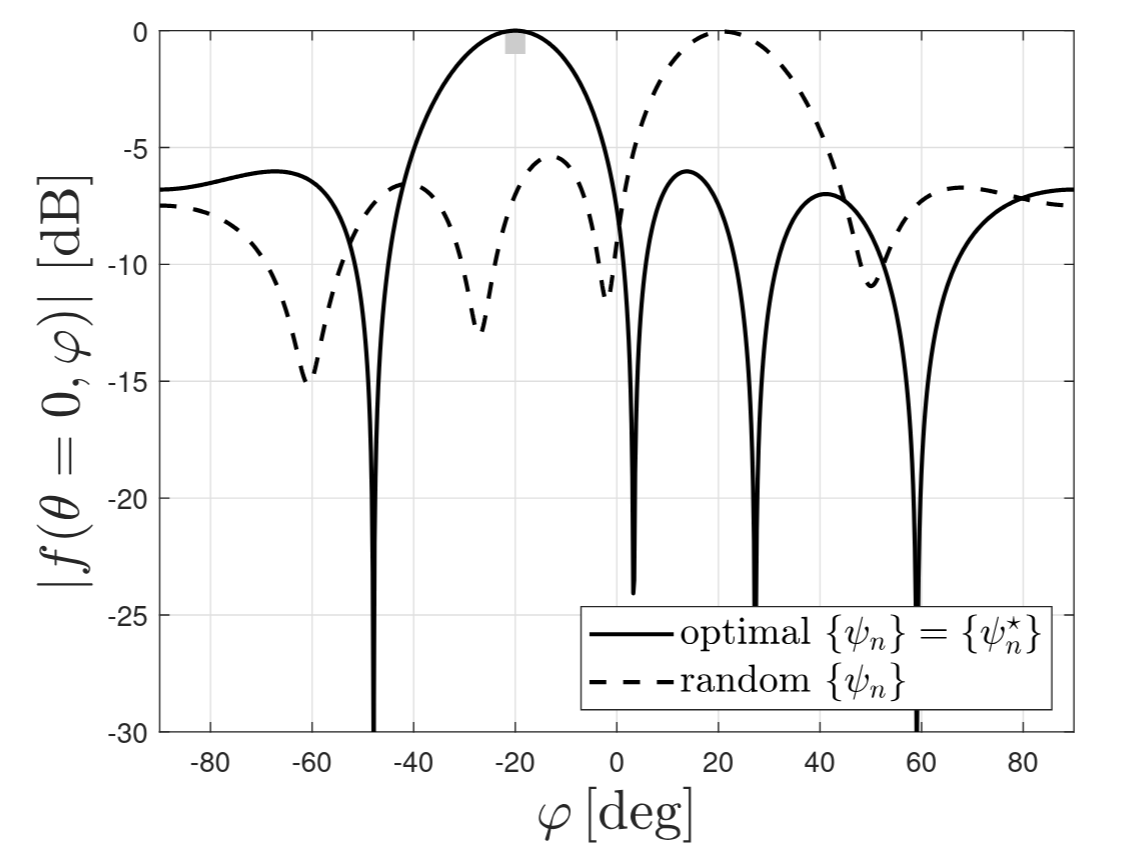
\includegraphics[width=0.8\textwidth]{chapter2/amplitude_array_response_of_ULA.png}
    }
    \vspace{0.8cm}
    \subfloat[Phase response $\angle f(\theta = 0, \varphi)$ \label{fig:phase_response}]{
        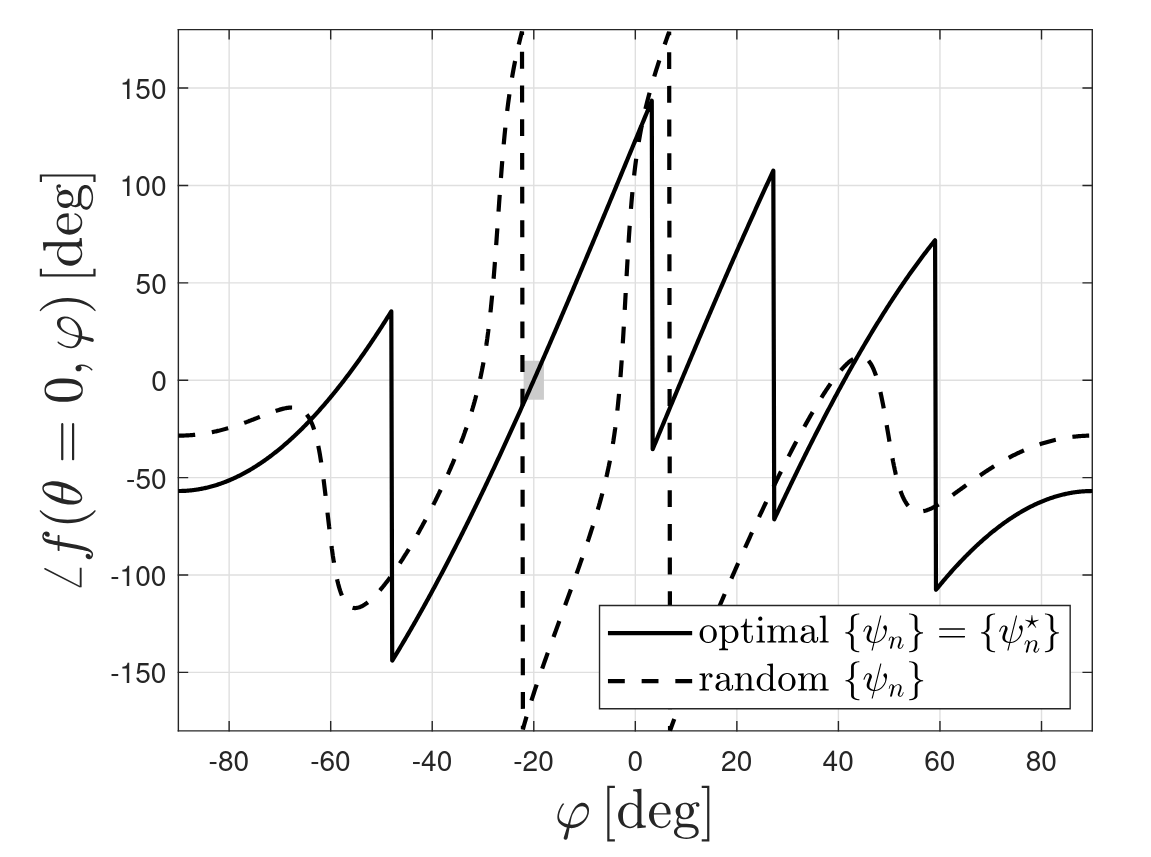
\includegraphics[width=0.8\textwidth]{chapter2/phase_array_response_of_ULA.png}
    }
    \caption{Example of the array response using $N = 5$, $d = \lambda/2$,
             for $\theta = 0$, with random $\boldsymbol{\psi}$}
    \label{fig:array_response_example}
\end{figure}

%**************************************************************


\subsection{Problem formulation}

Given the parameters introduced in \sectionname~\ref{sec:system_model}, we intend to identify an efficient
and scalable algorithm to identify acceptable realizations of $\boldsymbol{\psi}$, such that, in a
given support $[\theta^\star \pm \Delta\theta] \times [\varphi^\star \pm \Delta\varphi]$ (e.g., $\Delta\theta = \Delta\varphi = 1^\circ$):
\begin{enumerate}
    \item the amplitude $|f(\theta, \varphi)|$ satisfies the absolute floor
    $\log_{10} |f(\theta, \varphi)| \geq \varepsilon_a$
    (e.g., $\varepsilon_a = -0.7$, i.e.\ $|f| \geq 0.20$);
    \item the phase $\angle f(\theta, \varphi)$ is such that
    $|\angle f(\theta, \varphi) - \angle f(\theta^\star, \varphi^\star)| \leq \varepsilon_p$
    (e.g., $\varepsilon_p = 5^\circ$).
\end{enumerate}
To better visualize the problem, \figurename~\ref{fig:amplitude_response} and \figurename~\ref{fig:phase_response} also report the acceptable regions, obtained assuming $\Delta\varphi = 2^\circ$, $\varepsilon_a = -1\,\text{dB}$, and $\varepsilon_p = 10^\circ$, as shaded gray areas. Note that here, for simplicity, we only observe along a specific $\theta$ (namely, $\theta = 0^\circ$), which yields acceptable regions as rectangles. In general, when looking at the full support $[\theta^\star \pm \Delta\theta] \times [\varphi^\star \pm \Delta\varphi]$, acceptable regions become parallelepipeds.\\
To avoid extensive-search approaches, we can use\gls{RL} methods that draw a random realization $\boldsymbol{\psi}$, and then vary the values of the components $\psi_n$ to drive the array response to possibly fall within the acceptable regions (and hence declare $\boldsymbol{\psi}$ as a ``good'' antenna phase shift set).

\section{Reinforcement Learning}
\label{sec:reinforcement_learning}

\subsection{Reinforcement Learning and alternatives}
The problem of identifying valid beamforming configurations admits no closed-form solution in the general case, and the set of feasible phase-amplitude vectors forms a non-convex, high-dimensional region whose structure is not known a priori.
\begin{itemize}
    \item The configuration must be recovered at the symbol rate, ruling out per-instance optimization with budgets in the seconds/minutes range;
    \item The method must generalize across target directions $\varphi^\star$ without retraining or restarting;
    \item To support\gls{DDM}, repeated inferences at the same target direction must yield distinct valid configurations drawn from a sufficiently diverse distribution, so that the signal observed by an eavesdropper outside the protected angular region remains stochastic.
\end{itemize}
These requirements are most naturally framed as a demand for amortized optimization over a distribution of valid configurations: the cost of searching the feasible set is paid once, offline, in exchange for constant-time stochastic inference at deployment. The remaining design question is how to perform that amortization while preserving sample diversity.
\subsubsection{Derivative-free methods}
Derivative-free methods such as\gls{CMAES} or\gls{BO} solve the problem for a single target angle but offer no mechanism for transfer, and converge to point solutions rather than distributions. Each new $\varphi^\star$ requires a fresh search, with wall-clock costs incompatible with symbol-rate updates, and each search yields a single configuration. A natural amortization strategy is therefore \emph{supervised distillation}: run a derivative-free solver across a grid of target angles, collect the solutions, and train a regression model $\varphi^\star \mapsto (\boldsymbol{\psi}, \boldsymbol{\alpha})$. This approach was considered and rejected:
\begin{itemize}
    \item The feasible set is non-convex and multimodal in $\varphi^\star$: nearby target directions may admit valid configurations in disconnected regions of action space, and a regression model trained to interpolate between them will produce invalid outputs in the gaps;
    \item The supervised model inherits whatever biases the offline solver exhibits without any mechanism to discover better solutions than the labels it was given;
    \item A regression model is deterministic by construction: identical contexts produce identical actions, precluding the per-symbol diversity that dynamic modulation requires. Post-hoc injection of noise around a single learned point does not recover diversity over the feasible set, since perturbations of a valid configuration generally leave the feasible region given its disconnected structure.
\end{itemize}
Generative modeling of the feasible set (e.g. diffusion models) avoids the regression-interpolation problem by learning to sample from the distribution of valid configurations rather than predict a single output per angle and as such it is naturally aligned with the diversity requirement. This approach is viable in principle, but it requires a labeled dataset of valid configurations stratified by target direction, which inherits the same offline-solver bottleneck as supervised distillation. It also separates feasibility from performance: a generative model trained by maximum likelihood concentrates on the most common valid configurations, not the highest-performing or maximally diverse ones, and provides no optimization signal to shape the sampled distribution toward either security or beamforming quality.
\subsubsection{Gradient-based optimization}
Gradient-based optimization with a differentiable surrogate for the constraint check is a further alternative that, where the constraint structure admits a useful relaxation, can prove to be effective. In our setting, however, the validity condition must hold pointwise over a continuous angular support: both amplitude and phase must satisfy their respective bounds for all $(\theta, \varphi) \in [\theta^\star \pm \Delta\theta] \times [\varphi^\star \pm \Delta\varphi]$. A smooth surrogate evaluated at a finite sample of that region does not certify feasibility at unsampled points, and tightening the approximation by increasing sampling density leads to a non-smooth limit. Log-barrier formulations additionally require iterates to remain strictly feasible throughout optimization, an assumption that fails when configurations are initialized at random. These methods also produce point solutions rather than distributions, requiring a separate mechanism to recover the diversity needed for dynamic modulation. For these structural reasons, gradient-based relaxations are ill-suited to this constraint geometry.
\subsubsection{Contextual bandit}
The contextual bandit formulation directly targets amortized optimization over a distribution of valid configurations without requiring a labeled dataset. At each episode the agent observes a context $c = [\cos\varphi^\star, \sin\varphi^\star, \rho_c]$, where $\rho_c \in [0,1]$ is the curriculum constraint progress, outputs an action $\mathbf{a} = [\boldsymbol{\psi}, \boldsymbol{\alpha}] \in \mathbb{R}^{2N}$ via a stochastic policy $\pi_\theta(\mathbf{a} \mid c)$, and receives a scalar reward $r(\mathbf{a}, c)$ measuring constraint satisfaction and beamforming quality; The episode terminates after a single step \cite{lattimore2020bandit}. The reward does not need to be differentiable; the policy gradient is estimated from samples, and the stochasticity of $\pi_\theta$ serves a dual role: it drives exploration over the continuous action space during training, and at deployment it provides the per-symbol diversity required for dynamic modulation, with each forward pass sampling a fresh valid configuration from the learned conditional distribution.\\
\\
In this work,\gls{PPO} is adopted as the policy gradient algorithm using the contextual bandit formulation. Its clipped surrogate objective bounds the policy update at each gradient step, preventing destructive updates during the high-variance early phases of training when the policy has not yet identified any feasible region \cite{schulman2017ppo}.\gls{CL} is applied to stabilize convergence by ensuring the agent receives a positive reward signal before the full constraint set and training angles are enforced as expanded in \subsubsectionname~\ref{subsubsec:curriculum_learning}.

\subsection{Probability theory and stochastic processes}
\gls{RL} problems are inherently stochastic as both the system evolution and the rewards may be subject to randomness. A random variable $X$ is a mapping from an outcome space to the real numbers, and its behavior is characterized by a probability distribution.\\
A key concept is the expected value which represents the average outcome of a random variable: $\mathbb{E}[X]$.
It is also often necessary to consider conditional expectations, such as $\mathbb{E}[X \mid Y]$ which describes the expected value of $X$ given knowledge of another variable $Y$. We can now define random process as a collection of random variables indexed by time, $\{X_t\}_{t \geq 0}$ used to model systems that evolve under uncertainty. In this context, both the system state and the observed rewards can be modeled as stochastic processes \cite{ross2019probability}.

\subsection{Objective functions}
\gls{RL} can be formulated as an optimization problem over time. The performance of a decision-making strategy is quantified through a cumulative reward, defined as:
\begin{equation}
    G_t = \sum_{k=0}^{\infty} \gamma^k R_{t+k}
\end{equation}
where $R_t$ is the reward at time $t$ and $\gamma \in [0,1)$ is the discount factor which determines the relative importance of immediate and future rewards.\\
The objective is to maximize the expected return $\mathbb{E}[G_t]$. In the contextual bandit formulation used in this work, each episode consists of a single step and terminates immediately, so the sum collapses to $G_t = R_t$: the discount factor becomes irrelevant and the agent maximises expected immediate reward directly.

\subsection{Markov property}
To make sequential decision problems manageable it is often assumed that the system satisfies the \emph{Markov property}. A stochastic process $\{S_t\}$ is defined as Markovian if the conditional distribution of the next state depends only on the current state:
\begin{equation}
    P(S_{t+1} \mid S_t, S_{t-1}, \dots, S_0) = P(S_{t+1} \mid S_t)
\end{equation}
This assumption implies that the current state contains all the relevant information needed to predict the future evolution of the system, consequently, it is not necessary to retain the full history of past states.\gls{MDP} provides a formal framework for\gls{RL}.

\subsection{Policy Gradient Methods}
In problems involving continuous action spaces, it is convenient to represent the policy using a parametric function. Let $\pi_\theta(a \mid s)$ denote a policy parameterized by a vector $\theta \in \mathbb{R}^d$; The objective is to find the parameters $\theta$ that maximize the expected return:
\begin{equation}
    J(\theta) = \mathbb{E}_{\pi_\theta}[G_0]
\end{equation}
In constrast with value-based methods, policy gradient methods optimize the policy parameters directly enabling a natural treatment of stochastic policies and continuous action spaces.
\subsection{Proximal Policy Optimization}

\gls{PPO} is a policy gradient method for\gls{RL} introduced by Schulman et al. at OpenAI \cite{schulman2017ppo}. It was mainly designed to address the instability and sample inefficiency that characterize earlier policy gradient algorithms, while being simpler to implement than\gls{TRPO}. It operates by collecting batches of experience via interaction with the environment using the current policy, and then performing multiple epochs of mini-batch stochastic gradient ascent on the clipped surrogate objective:
\begin{equation}
    L^{\mathrm{CLIP}}(\theta) = \mathbb{E}_t\!\left[\min\!\left(r_t(\theta)\,\hat{A}_t,\;\mathrm{clip}\!\left(r_t(\theta),\,1-\varepsilon,\,1+\varepsilon\right)\hat{A}_t\right)\right]
\end{equation}
where $r_t(\theta) = \pi_\theta(a_t \mid s_t)\,/\,\pi_{\theta_{\mathrm{old}}}(a_t \mid s_t)$ is the probability ratio between the updated and the old policy, $\hat{A}_t$ is the estimated advantage, and $\varepsilon$ is the clip parameter (typically $0.1$--$0.2$). The $\min$ operator ensures that the objective cannot benefit from moving $r_t$ outside the interval $[1-\varepsilon, 1+\varepsilon]$, bounding the policy update at each gradient step and preventing destructive updates during the high-variance early phases of training.

\subsection{MLP Policy}

Since the reward, defined via the amplitude and phase constraints, is a deterministic function of the current phase vector, the current state contains all information necessary to compute the reward with no dependence on the history of previous actions: the environment is fully observable and Markovian. Recurrent policies are designed for\gls{POMDP} \cite{kaelbling1998pomdp} where the hidden state must be inferred from a sequence of observations. This condition does not hold here; consequently, we adopt a standard MLP policy. The actor network uses two fully connected layers of 256 units with ReLU activations, and the critic uses three layers of 256 units, which is sufficient to represent both components while avoiding the additional complexity and variance introduced by recurrent architectures.              % Theoretical basis
% !TEX encoding = UTF-8
% !TEX TS-program = pdflatex
% !TEX root = ../tesi.tex

%**************************************************************
\chapter{Experimental setup}
\label{cap:chapter3}
%**************************************************************

%**************************************************************

\section{Development environment}

To ensure reproducibility of our experiments, this section details the hardware architecture, core software dependencies, and the key modeling simplifications adopted throughout this work. Our primary simplification is the reduction of the search space to a single dimension, fixing the elevation angle at $\theta = 0^\circ$ and optimizing exclusively over the azimuth.

\subsection{Programming language}

Given the field and scope of the problem, the Python programming language has been chosen because of the wealth of\gls{AI} research carried out in the language and the consequently established ecosystem of scientific libraries developed.  It is also a more well-know language in the scientific literature for future peer review and improvements.

\subsection{Development tools}

The choice of tool used to handle the python development environment was uv, a Python package and project manager. With respect to the classic approach of using pip with virtual environment and a requirements.txt file, uv enables the developer to have more granular control on the dependencies' versions. 


\begin{longtable}{@{}|l|p{7cm}|l|@{}}
\caption{Programming language \& Environment tools }
\label{tab:programming-environment}\\
\hline
\textbf{Component} & \textbf{Details} & \textbf{Version} \\
\hline
\endfirsthead

\multicolumn{3}{c}%
{{\tablename\ \thetable{} -- \textit{Continued from previous page}}} \\
\hline
\textbf{Component} & \textbf{Details} & \textbf{Version} \\
\hline
\endhead

\hline
\multicolumn{3}{r}{\textit{Continued on next page}} \\
\endfoot

\hline
\endlastfoot

Python & Main programming language for AI & ~=3.14.3 \\
\hline
uv & Fast Python package and project manager & 0.8.15 \\
\hline
ruff & Fast Python linter and code formatter & 0.15.6 \\
\end{longtable}
\newpage

\begin{longtable}{@{}|l|p{7cm}|l|@{}}
\caption{Python Libraries Used in the Project}
\label{tab:python-libraries}\\
\hline
\textbf{Library Name} & \textbf{Description} & \textbf{Version} \\
\hline
\endfirsthead

\multicolumn{3}{c}%
{{\tablename\ \thetable{} -- \textit{Continued from previous page}}} \\
\hline
\textbf{Library Name} & \textbf{Description} & \textbf{Version} \\
\hline
\endhead

\hline
\multicolumn{3}{r}{\textit{Continued on next page}} \\
\endfoot

\hline
\endlastfoot

gymnasium & Reinforcement learning environments & 1.2.3 \\
\hline
matplotlib & Plotting and visualization library & 3.10.8 \\
\hline
numpy & Numerical computing and array operations & 2.4.3 \\
\hline
scipy & Scientific computing and numerical algorithms & 1.17.1 \\
\hline
stable-baselines3 & Reinforcement learning algorithms & 2.7.1 \\
\hline
torch & Deep learning framework & 2.11.0 \\
\hline
triton & GPU programming language and compiler & 3.6.0 \\
\end{longtable}



\begin{longtable}{@{}|l|p{7cm}|l|@{}}
\caption{Hardware Used in the Project}
\label{tab:hardware-used}\\
\hline
\textbf{Component} & \textbf{Details} \\
\hline
\endfirsthead

\multicolumn{3}{c}%
{{\tablename\ \thetable{} -- \textit{Continued from previous page}}} \\
\hline
\textbf{Component} & \textbf{Details} \\
\hline
\endhead

\hline
\multicolumn{3}{r}{\textit{Continued on next page}} \\
\endfoot

\hline
\endlastfoot

CPU & Intel(R) Xeon(R) Gold 5418Y, CPU family: 6, Model: 143, Architecture: x86\_64 \\
\hline
GPU & Nvidia RTX 4090 \\
\end{longtable}

\section{Environment}
{\color{blue}I: Here you are explaining the principle of RL. You are not really describing your environment}
In this reinforcement-learning model, the agent is connected to its environment, and at each step of interaction the agent receives as input, \textit{i}, some indication of the current state, \textit{s}, of the environment; the agent then chooses an action, \textit{a}, to generate as output. The value of the action is calculated through a reward function, \textit{R}, and the behavior of the agent, \textit{B}, choosing actions that tend to increase the long-term sum of values \cite{kaelbling1996rl}. It learns over time by systematic trial and error, guided by an algorithm. 



\subsection{Training angles and sampling strategy}
{\color{blue}I: This first sentence is not clear to me}
In our\gls{ULA}-based DDM context, there are difficulties related to angle-dependent constraints and also sin-space sampling biases. 

\subsubsection{The Spatial Frequency Domain of a ULA}

The array response of a\gls{ULA} with $N$ elements and inter-element spacing $d$ is governed by the projection of the incoming wave vector onto the array axis. For an array oriented along the $y$-axis, with element positions $\mathbf{u}_n = [0,\, nd,\, 0]^\top$ for $n = 0, \ldots, N-1$, and a source at elevation $\theta = 0\degree $ and azimuth $\varphi$, the wave vector component along the array axis reduces to:
\begin{equation}
    k_y(\varphi) = \frac{2\pi}{\lambda}\sin\varphi
\end{equation}
The array manifold vector, the per-element phase accumulated by a plane wave arriving from $\varphi$, is therefore:
\begin{equation}
    \mathbf{v}(\varphi) = \left[1,\; e^{j\pi\sin\varphi},\; e^{j2\pi\sin\varphi},\; \ldots,\; e^{j(N-1)\pi\sin\varphi}\right]^\top
\end{equation}
where we have assumed $d = \lambda/2$. Given a steering vector $\mathbf{a} = [a_0, \ldots, a_{N-1}]^\top = [\alpha_n e^{j\psi_n}]$, the normalised array response is:
\begin{equation}
    f(\varphi) = \frac{1}{N}\mathbf{a}^H \mathbf{v}(\varphi) = \frac{1}{N}\sum_{n=0}^{N-1} \alpha_n\, e^{j(\pi\sin\varphi \cdot n - \psi_n)}
\end{equation}
A critical observation follows directly from this expression: $\varphi$ appears exclusively through $\sin\varphi$. Defining the direction cosine $u \triangleq \sin\varphi \in [-1, 1]$, the array response becomes a Fourier-like polynomial in $e^{j\pi u}$:
\begin{equation}
    f(u) = \frac{1}{N}\sum_{n=0}^{N-1} \alpha_n\, e^{j(\pi u \cdot n - \psi_n)}
\end{equation}
The array has no means of distinguishing between two directions that share the same value of $u$. Equivalently, all physics of the beamforming problem (gain, phase flatness, constraint satisfaction) is determined entirely by the spatial frequency $u$, not by the azimuth angle $\varphi$ per se.
\subsubsection{Angle-Dependent Constraint Difficulty}
\label{subsec:angle_dependant_constraint}
The\gls{DDM} validity constraint requires that, for a given target direction $\varphi^*$, the array response $f(\varphi)$ satisfies two conditions simultaneously over the angular support $[\varphi^* - \delta\varphi,\, \varphi^* + \delta\varphi]$ (with $\delta\varphi = 5\degree$ in the system under study):
\begin{align}
    \log_{10}|f(\varphi)| &\geq \varepsilon_a & &\text{(amplitude floor)}  \label{eq:ddm_amplitude} \\
    |\angle f(\varphi) - \angle f(\varphi^*)| &\leq \varepsilon_p & &\text{(phase flatness)} \label{eq:ddm_phase}
\end{align}
where $\varepsilon_p = 10\degree$ is the phase tolerance. Note that $\varepsilon_a$ is the raw base-10 logarithm of the normalised amplitude. The phase flatness condition is the binding constraint for secrecy: it forces the phase of the received signal to remain approximately constant within the legitimate receiver's angular neighbourhood while allowing it to vary freely, and ideally rapidly, outside. Because the array response depends only on $u = \sin\varphi$, the angular support maps to an interval in $u$-space of width:
\begin{equation}
    \Delta u(\varphi^*) = |\sin(\varphi^* + \delta\varphi) - \sin(\varphi^* - \delta\varphi)| = 2\cos\varphi^*\sin(\delta\varphi)
\end{equation}
This width is maximised at broadside and collapses toward zero at endfire, meaning that the feasible set of valid steering vectors is smallest at broadside. \figurename~\ref{fig:sampling_constraint_bandwidth} plots $\Delta u(\varphi^*)$ for the system under study: the constraint window spans $\Delta u = 0.174$ at $\varphi^* = 0\degree$ and only $\Delta u = 0.087$ at $\varphi^* = 60\degree$: exactly half as wide.
The array response $f(u)$ is a degree polynomial $(N-1) = 4$ in $z = e^{j\pi u}$; As $u$ sweeps across the constraint window, $z$ traces an arc of the unit circle in the complex plane. By the argument principle, any zero of $f$ that lies near this arc induces a rapid phase swing across the corresponding range of $u$: for the phase to remain within $\pm\varepsilon_p$ throughout the window, all four polynomial zeros must be kept well away from the constraint arc. The arc subtends an angle of $\pi\Delta u(\varphi^*)$ radians:
\begin{align}
    \varphi^*=0\degree&:\quad \pi \times 0.174 \approx 0.55\;\text{rad}\;(\approx 31\degree\;\text{of arc}) \\
    \varphi^*=60\degree&:\quad \pi \times 0.087 \approx 0.27\;\text{rad}\;(\approx 16\degree\;\text{of arc}) \\
    \varphi^*=80\degree&:\quad \pi \times 0.030 \approx 0.09\;\text{rad}\;(\approx 5\degree\;\text{of arc})
\end{align}
At broadside, all four zeros must collectively avoid a $31\degree$ arc, a severe geometrical restriction that confines valid zero configurations to a small subset of the possible arrangements confining valid steering vectors to a small, concentrated region of the $2N$-dimensional parameter space. Near endfire, the constraint arc shrinks to just $5\degree$, and almost any zero placement satisfies it since the feasible set of valid steering vectors is large and geometrically diverse.\\
The direct consequence is that valid steering vectors at broadside are structurally similar to one another: every valid solution must displace its polynomial zeros from the same substantial arc since they are all constrained to a tight cluster in the high-dimensional parameter space, sharing the same structural property and differing only in the exact placement of zeros outside the arc and in the global phase offset. At endfire, valid solutions are spread across a wide region of parameter space and are structurally diverse.

\begin{figure}[htbp]
    \centering
    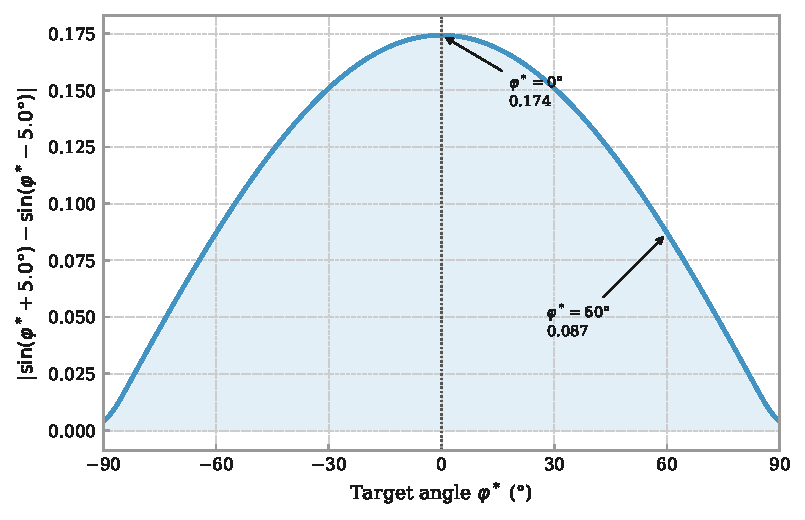
\includegraphics[width=0.75\textwidth]{images/chapter3/sampling_bandwidth.pdf}
    \caption{DDM constraint bandwidth in sin-space: broadside spans $0.174$ compared to $0.087$ at $60\degree$ resulting in a 2.0 ratio}
    \label{fig:sampling_constraint_bandwidth}
\end{figure}
\FloatBarrier

The matched-filter or\gls{DFT} steering vector, with phases $\psi_n = \pi\sin\varphi^* \cdot n$, is the canonical starting point for any beamformer: it maximises gain at $\varphi^*$ without imposing any further constraint. Under this choice, the array response phase increases linearly with $(\sin\varphi - \sin\varphi^*)$, giving a phase gradient at the target of:
\begin{equation}
    \frac{d\angle f}{d\varphi}\bigg|_{\varphi=\varphi^*} = \frac{N-1}{2}\,\pi\cos\varphi^*
\end{equation}
For $N = 5$ this evaluates to $2\pi\cos\varphi^*$ rad/rad, and the maximum phase deviation accumulated across the half-window $\delta\varphi$ is approximately:
\begin{equation}
    \Delta\angle f_{\max} \approx \frac{N-1}{2}\,\pi\cos\varphi^* \cdot \delta\varphi = 2\pi\cos\varphi^* \cdot \delta\varphi
\end{equation}
At broadside ($\varphi^* = 0\degree$, $\delta\varphi = 0.0873\,\text{rad}$) this gives $\Delta\angle f_{\max} \approx 31\degree$: more than three times the $\varepsilon_p = 10\degree$ tolerance. The crossover angle at which the\gls{DFT} solution just satisfies the phase constraint is:
\begin{equation}
    \varphi^*_{\text{cross}} = \arccos\!\left(\frac{\varepsilon_p}{\frac{N-1}{2}\pi\delta\varphi}\right) \approx 71\degree
\end{equation}
\figurename~\ref{fig:sampling_dft_deviation} confirms this threshold numerically: the\gls{DFT} deviation exceeds $\varepsilon_p$ for all $|\varphi^*| < 71\degree$, covering the entire range from $0\degree$ to $60\degree$. \figurename~\ref{fig:sampling_phase_curves} shows the detailed phase deviation curves for four representative target angles.
Since the\gls{DFT} solution maximises the inner product between the steering vector and the array manifold at $\varphi^*$, it is the attractor of any gradient ascent on received power, yet the valid broadside cluster sits elsewhere, separated from the\gls{DFT} solution by a broad infeasible region that provides no gradient bridge. The magnitude of this gap, a.k.a. how far the solution is from the valid cluster in steering vector space, grows as $\cos\varphi^*$ and is most severe at broadside.

\begin{figure}[htbp]
    \centering
    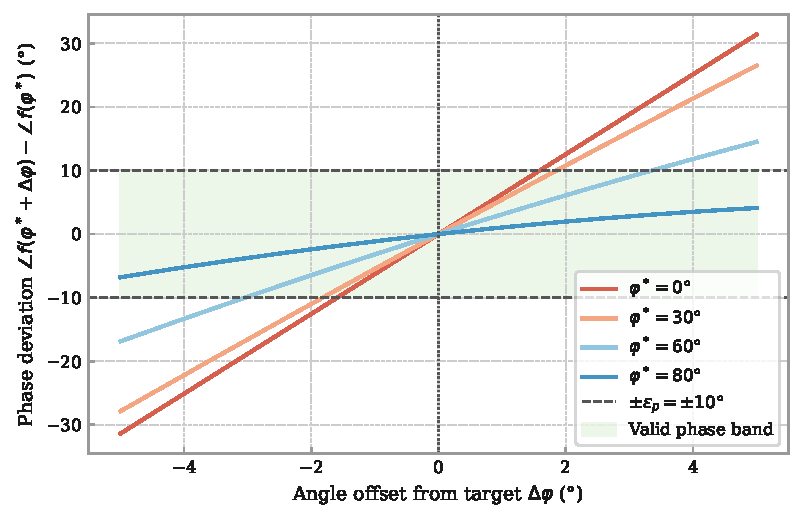
\includegraphics[width=0.75\textwidth]{images/chapter3/sampling_phase_curves.pdf}
    \caption{\gls{DFT} beamformer phase across $\pm5.0\degree$ window. Curves outside the green band require a non-\gls{DFT} solution.}
    \label{fig:sampling_phase_curves}
\end{figure}

\begin{figure}[htbp]
    \centering
    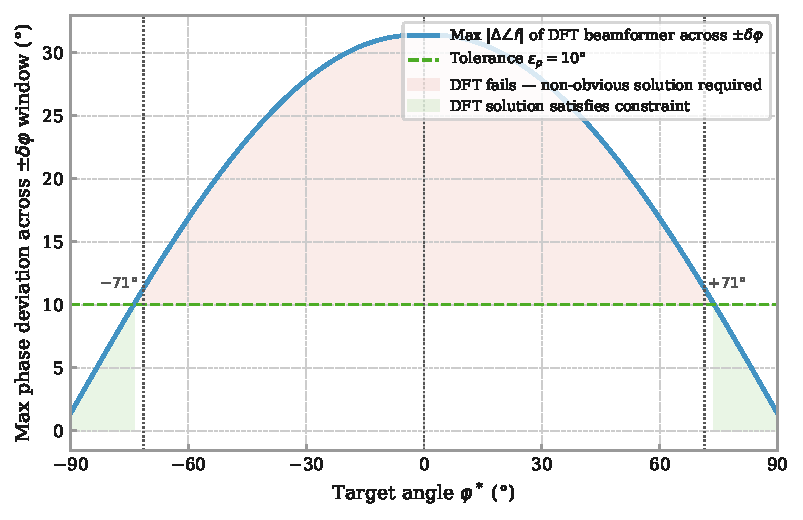
\includegraphics[width=0.75\textwidth]{images/chapter3/sampling_dft_deviation.pdf}
    \caption{\gls{DFT} beamformer phase deviation with N=5 elements. At broadside ($0\degree$): $31\degree$,\gls{DFT}-only solutions are valid only for $|\varphi^*| > 71\degree$}
    \label{fig:sampling_dft_deviation}
\end{figure}
\FloatBarrier

\subsubsection{The Sin-Space Sampling Bias}
\label{subsec:sin-space_sampling_bias}
The constraint difficulty described in \subsectionname~\ref{subsec:angle_dependant_constraint} is an intrinsic property of the\gls{ULA} geometry that can be exacerbated or alleviated by the chosen sampling strategy. 
Training angle sets are most naturally specified in degrees of azimuth: $\varphi \in \{-90\degree, -89\degree, \ldots, +90\degree\}$, a set of 181 angles uniformly spaced in $\varphi$. The Jacobian of the mapping $u = \sin\varphi$ is $du/d\varphi = \cos\varphi$, so equal angular steps $\Delta\varphi$ correspond to unequal $u$-space displacements:
\begin{equation}
    \Delta u \approx \cos\varphi^* \cdot \Delta\varphi
\end{equation}
Near broadside, ($\cos\varphi^* \approx 1$) each $1\degree$ step produces the largest possible displacement in $u$-space causing sampled angles to be spread across the broadside region while near endfire ($\cos\varphi^* \to 0$) the same angular step produces a negligible $u$-displacement causing large numbers of angles to crowd into a vanishingly narrow spatial-frequency band.
When $\varphi$ is drawn uniformly from $[-90\degree, 90\degree]$, the induced distribution of $u = \sin\varphi$ follows the arcsine law, $p(u) = 1/(\pi\sqrt{1-u^2})$, which diverges at $u = \pm 1$ and attains its minimum $1/\pi$ at $u = 0$. The histogram is therefore U-shaped: density is lowest at broadside and spikes sharply at the endfire limits, as shown by the blue histogram in \figurename~\ref{fig:sampling_density}. The red histogram shows the distribution obtained by sampling $u$ uniformly in $[-1, 1]$, flat by construction.
Concretely, with 181 uniform-in-$\varphi$ angles: the endfire neighbourhood $|\varphi| > 80\degree$ contributes 22 angles yet spans only ${\approx}3\%$ of the full $u$-domain. The broadside neighbourhood $|\varphi| < 10\degree$ contributes a comparable 21 angles but spans ${\approx}35\%$ of the $u$-domain, leaving it severely undersampled relative to its spatial-frequency extent.

\begin{figure}[htbp]
    \centering
    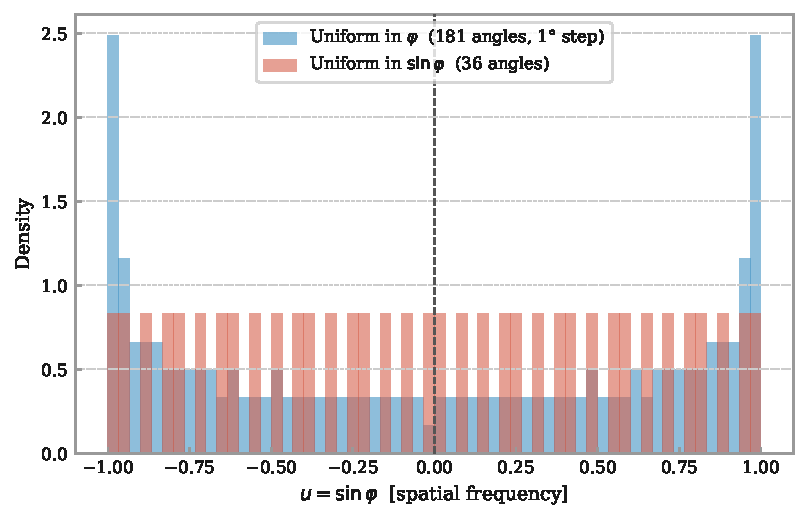
\includegraphics[width=0.75\textwidth]{images/chapter3/sampling_density.pdf}
    \caption{Angle density in sin-space. Sampling 181 angles with 1\degree step results in crowding in endfire while sin sampling results in a flat scheme.}
    \label{fig:sampling_density}
\end{figure}

\subsubsection{Compound Effect and Adopted Sampling Strategy}

The physical difficulty \subsectionname~\ref{subsec:angle_dependant_constraint} and the sampling bias \subsectionname~\ref{subsec:sin-space_sampling_bias} are independent mechanisms, but they can combine adversarially.
The physical difficulty means that each broadside episode is unlikely to yield a valid solution easily, so the policy needs many broadside episodes to accumulate enough successful exploration to converge on the valid cluster while the sampling bias simultaneously ensures that broadside receives the fewest episodes per unit of $u$-space: precisely the region that most needs a large exploration budget. Meanwhile, endfire receives the most episodes per $u$-space unit despite needing the least: the feasible set is large, the\gls{DFT} solution is already valid for $|\varphi^*| > 71\degree$, and the policy consolidates endfire performance quickly resulting in abundant valid rewards from endfire dominating the policy gradient leading to reinforcing strategies that work at endfire. These same strategies do not transfer to broadside as the valid solutions occupy a structurally different, concentrated cluster in steering vector space and because broadside episodes are infrequent, the corrective signal from broadside failures is too sparse to drive the policy toward the correct region.\\
Sampling training angles uniformly in $u = \sin\varphi$ and mapping back via $\varphi = \arcsin(u)$, produces the flat distribution shown in red in \figurename~\ref{fig:sampling_density}. This corrects the secondary cause: it equalises exploration budget across all spatial frequencies, shifting episodes away from the already mastered endfire region and toward the underexplored broadside region.
Addressing the physical difficulty, instead, requires an exploration regime capable of navigating a high-dimensional parameter space toward a geometrically concentrated feasible set and\gls{CL} provides a principled mechanism: the agent first builds intuition for what valid solutions look like at broadside angles, then transfers and refines that understanding as the constraint tightens and finally the target angles expand to the desired $[-90\degree, 90\degree]$.

\subsection{Training configuration}

\subsubsection{State Space}

The state space $\mathcal{S}$ encodes the target azimuth angle $\varphi$ together with the current constraint curriculum progress $\rho_c \in [0,1]$ (\subsubsectionname~\ref{subsubsec:curriculum_learning}). Rather than passing the raw angle in radians, the angular component is represented as its trigonometric projections:

\begin{equation}
    \mathbf{s} = \bigl[\cos(\varphi),\; \sin(\varphi),\; \rho_c\bigr] \in [-1, 1]^2 \times [0, 1]
\end{equation}
The trigonometric encoding keeps the angular components bounded in $[-1, 1]$ and preserves angular proximity in Euclidean distance. Including $\rho_c$ as a third observation component makes the environment \emph{stationary}: at any fixed pair $(\varphi,\,\rho_c)$ the optimal action and expected reward are fully determined, so the policy can condition its output on the current tightness of the physical constraints and avoid conflating loose early-curriculum episodes with tight late-curriculum episodes at the same target angle. The observation space is a bounded continuous box $\mathcal{S} \subseteq [-1,1]^2 \times [0,1]$, with all three components of type \texttt{float32}.

\subsubsection{Action Space}
The action space $\mathcal{A}$ is a continuous box of dimension $2N$ where $N$ is the number of antenna elements in the\gls{ULA}. Each action vector is split into two equal halves:

\begin{equation}
    \mathbf{a} = [\underbrace{a_1, \dots, a_N}_{\text{phase}},\;
    \underbrace{a_{N+1}, \dots, a_{2N}}_{\text{amplitude}}] \in [-1, 1]^{2N}
\end{equation}
All components are normalized to the interval $[-1, 1]$ as required by the\gls{PPO} policy network. At inference time, the two halves are rescaled into their physical ranges. The phase components are mapped to $[0, 2\pi]$:

\begin{equation}
    \varphi_n = a_n \cdot \pi + \pi, \quad n = 1, \dots, N
\end{equation}

and the amplitude components are mapped to $[0, 1]$:

\begin{equation}
    \alpha_n = a_{N+n} \cdot 0.5 + 0.5, \quad n = 1, \dots, N
\end{equation}
This symmetric normalization keeps the action distribution centered around zero, which is beneficial for the stability of gradient-based policy optimization.
\begin{figure}[htbp]
    \centering
    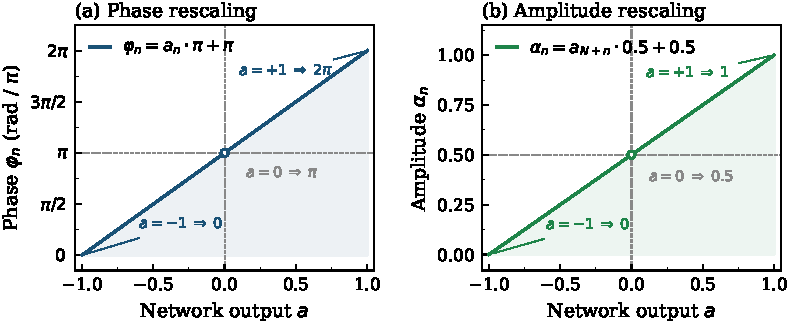
\includegraphics[width=0.75\textwidth]{images/chapter3/network_output_mapping.pdf}
    \caption{Phase and amplitude mapping}
    \label{fig:network_output_mapping}
\end{figure}
\FloatBarrier
An alternative physics-informed residual parameterisation, in which the action encodes corrections to the\gls{DFT} steering vector rather than absolute phases, is evaluated in \subsectionname~\ref{subsec:physics_informed} and visualized in \figurename~\ref{fig:physics_informed_network_output_mapping}.
\begin{figure}[htbp]
    \centering
    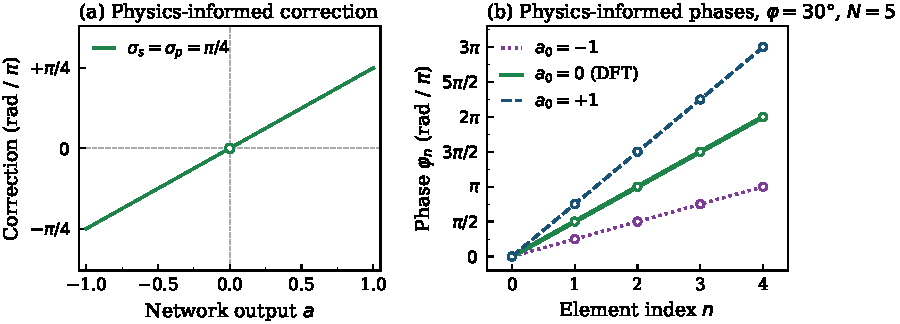
\includegraphics[width=0.75\textwidth]{images/chapter3/physics_informed_mapping.pdf}
    \caption{Phase physics informed mapping}
    \label{fig:physics_informed_network_output_mapping}
\end{figure}

\subsubsection{Transition Function}

The environment is formulated as a \textit{contextual bandit}, meaning that every episode consists of exactly one interaction step; At the beginning of each episode, a target angle $\varphi$ is sampled uniformly at random from the discrete set of training angles $\varphi_{\text{train}}$:

\begin{equation}
    \varphi \sim \mathcal{U}(\varphi_{\text{train}})
\end{equation}
The agent observes the encoding $\mathbf{s} = [\cos\varphi, \sin\varphi, \rho_c]$, produces a single action $\mathbf{a}$, receives a scalar reward $r$, and the episode terminates immediately with \texttt{terminated = True}. There is no temporal state transition; the next state is irrelevant, since the episode ends after each step.\\
This bandit formulation is a deliberate and central architectural choice: the optimal beamforming configuration for a given $\varphi$ is stateless since it does not depend on any history of prior actions, and there is no sequential decision process to unroll. Casting the problem as a bandit therefore removes a layer of complexity that would otherwise be artificial, eliminates the credit assignment problem across time steps, and allows the agent to receive an immediate and unambiguous reward signal for every configuration it proposes. \\
Generalization across angles is achieved by randomizing $\varphi$ at each reset, forcing the policy to learn a direct mapping from angle encoding to beamforming configuration rather than momorizing a fixed solution for a single direction.
\subsubsection{Reward Function}
The reward signal $r$ is a composite of four tiers designed to guide the agent progressively from geometrically valid beam shapes toward configurations that jointly maximise the\gls{BER} performance of the legitimate receiver and the decoding difficulty for potential eavesdroppers. The design directly optimises communication and\gls{PLS} metrics rather than relying on beam geometry alone to imply them.

\subsubsection{Amplitude coherence terms.}
Before the soft constraint evaluation, two amplitude terms provide a base gradient over the element weights $\boldsymbol{\alpha} = [\alpha_1, \ldots, \alpha_N]^\top$:
\begin{equation}
    r_{\text{amp}} = 20\,\overline{\alpha} + 7\,\overline{\log\max(\alpha_n,\,0.01)}
\end{equation}
where $\overline{\alpha} = \frac{1}{N}\sum_n \alpha_n$ is the mean amplitude and the log term is the per-element mean of $\log(\alpha_n)$ clamped at $10^{-2}$. The linear term pushes all elements toward full power, while the log penalty imposes a large gradient near zero and discourages any element from being completely silenced. The clamp at $10^{-2}$ bounds the penalty at $\approx -6.5$ per element so the gradient does not vanish for fully-off elements.

\subsubsection{Soft constraint terms.}
The second tier evaluates the soft\gls{DDM} validity of the produced steering vector. Four statistics are extracted from the soft validation function evaluated over a 2D grid of $N_v = 40$ points per axis (a $40 \times 40$ grid within the support $[\theta_{\mathrm{ref}} \pm \delta_\theta] \times [\varphi \pm \delta_\varphi]$): the mean amplitude score $s_a \in [0,1]$, the mean phase score $s_p \in [0,1]$, the minimum phase sigmoid $p_{\min} \in [0,1]$, and the mean absolute phase deviation $\bar{\delta\varphi}$. The soft constraint reward is:
\begin{equation}
    r_{\text{val}} = 3\,s_a + 4\,s_p + p_{\min} - 2\,\frac{\bar{\delta\varphi}}{\pi}
\end{equation}
The four terms are additive, so each provides an independent gradient signal throughout training; Positive terms reward progress toward the feasible region even before full validity is achieved, while the penalty on $\bar{\delta\varphi}$ discourages large average phase errors that keep the gradient alive when the policy is far from the validation constraints.

\subsubsection{Legitimate receiver BER.}
The third tier directly optimises the\gls{BER} experienced by the intended receiver. Given the normalized array gain $|f^*|$ at the target direction and the curriculum-adjusted reference\gls{SNR} $\mathrm{SNR}_0$ (\subsubsectionname~\ref{subsubsec:curriculum_learning}), the received $E_s/N_0$ is $|f^*|^2 \cdot 10^{\mathrm{SNR}_0/10}$ and the theoretical $M$-\gls{PSK}\gls{BER} (with $M = 8$ throughout this work) is:
\begin{equation}
    B_{\text{legit}} = \mathrm{BER}_{M\text{-PSK}}\!\left(|f^*|^2 \cdot 10^{\mathrm{SNR}_0/10}\right)
\end{equation}
A log-scale\gls{BER} score maps this to a normalised reward in $[0, 1]$:
\begin{equation}
    \mathrm{BER\_score} = \frac{\log_{10} B_{\text{legit}} - \log_{10} 0.5}{\log_{10} B_{\text{target}} - \log_{10} 0.5}
\end{equation}
where $B_{\text{target}} = 10^{-4}$. The score equals $1$ when $B_{\text{legit}} \leq B_{\text{target}}$ (performance target met) and $0$ when $B_{\text{legit}} = 0.5$ (random guessing), providing a dense gradient over the full range of array gain. The\gls{BER} reward is:
\begin{equation}
    r_{\text{ber}} = w_{\text{ber}} \cdot \mathrm{BER\_score}, \quad w_{\text{ber}} = 5
\end{equation}
This term is applied unconditionally, without gating on validity, since amplitude coherence that increases array gain simultaneously improves the soft constraint scores, making a gate unnecessary and harmful to gradient flow.

\subsubsection{Pre-validation secrecy incentive.}
The fourth pre-validation term rewards configurations that produce high\gls{BER} at eavesdropper positions. For each angle $\varphi_e$ in the training set satisfying $|\varphi_e - \varphi| > 10^\circ$, the eavesdropper\gls{BER} is computed accounting for both the received\gls{SNR} and the phase offset relative to the legitimate receiver:
\begin{equation}
    B_e(\varphi_e) = \mathrm{BER}_{M\text{-PSK}}\!\left(|f(\varphi_e)|^2 \cdot 10^{\mathrm{SNR}_0/10},\; \angle f(\varphi_e) - \angle f^*\right)
\end{equation}
The phase-aware\gls{BER} formula accounts for the fact that a phase error of $\pi/M$ places the received symbol on a decision boundary, maximising decoding errors regardless of\gls{SNR}. The unweighted mean eavesdropper\gls{BER} $\bar{B}_e$ (every eavesdropper angle counted equally, so that low-amplitude sidelobe angles receive the same gradient signal as main-beam directions) defines the secrecy\gls{BER} gap:
\begin{equation}
    \Delta B = \bar{B}_e - B_{\text{legit}} \in [-0.5,\; 0.5]
\end{equation}
A positive gap indicates that eavesdroppers on average experience a higher error rate than the legitimate receiver. The pre-validation secrecy reward is:
\begin{equation}
    r_{\text{sec}} = 5\,\max(0,\, \Delta B)
\end{equation}
Only positive gaps are rewarded before validity is confirmed, so early exploration is not penalised for failing to achieve secrecy before the beam shape itself is geometrically valid.

\subsubsection{Validity bonus and secrecy penalties.}
When the hard validity check passes, a structured validity bonus reinforces secrecy objectives:
\begin{equation}
    r_{\text{valid}} = w_\varphi \cdot 20 + 25\,\Delta B + w_{\text{wc}} \cdot \Delta B_{\min} - 35\,f_{\text{low}} + 15\,|f^*|
\end{equation}
where:
\begin{itemize}
    \item $w_\varphi = 1 + |\cos\varphi| \in [1, 2]$ is an angle-dependent weight that assigns double credit to broadside solutions, compensating for the structural difficulty at $\varphi \approx 0^\circ$ described in \subsectionname~\ref{subsec:angle_dependant_constraint}.
    \item $\Delta B_{\min} = B_{e,\min} - B_{\text{legit}}$ is the worst-case secrecy gap, where $B_{e,\min}$ is the minimum\gls{BER} across all eavesdropper angles (the easiest-to-decode adversary). The weight is $w_{\text{wc}} = 80$ if $\Delta B_{\min} < 0$ and $w_{\text{wc}} = 50$ otherwise, imposing a stronger penalty when the worst-case eavesdropper outperforms the legitimate receiver.
    \item $f_{\text{low}}$ is the fraction of eavesdropper angles with $B_e < 0.1$, penalising solutions that leave a large proportion of the angular space trivially decodable.
    \item The $15|f^*|$ term provides a gradient, pushing the array gain above the constraint floor toward maximum coherent gain; the\gls{BER} score saturates at $w_{\text{ber}}$ for any valid configuration at training\gls{SNR}, making this term the sole remaining gradient for increasing gain once validity is achieved.
\end{itemize}

\subsubsection{Total reward}
The total reward is:
\begin{equation}
    r = r_{\text{amp}} + r_{\text{val}} + r_{\text{ber}} + r_{\text{sec}} + \mathbf{1}[\text{valid}]\cdot r_{\text{valid}}
\end{equation}
with any non-finite value replaced by $r = -1$ to guard against numerical instability. The four pre-validation tiers provide dense gradient signals throughout training; the validity-gated tier provides the long-horizon objective that can only be earned by configurations that are simultaneously geometrically valid and secrecy-aware.


\subsubsection{Curriculum Learning}
\label{subsubsec:curriculum_learning}
Training a policy directly against the final, tightest physical constraints and the full angular range from the first iteration is inefficient as shown in \subsectionname\ref{subsec:curriculum_flattened}: the feasible region is small, the\gls{BER} and secrecy rewards are rarely triggered, and the reward landscape is nearly flat for most of the early training budget. A structured curriculum therefore progressively tightens the constraints and expands the range of training angles as training advances \cite{bengio2009curriculum}. Two independent progress scalars govern the curriculum:
\begin{equation}
    \rho_c = \min\!\left(\frac{t}{T \cdot r_c},\, 1\right), \qquad
    \rho = \min\!\left(\frac{t}{T \cdot r_s},\, 1\right)
\end{equation}
where $T$ is the total training budget, $r_c = 0.12$ is the constraint curriculum ratio (constraints reach their final values at $12\%$ of $T$), and $r_s = 0.20$ is the angle expansion ratio (the full angular range is unlocked at $20\%$ of $T$). The constraint progress $\rho_c$ is also included as the third observation component, making the environment stationary across curriculum stages.

\subsubsection{Amplitude tolerance $\epsilon_a$.}
The amplitude floor is annealed as:
\begin{equation}
    \epsilon_a(\rho_c) = -6 + 5.3\,\rho_c
\end{equation}
At $\rho_c = 0$ the floor sits at $-6$, imposing $|f| \geq 10^{-6} \approx 0$ that means effectively no amplitude constraint. By $\rho_c = 1$ it has risen to $-0.7$, requiring $|f| \geq 10^{-0.7} \approx 0.20$ everywhere in the window.

\subsubsection{Phase tolerance $\epsilon_p$.}
The maximum allowable phase deviation is tightened monotonically:
\begin{equation}
    \epsilon_p(\rho_c) = 30^\circ - 20^\circ \cdot \rho_c
\end{equation}
The agent begins with a generous $30^\circ$ phase margin, which accepts a wide range of steering vectors, and converges to a strict $10^\circ$ tolerance by the end of the constraint curriculum.

\subsubsection{Reference SNR.}
The reference transmit\gls{SNR} used for\gls{BER} reward evaluation is also annealed:
\begin{equation}
    \mathrm{SNR}_0(\rho_c) = 20\,\text{dB} - 3\,\text{dB} \cdot \rho_c
\end{equation}
Starting at $20\,\text{dB}$ provides a strong, unambiguous\gls{BER} gradient early in training. The\gls{SNR} decreases to $17\,\text{dB}$ by the end of the constraint curriculum, tightening the performance target as the beam quality requirement tightens simultaneously.

\subsubsection{Angle range curriculum.}
Before angle expansion begins (first $7\%$ of timesteps), the agent trains exclusively on broadside-adjacent angles $|\varphi| \leq 10^\circ$, where the\gls{DDM} feasibility problem is most constrained. The reachable training angle range then expands linearly from $\pm 10^\circ$ to $\pm 90^\circ$ between $7\%$ and $20\%$ of total timesteps:
\begin{equation}
    \varphi_{\max}(t) =
    \begin{cases}
        10^\circ & t < 0.07\,T \\[4pt]
        10^\circ + 80^\circ \cdot \dfrac{t/T - 0.07}{0.13} & 0.07\,T \leq t < 0.20\,T \\[4pt]
        90^\circ & t \geq 0.20\,T
    \end{cases}
\end{equation}
This staged expansion ensures the policy first builds valid broadside solutions before being exposed to the easier endfire angles, which would otherwise dominate the policy gradient.

\subsubsection{Broadside-biased sampling.}
During the expansion phase, sampling is biased toward the broadside region $|\varphi| \leq 30^\circ$ (region A) over the wider angular range (region B) through three equal-duration stages:
\begin{center}
\begin{tabular}{cccc}
\hline
Stage & Timestep range & $P(\text{region A})$ & $P(\text{region A})$ \\
\hline
1 & $[\phantom{0}7\%,\; 38\%]\,T$ & $80\%$ & $20\%$ \\
2 & $[38\%,\; 69\%]\,T$ & $60\%$ & $40\%$ \\
3 & $[69\%,\; 100\%]\,T$ & $50\%$ & $50\%$ \\
\hline
\end{tabular}
\end{center}
The three stages divide the period from expansion start to end of training into three equal thirds, each spanning $31\%$ of $T$. The reduction from $80\%$ to $50\%$ is deliberately slow: broadside solutions remain structurally harder than endfire solutions even after the angle range is fully open, so a sustained bias toward $|\varphi| \leq 30^\circ$ continues to provide corrective gradient throughout training. The final $50/50$ split preserves balance without starving any part of the angular range. \figurename~\ref{fig:curriculum_overview} summarises all four curriculum dimensions on a shared time axis, with the four training phases indicated by background shading.

\begin{figure}[htbp]
    \centering
    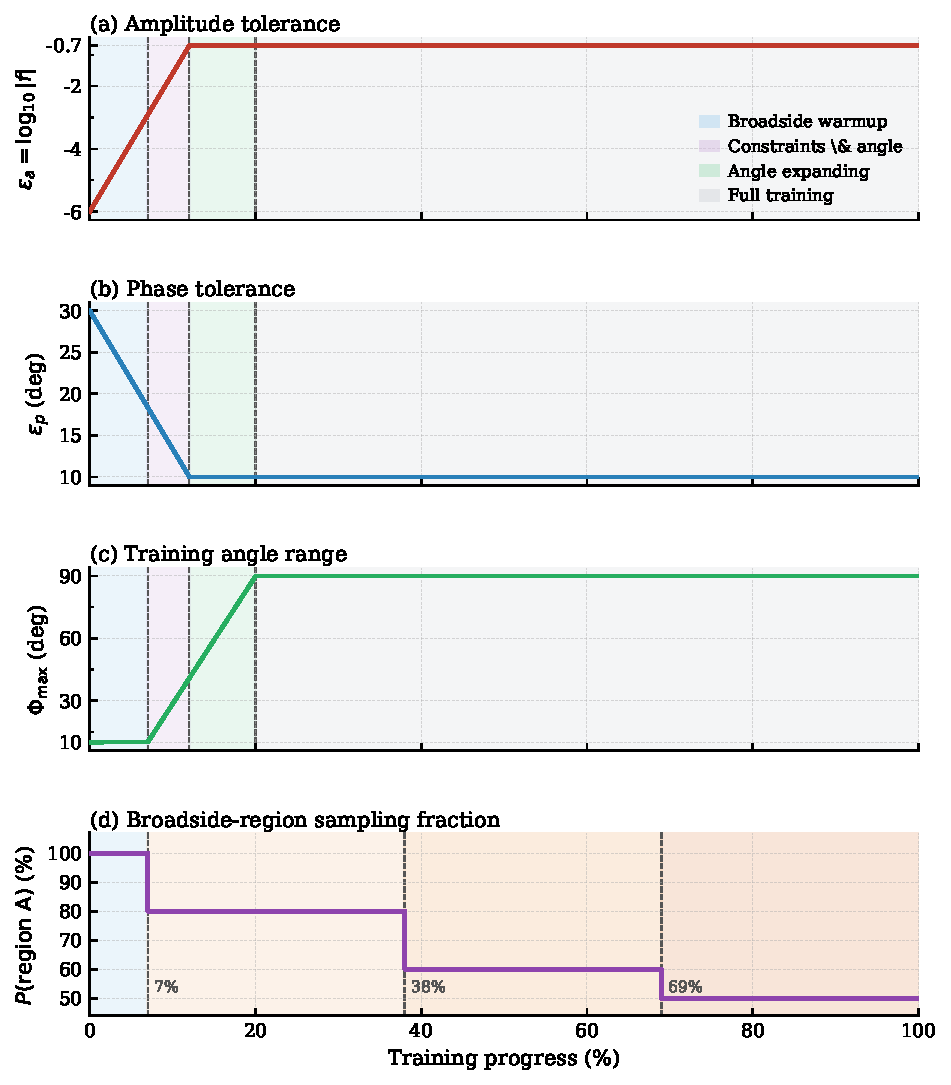
\includegraphics[width=0.85\textwidth]{images/chapter3/curriculum_overview.pdf}
    \caption{Complete curriculum schedule over training. Panel (a): amplitude floor $\varepsilon_a = \log_{10}|f|$ (raw base-10 logarithm of the normalised amplitude, not standard dB), rising from $-6$ ($|f| \geq 10^{-6} \approx 0$) to $-0.7$ ($|f| \geq 0.20$, or $-14\,\text{dB}$ standard). Panel (b): phase tolerance $\varepsilon_p$, from $30^\circ$ to $10^\circ$. Panels (a) and (b) complete at $12\%$ of total timesteps. Panel (c): training angle range, expanding from $\pm 10^\circ$ to $\pm 90^\circ$ between $7\%$ and $20\%$. Panel (d): broadside-region sampling fraction. Background shading marks the four phases: broadside warmup (blue, $0$--$7\%$), overlap (purple, $7$--$12\%$), angle-only expansion (green, $12$--$20\%$), and full training (grey, $20$--$100\%$). Dashed vertical lines mark transitions at $7\%$, $12\%$, and $20\%$; panel (d) uses orange shades for the three sampling stages ($7$--$38\%$, $38$--$69\%$, $69$--$100\%$).}
    \label{fig:curriculum_overview}
\end{figure}             % Tools utilized to train the model, parameters chosen
% !TEX encoding = UTF-8
% !TEX TS-program = pdflatex
% !TEX root = ../tesi.tex

%**************************************************************
\chapter{Validation}
\label{cap:chapter4}

\textcolor{magenta}{(I think it is a little bit unbalanced with respect to the other chapters. I would include it into the previous chapter. What do you think?}

The validation of the model behavior is a critical process to distinguish between plausible but incorrect results and valid ones.
In this work, validation is performed by comparing the simulated performance metrics with well-established theoretical results available in the literature. In particular, the\gls{BER} and\gls{SER} obtained through Monte Carlo simulations are evaluated against analytical expressions for M-\gls{PSK} modulation schemes over\gls{AWGN} channels, enabling the verification of both the quantitative accuracy of the results and the qualitative behavior of the system.
Through this validation framework, the model is assessed not only in terms of performance evaluation but also in terms of its consistency with established communication theory, providing confidence in the results presented in \chaptername~\ref{cap:chapter5}.
%**************************************************************

%**************************************************************
\section{Bit Error Rate}
\label{sec:ber}

\gls{BER} is one of the most widely used performance metrics for evaluating digital communication systems, defined as the ratio between the number of incorrectly received bits and the total number of transmitted bits.
\begin{equation}
    \label{eq:ber_definition}
    \text{BER} = \frac{N_{\text{errors}}}{N_{\text{total}}}
\end{equation}
\gls{BER} provides a measure of reliability of a communication link, capturing the cumulative impact of channel impairments such as noise, fading, interference, and hardware faults. In this work, it is evaluated as a function of the energy per bit to noise power spectral density ratio: $E_b/N_0$, to prefer a normalized metric that is independent of modulation order and bandwidth for fairer comparisons across different system configurations.

\section{Symbol Error Rate}

\gls{SER} is a performance metric defined as the probability that a transmitted symbol is incorrectly detected at the receiver. Unlike\gls{BER}, which operates at the bit level,\gls{SER} evaluates errors at the symbol level, making it useful for systems that employ multi-bit modulation schemes such as M-\gls{PSK}.

\begin{equation}
    \label{eq:ser_definition}
    \text{SER} = \frac{N_{\text{error symbols}}}{N_{\text{total symbols}}}
\end{equation}
As we have already specified,\gls{SER} is strongly dependent on the modulation order and the geometric arrangement of constellation points; as the constellation size increases, the symbols become more densely packed in the signal space, making them susceptible to noise and interference. Consequently, higher-order modulation schemes require higher energy-per-bit to maintain low\gls{SER}.

\section{Gray Coding}
The mapping between binary sequences and constellation symbols is crucial for determining the overall bit error performance. The most likely symbol errors occur between nearest neighbors in the signal constellation; a commonly adopted strategy to ensure that these neighbors differ by a single bit is Gray coding.
Under the assumption of gray-coded constellations and independent bit errors, the relationship between the\gls{SER} and the\gls{BER} can be approximated as:

\begin{equation}
    \label{eq:ber_ser_relation}
    \text{BER} \approx \frac{\text{SER}}{\log_2 M}
\end{equation}
This relationship becomes more accurate the higher the\gls{SNR} ratio is, where errors are dominated by nearest-neighbor symbol confusions.\\
In this work, gray mapping is utilized for all considered modulation schemes, ensuring consistent and fair comparison of\gls{BER} performance across different system configurations.
\begin{figure}[htbp]
    \centering
    \begin{subfigure}{0.45\textwidth}
        \includegraphics[width=\linewidth]{images/chapter4/2psk_gray_constellation.pdf}
        \caption{2-PSK gray coded constellation}
        \label{fig:2psk_gray_constellation}
    \end{subfigure}
    \hfill
    \begin{subfigure}{0.45\textwidth}
        \includegraphics[width=\linewidth]{images/chapter4/4psk_gray_constellation.pdf}
        \caption{4-PSK gray coded constellation}
        \label{fig:4psk_gray_constellation}
    \end{subfigure}
    \vspace{0.5cm}
    \begin{subfigure}{0.45\textwidth}
        \includegraphics[width=\linewidth]{images/chapter4/8psk_gray_constellation.pdf}
        \caption{8-PSK gray coded constellation}
        \label{fig:8psk_gray_constellation}
    \end{subfigure}
    \hfill
    \begin{subfigure}{0.45\textwidth}
        \includegraphics[width=\linewidth]{images/chapter4/16psk_gray_constellation.pdf}
        \caption{16-PSK gray coded constellation}
        \label{fig:16psk_gray_constellation}
    \end{subfigure}
    \caption{M-PSK (2, 4, 8, 16) gray coded constellations}
    \label{fig:mpsk_gray_constellation}
\end{figure}


\section{Theoretical M-PSK performance}
\label{sec:theoretical_mpsk}

For $M$-\gls{PSK} modulation over an\gls{AWGN} channel, the theoretical symbol error rate is:
\begin{equation}
    \label{eq:ser_mpsk}
    \mathrm{SER}(E_s/N_0) \approx 2\,Q\!\left(\sqrt{2\,\frac{E_s}{N_0}}\,\sin\frac{\pi}{M}\right), \quad M \geq 4
\end{equation}
where $Q(x) = \frac{1}{2}\,\mathrm{erfc}\!\left(x/\sqrt{2}\right)$ is the Q-function. For $M = 2$ (B\gls{PSK}), the expression is:
\begin{equation}
    \label{eq:ber_bpsk}
    \mathrm{BER}(E_b/N_0) = Q\!\left(\sqrt{2\,\frac{E_b}{N_0}}\right)
\end{equation}
Combining \equationname~\eqref{eq:ser_mpsk} with the Gray-coded\gls{BER} approximation of \equationname~\eqref{eq:ber_ser_relation} and substituting $E_s/N_0 = \log_2\!M \cdot E_b/N_0$ yields the theoretical\gls{BER} as a function of $E_b/N_0$ for $M \geq 4$:
\begin{equation}
    \label{eq:ber_mpsk}
    \mathrm{BER}(E_b/N_0) \approx \frac{2}{\log_2 M}\,Q\!\left(\sqrt{2\,\log_2\!M\cdot\frac{E_b}{N_0}}\,\sin\frac{\pi}{M}\right)
\end{equation}
These expressions serve as the analytical reference against which the Monte Carlo simulation results are compared in \chaptername~\ref{cap:chapter5}.

\section{M-PSK performance under a static phase offset}
\label{sec:ber_phase_offset}

The eavesdropper-directed reward terms of \chaptername~\ref{cap:chapter3} require the\gls{BER} experienced by a receiver whose decision regions are rotated by a static phase offset $\theta_e$ relative to the legitimate receiver, since the array response generally has a different phase at an eavesdropper direction $\varphi_e$ than at the target direction $\varphi^\star$. This section extends \equationname~\eqref{eq:ser_mpsk}--\eqref{eq:ber_mpsk} of \sectionname~\ref{sec:theoretical_mpsk} to this case.

Because the $M$-\gls{PSK} constellation is invariant under rotations of $2\pi/M$, and the decision regions are symmetric about each constellation point, any phase offset $\theta_e$ can be folded into an equivalent offset
\begin{equation}
    \delta = \min\!\left(\theta_e \bmod \frac{2\pi}{M},\;\; \frac{2\pi}{M} - \left(\theta_e \bmod \frac{2\pi}{M}\right)\right) \in \left[0,\, \frac{\pi}{M}\right]
    \label{eq:phase_offset_fold}
\end{equation}
measuring the distance of the rotated symbol from its nearest decision boundary (located at $\pm\pi/M$ from the symbol's nominal phase).

For $M = 2$, the classical result for a phase synchronization error applies directly: the signal's projection onto the decision axis is scaled by $\cos\delta$, giving
\begin{equation}
    \mathrm{BER}(E_b/N_0, \theta_e) = Q\!\left(\sqrt{2\,\frac{E_b}{N_0}}\,\cos\delta\right).
    \label{eq:ber_bpsk_phase_offset}
\end{equation}

For $M \geq 4$, the offset symbol sits closer to one of its two neighbouring boundaries than the other, so the two-sided nearest-neighbour approximation of \equationname~\eqref{eq:ser_mpsk} splits into two distinct terms, one per boundary:
\begin{align}
    \mathrm{SER}(E_s/N_0, \theta_e) \approx{} & Q\!\left(\sqrt{2\,\frac{E_s}{N_0}}\,\sin\!\Big(\max\big(\tfrac{\pi}{M} - \delta,\, 0\big)\Big)\right) \notag \\
    & {}+ Q\!\left(\sqrt{2\,\frac{E_s}{N_0}}\,\sin\!\left(\frac{\pi}{M} + \delta\right)\right)
    \label{eq:ser_mpsk_phase_offset}
\end{align}
where clamping the first argument at $0$ once $\delta \geq \pi/M$ (i.e.\ once the offset symbol has crossed the near boundary) saturates that term at its maximal value $Q(0) = 0.5$ rather than leaving it undefined. Combining \equationname~\eqref{eq:ser_mpsk_phase_offset} with the Gray-coded approximation of \equationname~\eqref{eq:ber_ser_relation} gives the\gls{BER} used for the eavesdropper reward terms of \chaptername~\ref{cap:chapter3}:
\begin{align}
    \mathrm{BER}(E_b/N_0, \theta_e) \approx{} & \frac{1}{\log_2 M}\Bigg[Q\!\left(\sqrt{2\log_2\!M\cdot\frac{E_b}{N_0}}\,\sin\!\Big(\max\big(\tfrac{\pi}{M}-\delta,\,0\big)\Big)\right) \notag \\
    & {}+ Q\!\left(\sqrt{2\log_2\!M\cdot\frac{E_b}{N_0}}\,\sin\!\left(\frac{\pi}{M}+\delta\right)\right)\Bigg]
    \label{eq:ber_mpsk_phase_offset}
\end{align}
clipped to $[0, 0.5]$ to remain a valid probability. As a sanity check, setting $\theta_e = 0$ (hence $\delta = 0$) collapses \equationname~\eqref{eq:ser_mpsk_phase_offset} to $2\,Q\!\left(\sqrt{2E_s/N_0}\sin(\pi/M)\right)$, recovering exactly \equationname~\eqref{eq:ser_mpsk}.

\section{Monte Carlo simulation}

The performance of the system is evaluated through Monte Carlo simulations, providing a flexible and widely adopted framework for estimating error rates. In this approach, the\gls{BER} and\gls{SER} are empirically estimated as:
\begin{equation}
    \widehat{\text{BER}} = \frac{N_{\text{bit errors}}}{N_{\text{total bits}}}, \quad
    \widehat{\text{SER}} = \frac{N_{\text{symbol errors}}}{N_{\text{total symbols}}}
\end{equation}
To characterize system performance,\gls{BER} and\gls{SER} are evaluated as functions of the energy-per-bit to noise power spectral density ratio, $E_b/N_0$, by varying the noise variance while keeping the transmitted signal energy constant. Given the stochastic nature of the simulation, the accuracy of the estimated error rates depends on the number of transmitted bits or until a predefined number of errors is observed, ensuring statistical reliability of the results.             % Explain and compare methods to validate model
% !TEX encoding = UTF-8
% !TEX TS-program = pdflatex
% !TEX root = ../tesi.tex

%**************************************************************
\chapter{Model results}
\label{cap:chapter5}
%**************************************************************

\section{Training results}

\subsection{Policy Parameters}
\figurename~\ref{fig:policy_parameters} illustrates the evolution of the key policy parameters throughout training: the action standard deviation and the learning rate.

\subsubsection{Standard Deviation}
The action standard deviation governs the stochasticity of the policy by controlling the spread of the Gaussian distribution from which actions are sampled during rollouts. As noted by Schulman et al.~\cite{schulman2017ppo}, maintaining sufficient exploration early in training is critical to avoid premature convergence to suboptimal policies. As visible in \figurename~\ref{fig:policy_parameters}, it decreases over the course of training, stabilising around $0.5$ toward the end. It can also be observed that the standard deviation does not collapse to near-zero values suggesting that it retained a healthy degree of residual stochasticity, avoiding the entropy collapse that can be indicative of over-exploitation~\cite{ahmed2019entropy}.\\
For any target angle, there exist many valid beamforming configurations made of phases and amplitudes that satisfy the amplitude and phase constraints forming a continuous solution manifold in the 2N-dimensional action space. Since\gls{PPO} parameterizes a unimodal Gaussian policy it cannot represent this multimodal structure directly, opting instead to converge to a wide distribution centered on the manifold. The action standard deviation value is therefore the natural consequence of maintaining sample diversity across the solution manifold with a unimodal policy class and not a sign of incomplete convergence. This conclusion is further reinforced in \sectionname~\ref{sec:diversity_analysis}.

\subsubsection{Clip range}

The clip range $\varepsilon$ is the central stability mechanism of\gls{PPO}, bounding the probability ratio between the new and old policy during each gradient update:

\begin{equation}
    L^{\mathrm{CLIP}}(\theta) = \mathbb{E}_t \left[ \min \left( r_t(\theta)\hat{A}_t,\ \mathrm{clip}(r_t(\theta),\, 1 - \varepsilon,\, 1 + \varepsilon)\hat{A}_t \right) \right]
\end{equation}
where $r_t(\theta) = \pi_\theta(a_t | s_t)/ \pi_{\theta_\mathrm{old}}(a_t | s_t)$. The clip range remained fixed at the default value of $\varepsilon = 0.2$ throughout training, as recommended by Schulman et al.~\cite{schulman2017ppo}. Its stability confirms that no adaptive clipping schedule was applied, and that the constraint was enforced uniformly across all gradient updates. 

\subsubsection{Learning rate}
The learning rate controls the step size of the Adam optimiser when updating the network weights. Training begins at $\alpha_{max} = 3 \times 10^{-4}$ and decays by a factor of $\delta = 0.998$ at the end of every rollout, down to a minimum of $\alpha_{min} = 1 \times 10^{-4}$. This slow decay lowers the effective step size as the policy matures, reducing the risk of overshooting near convergence. Once the curriculum reaches full constraint enforcement, the schedule addictionally monitors two instability signals over a sliding window of $W = 30$ rollouts:
\begin{enumerate}
    \item \textbf{reward drop detector:} if the most recent rollout mean reward falls more than $5\%$ below the window peak, a ramp is triggered;
    \item \textbf{validity crash detector:} if the fraction of rollouts that satisfy the constraints collapses to less than half of the window peak, a ramp is triggered.
\end{enumerate}
When either condition fires, the learning rate is linearly increased back to $\alpha_{\max}$ over $20$ rollouts, after which normal decay resumes with a cooldown of $50$ rollouts to prevent successive triggers from interfering with each other.

\begin{figure}[htbp]
    \centering
    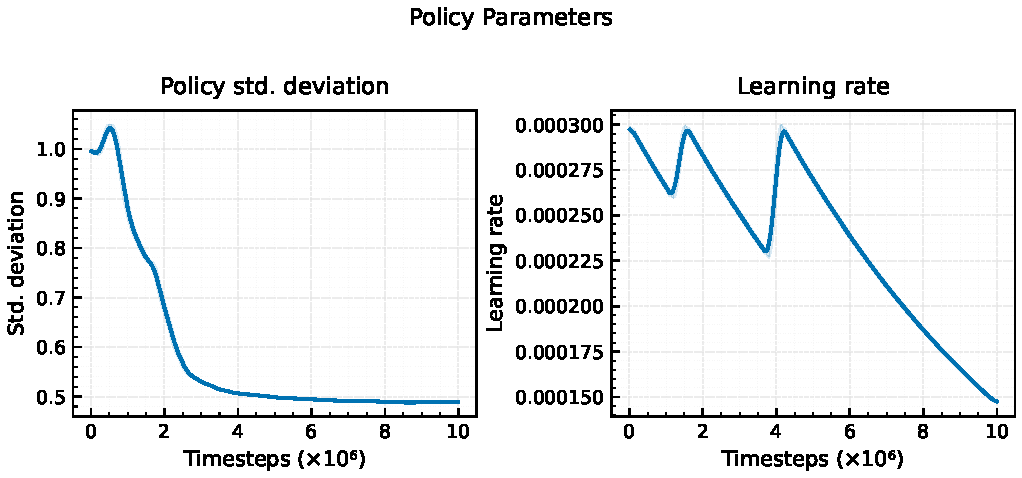
\includegraphics[width=1\textwidth]{images/chapter5/policy_parameters.pdf}
    \caption{The key policy parameters throughout training: the action standard deviation and the learning rate.}
    \label{fig:policy_parameters}
\end{figure}
\FloatBarrier

\subsection{PPO metrics}

\figurename~\ref{fig:ppo_diagnostic} reports three diagnostic metrics that characterise the quality of the policy updates and the critic's learning progress throughout training: the approximate KL divergence, the clip fraction, and the explained variance.

\subsubsection{Approximate KL divergence}
The approximate KL divergence measures how much the new policy has shifted from the old one following each gradient update, and serves as a key indicator of update stability. It is estimated as:

\begin{equation}
    \widehat{D}_{\mathrm{KL}} \approx \mathbb{E}_t \left[ \log \frac{\pi_{\theta_\mathrm{old}}(a_t | s_t)}{\pi_\theta(a_t | s_t)} \right]
\end{equation}
The approximate KL divergence begins at approximately $0.03$ at the start of training, decreases steadily, and increases to $0.03$ at the end of the run. The rapid decay and subsequent stability confirm that the clip range constraint ($\varepsilon = 0.2$) was effective in preventing excessively large policy updates. 

\subsubsection{Clip Fraction}
The clip fraction reports the proportion of samples in each rollout batch for which the probability ratio $r_t(\theta) = \pi_\theta(a_t | s_t) / \pi_{\theta_\mathrm{old}}(a_t|s_t)$ exceeded the clip boundary, i.e. fell outside the interval $[1 - \varepsilon,\,1]$. The clip fraction starts at approximately $0.2$ in the early stages of training and then increases, stabilising around $0.30$ for the rest of the run; The elevated values at the end suggests that the policy was undergoing substantial changes in the first updates, consistent with the high approximate KL divergence observed at the same time. As training progresses, the clip fraction settles into a healthy range, indicating that only a moderate proportion of samples were actively constrained by the clipping mechanism. 

\subsubsection{Explained Variance}
The explained variance quantifies how accurately the value function $V_\theta(s)$ predicts the empirical returns collected during rollouts:

\begin{equation}
    \mathrm{EV} = 1 - \frac{\mathrm{Var}(y - \hat{y})}{\mathrm{Var}(y)}
\end{equation}
where $y$ denotes the observed returns and $\hat{y}$ the value function predictions. A value of $1$ corresponds to perfect prediction, while values near $0$ or below indicate that the critic is no better than a constant baseline; The explained variance increases progressively towards $0.9$ over the course of training, demonstrating that the critic successfully learned to approximate the value landscape of the task.

\begin{figure}[htbp]
    \centering
    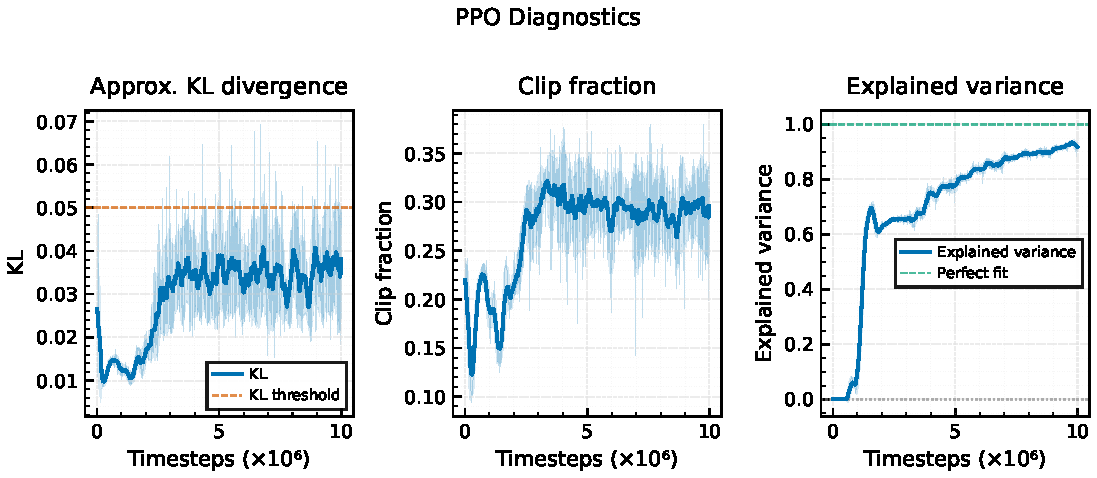
\includegraphics[width=1\textwidth]{images/chapter5/ppo_diagnostics.pdf}
    \caption{The three diagnostic metrics that characterise the quality of the policy updates and the critic's learning progress throughout training: the approximate KL divergence, the clip fraction, and the explained variance.}
    \label{fig:ppo_diagnostic}
\end{figure}
\FloatBarrier

\subsection{Training Convergence}

\figurename~\ref{fig:training_convergence} presents the two primary convergence indicators over the course of training: the mean episode reward and the valid-action rate. The reward curve (left axis) reflects how well the agent is optimising the beamforming objective, while the valid rate (right axis) measures the fraction of timesteps in which the agent produced a configuration that satisfied all amplitude and phase constraints. 

\begin{figure}[htbp]
    \centering
    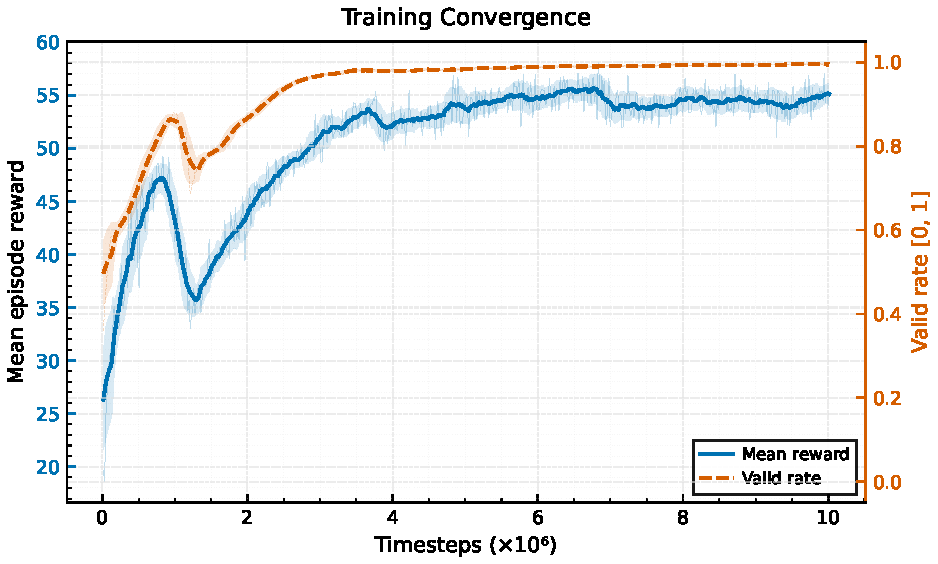
\includegraphics[width=0.80\textwidth]{images/chapter5/training_convergence.pdf}
    \caption{Training convergence: mean episode reward (left axis) and valid-action rate (right axis) over training timesteps.}
    \label{fig:training_convergence}
\end{figure}
\FloatBarrier

\subsection{Training losses}

\figurename~\ref{fig:training_losses} reports the four loss components optimised jointly by\gls{PPO} throughout training: the policy gradient loss, the value loss, the entropy loss, and the total combined loss. Monitoring these components is essential to distinguish between healthy optimisation dynamics and pathological behavior that may not be apparent from reward curves alone.

\subsubsection{Policy Gradient Loss}
The core actor loss measures how well the policy is being pushed toward higher-advantage actions. Under the clipped\gls{PPO} objective it is defined as:
\begin{equation}
    L^{\mathrm{PG}} = -\mathbb{E}_t \left[ \min \left( r_t(\theta)\hat{A}_t,\ \mathrm{clip}(r_t(\theta),\, 1 - \varepsilon,\, 1 + \varepsilon)\hat{A}_t \right) \right]
\end{equation}
where the negative sign arises because gradient descent is used to maximise expected reward. The clipping embedded in this objective is what distinguishes\gls{PPO} from vanilla policy gradient methods, and directly reflects whether policy updates are aligned with the advantage estimates~\cite{schulman2017ppo}. During healthy training this loss should remain small because large values indicate that updates are too aggressive.

\subsection{Value Loss}
The critic loss measures how accurately the value function predicts empirical returns, formulated as mean squared error between predicted state values and target returns:
\begin{equation}
    L^{\mathrm{VF}} = \mathbb{E}_t \left[ \left( V_\theta(s_t) - V_t^{\mathrm{target}} \right)^2 \right]
\end{equation}
This term is scaled by a coefficient $c_1$ before being added to the total loss, since an unscaled value loss would otherwise dominate the gradient signal. A higher value loss early in training is acceptable as long as it decreases as the critic learns since persistent high values would keep advantage estimates noisy and destabilise the actor.

\subsection{Entropy Loss}
The entropy loss measures the randomness of the policy's action distribution:

\begin{equation}
    L^{\mathrm{ENT}} = -\mathbb{E}_t \left[ H\!\left(\pi_\theta(\cdot \mid s_t)\right) \right] = \mathbb{E}_t \left[ \sum_a \pi_\theta(a \mid s_t) \log \pi_\theta(a \mid s_t) \right]
\end{equation}
A high-entropy policy is more exploratory, while a low-entropy policy is more deterministic. The entropy loss should gradually decrease over training as the policy becomes more confident.

\subsection{Total Loss}

All three components are combined into a single scalar objective minimized by the Adam optimizer at each gradient step:
\begin{equation}
    L^{\mathrm{TOTAL}} = L^{\mathrm{PG}} + c_1 \cdot L^{\mathrm{VF}} - c_2 \cdot L^{\mathrm{ENT}}
\end{equation}

As visualized in \figurename~\ref{fig:training_losses}, our losses behave in an ideal manner with values near $0$ at the end of the training.

\begin{figure}[htbp]
    \centering
    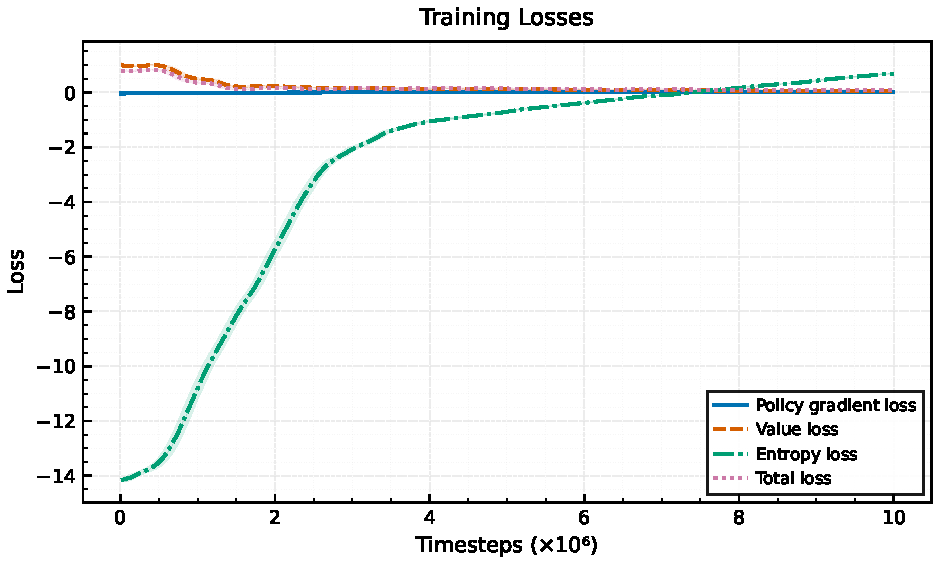
\includegraphics[width=0.85\textwidth]{images/chapter5/training_losses.pdf}
    \caption{The four loss components optimised jointly by\gls{PPO} throughout training: the policy gradient loss, the value loss, the entropy loss, and the total combined loss.}
    \label{fig:training_losses}
\end{figure}
\FloatBarrier

\subsection{Secrecy Performance}

\figurename~\ref{fig:secrecy_performance} tracks the\gls{BER} metrics throughout training on a logarithmic scale: the legitimate user\gls{BER}, the secrecy\gls{BER} and the minimum\gls{BER} of all possible eavesdropper angles. These curves reflect how well the agent is learning the physical-layer security objective: driving the legitimate\gls{BER} below the target threshold while maintaining a high eavesdropper\gls{BER}. 

\begin{figure}[htbp]
    \centering
    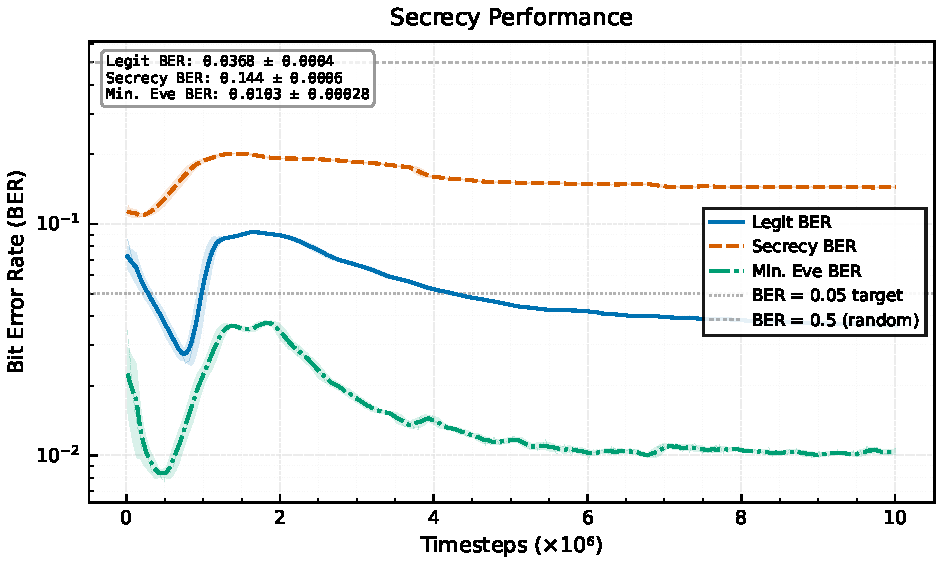
\includegraphics[width=0.75\textwidth]{images/chapter5/secrecy_performance.pdf}
    \caption{BER metrics throughout training: legitimate user\gls{BER}, secrecy\gls{BER}, and the minimum\gls{BER} of all possible eavesdropper angles on a logarithmic scale. Dashed reference lines at $\mathrm{BER}=0.05$ and $\mathrm{BER}=0.5$ are included for orientation.}
    \label{fig:secrecy_performance}
\end{figure}
\FloatBarrier
\subsection{Constraint Satisfaction}

\figurename~\ref{fig:constraint_satisfaction} shows the evolution of two constraint-related metrics during training: the valid-action rate and the fraction of eavesdropper directions with\gls{BER} below $0.1$. The valid rate measures how reliably the agent produces configurations that satisfy the amplitude floor and phase flatness constraints, while the low-BER fraction indicates how well the secrecy objective is met across the eavesdropper space.

\begin{figure}[htbp]
    \centering
    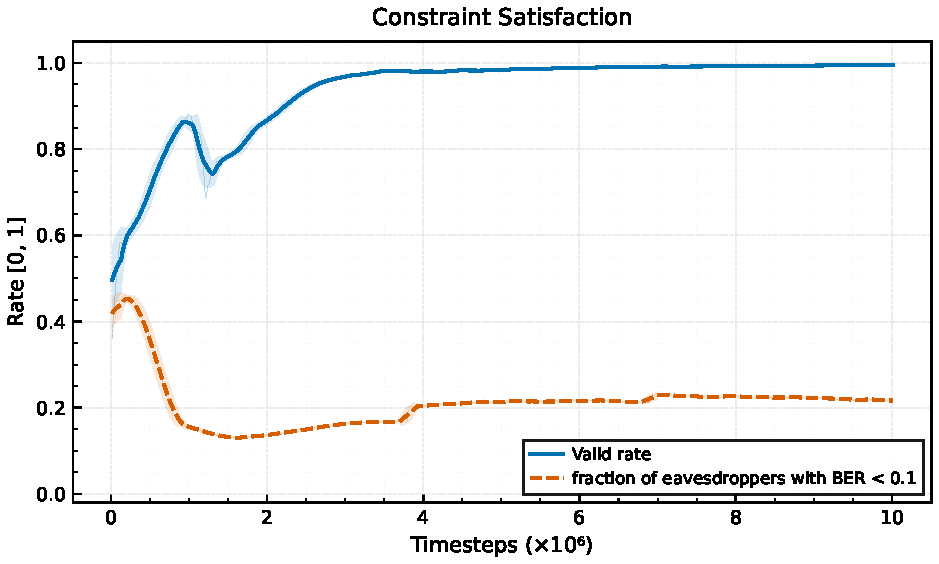
\includegraphics[width=0.80\textwidth]{images/chapter5/constraint_satisfaction.pdf}
    \caption{Constraint satisfaction throughout training: valid-action rate and fraction of eavesdropper directions with $\mathrm{BER} < 0.1$.}
    \label{fig:constraint_satisfaction}
\end{figure}
\FloatBarrier

\subsection{Training Overview}

\figurename~\ref{fig:training_overview} provides a concise four-panel summary of key training metrics: mean episode reward, valid-action rate, legitimate user\gls{BER}. and secrecy\gls{BER}.

\begin{figure}[htbp]
    \centering
    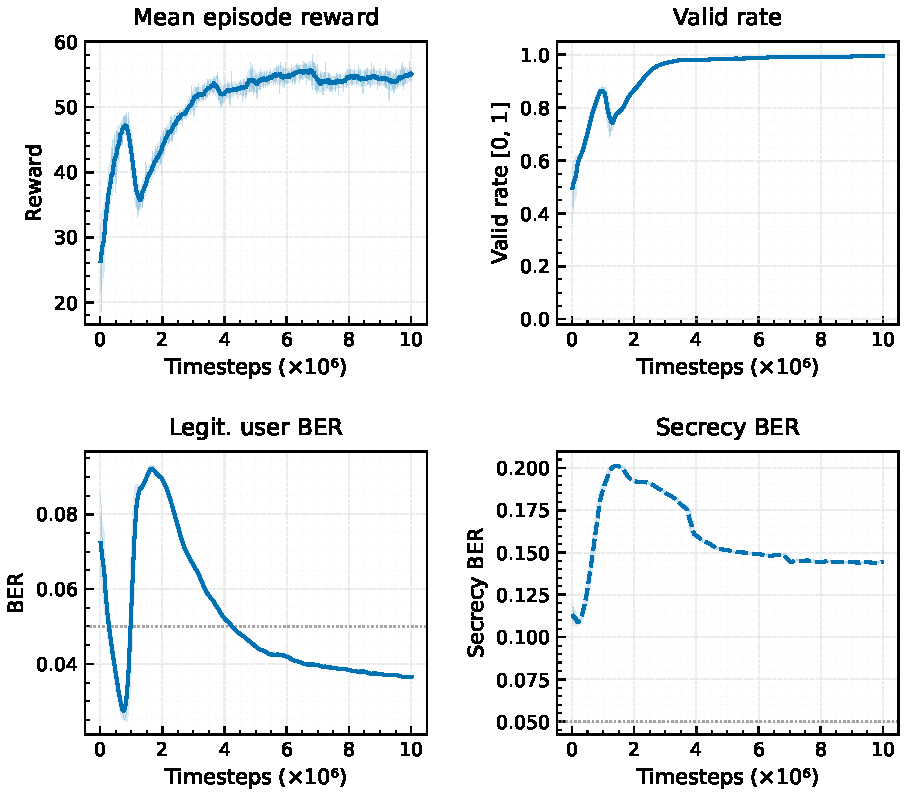
\includegraphics[width=1\textwidth]{images/chapter5/overview.pdf}
    \caption{Four-panel training overview: mean episode reward, valid-action rate, legitimate user\gls{BER}, and secrecy\gls{BER}.}
    \label{fig:training_overview}
\end{figure}
\FloatBarrier

%**************************************************************
\section{Inference results}
\subsubsection{Beam pattern}

\figurename~\ref{fig:model_beam_pattern} presents the beam patterns obtained at inference for three representative target angles: $\varphi^* \in \{-60\degree, 0\degree, 60\degree\}$, as described in the plot legend. In each case the solid line corresponds to the deterministic solution (\texttt{deterministic=True}), representing the policy mean $\mu_\theta(\varphi^*)$. All three deterministic beams exhibit a well-defined principal lobe with its peak precisely aligned to the desired angle, confirming that the policy has learned to map each target direction to a valid, high-quality beamforming configuration. \\
The transparent lines of matching color represent stochastic samples drawn from the same policy (\texttt{deterministic=False}). These samples preserve the correct pointing direction, their principal lobe peaks remain at $\varphi^*$ while exhibiting moderate sidelobe energy relative to the deterministic solution. Importantly, the amplitude loss at the main lobe is negligible across all stochastic samples, confirming that diversity is achieved without compromising the primary beamforming objective.

\begin{figure}[htbp]
    \centering
    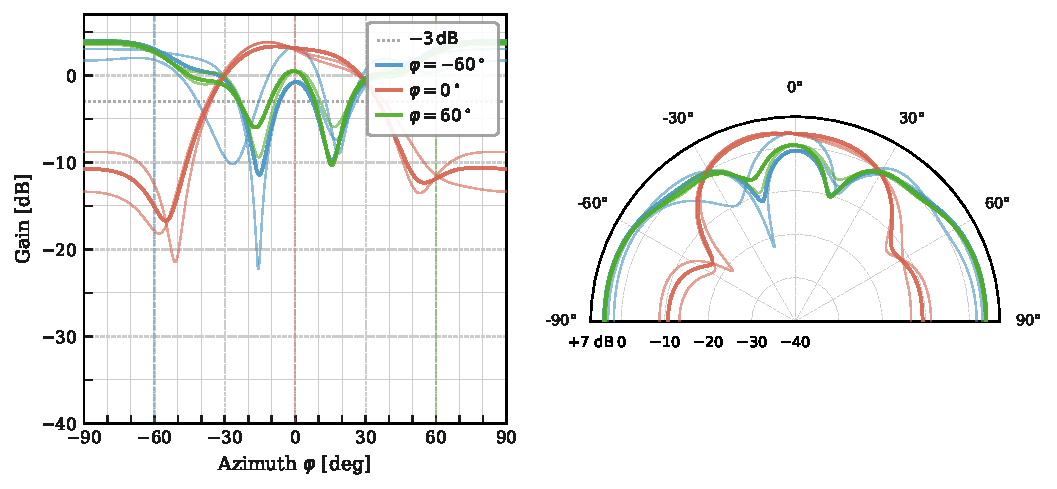
\includegraphics[width=1\textwidth]{images/chapter5/beam_pattern.pdf}
    \caption{Beam patterns produced by the trained\gls{PPO} agent for three target angles ($\varphi = -60\degree$, $0\degree$, $60\degree$). Solid lines show deterministic inference; transparent lines show stochastic samples.}
    \label{fig:model_beam_pattern}
\end{figure}
\FloatBarrier

\subsubsection{Diversity Analysis}
\label{sec:diversity_analysis}
\figurename~\ref{fig:model_diversity_analysis} reports the outcome of 100 stochastic inference draws at each integer target angle $\varphi^* \in [-90\degree, 90\degree]$, for a total of 18{,}100 samples. Each bar is decomposed into three categories: unique valid configurations (blue), duplicate solutions, and failed configurations that violated the amplitude or phase constraints (red). \\
The results confirm the robustness of the trained policy across the full angular range. Of all samples, 18{,}072 (99.8\%) are unique valid configurations, 27 (0.1\%) are duplicates, and only 1 (0.0\%) is a failure, demonstrating that the policy reliably explores distinct regions of the solution manifold rather than collapsing onto a single solution. \\
The sole systematic deviation from perfect diversity is a mild concentration of duplicate samples in the broadside region ($\varphi^* \in [-9\degree, 9\degree]$). Outside this region, duplicates are negligible and failures are absent across the entire angular range.

\begin{figure}[htbp]
    \centering
    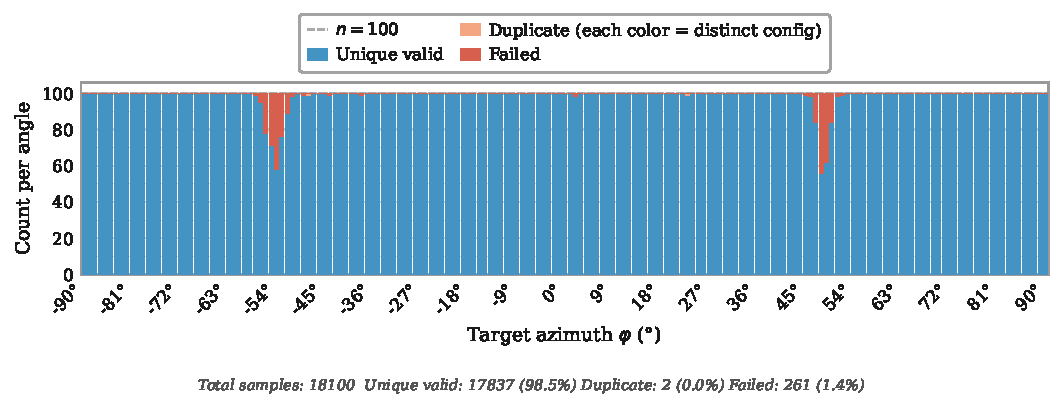
\includegraphics[width=1\textwidth]{images/chapter5/diversity_analysis.pdf}
    \caption{Outcome of 100 stochastic inference draws at each integer target angle $\varphi^* \in [-90\degree, 90\degree]$, for a total of 18{,}100 samples. Each bar is decomposed into three categories: unique valid configurations (blue), duplicate solutions (orange), and failed configurations that violated the amplitude or phase constraints (red).}
    \label{fig:model_diversity_analysis}
\end{figure}
\FloatBarrier

\subsubsection{Bit Error Rate \& Symbol Error Rate}

\figurename~\ref{fig:model_ber_ser_ebn0} presents the\gls{SER} and\gls{BER} curves obtained for $M$-\gls{PSK} modulation orders $M \in \{2, 4, 8, 16\}$, at target angle $\varphi = 30\degree$ with a $N = 5$ element\gls{ULA}. For each modulation order, $K = 5$ stochastic beamforming configurations are sampled from the trained policy, producing the thin solid curves, whose spread directly reflects the diversity of valid solutions explored by the agent. The dashed curves represent the theoretical baseline assuming a perfect array gain equal to $N$, serving as an upper bound on achievable performance.\\
Two observations are immediate. First, the simulated curves are consistently shifted to the right of their theoretical counterparts across all modulation orders; This gap is a direct consequence of the stochastic beamforming policy: unlike a deterministic matched filter, the sampled configurations do not maximize array gain at every draw, instead trading peak performance for solution diversity and secrecy. Second, the spread among the $K=5$ curves per modulation order is non-negligible, particularly for higher $M$, confirming that distinct stochastic samples produce meaningfully different received $E_b/N_0$ conditions.\\
These results should be interpreted in the context of the present work's primary objective. The proposed framework is not intended as a production-ready beamformer optimized for link budget, but as a foundational demonstration that a\gls{RL} agent can learn to navigate the directional modulation solution manifold and produce valid, diverse configurations.

\begin{figure}[htbp]
    \centering
    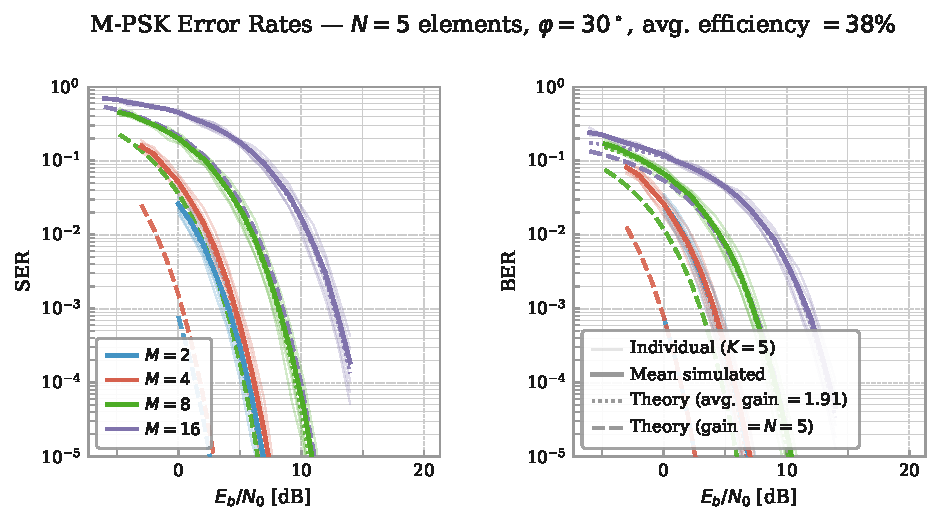
\includegraphics[width=1\textwidth]{images/chapter5/ber_ser_ebn0.pdf}
    \caption{\gls{SER} and\gls{BER} curves obtained for $M$-\gls{PSK} modulation orders $M \in \{2, 4, 8, 16\}$, at target angle $\varphi = 30\degree$ with a $N = 5$ element\gls{ULA}.}
    \label{fig:model_ber_ser_ebn0}
\end{figure}
\FloatBarrier



\subsubsection{Constellation}

\figurename~\ref{fig:model_constellations} illustrate the relationship between array gain, modulation order, and noise margin. Symbol error rates are estimated over 50,000 Monte Carlo trials per modulation scheme.
At $M = 2$ (BPSK), performance is near-perfect: the two symbol clouds are well-separated and entirely contained within their respective decision regions, yielding\gls{BER} $= 0.000$. The system operates comfortably above the noise floor despite the sub-ideal array gain, confirming that BPSK is robust to the gain loss introduced by stochastic beamforming. At $M = 4$ (QPSK), the constellation remains largely correct, with only isolated error points visible near decision boundaries, indicating that the inter-symbol distance is still sufficient at this SNR.
The picture degrades substantially at $M = 8$, where the reduced angular separation between symbols ($45\degree$) brings the noise clouds into contact with adjacent decision regions, producing a\gls{BER} of $1.4 \times 10^{-2}$. While individual symbol clusters are still discernible, a non-negligible fraction of received points cross decision boundaries, particularly for symbols in close angular proximity. At $M = 16$, the system experiences catastrophic failure (SER $= 2.1\times10^{-1}$): the $22.5\degree$ inter-symbol spacing is irreconcilable with the noise variance induced by the limited array gain, and the received point cloud is almost uniformly distributed across decision regions, rendering reliable demodulation impossible at this SNR.\\
These results establish a clear operating boundary for the proposed beamforming framework: modulation orders up to $M = 4$ are reliably supported at $E_s/N_0 = 10$~dB given the current array configuration and gain efficiency. Higher-order modulation would require either a larger array to recover gain, a higher operating SNR, or improvements on the gain-aware reward signal during training to steer the policy toward configurations that better preserve array gain.

\begin{figure}[htbp]
    \centering
    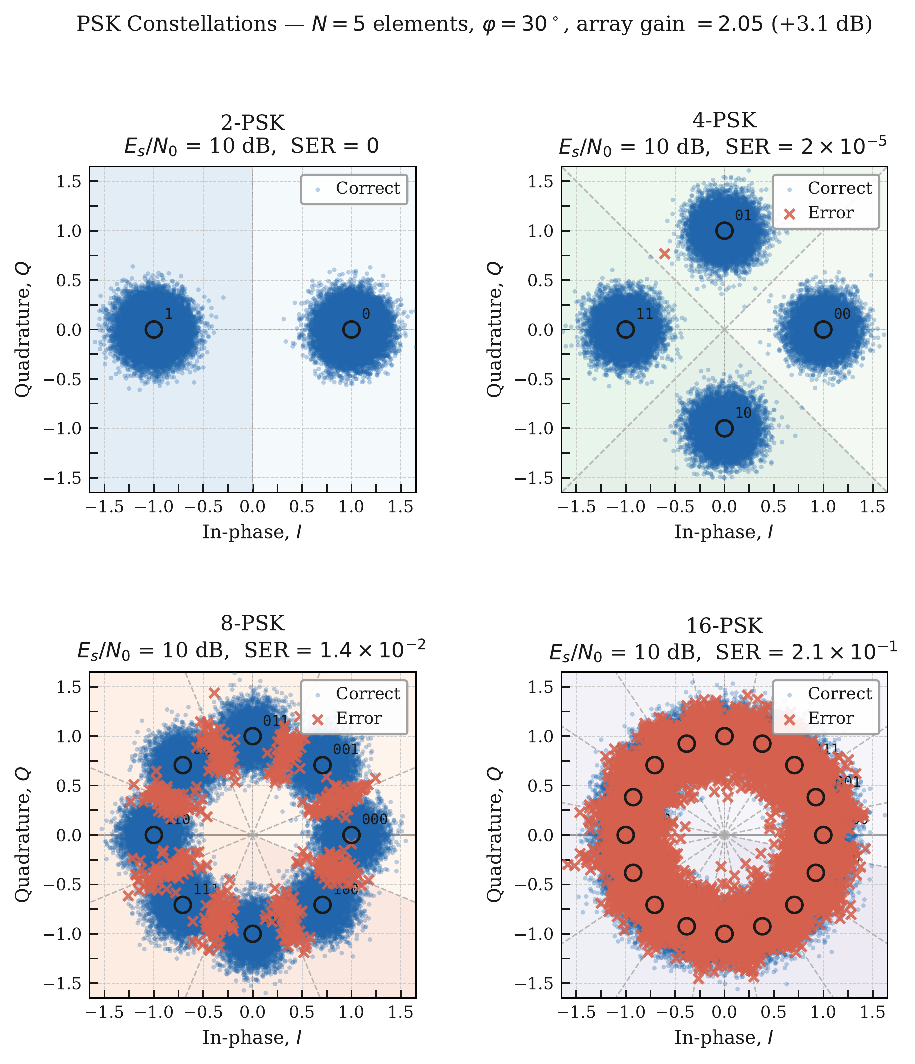
\includegraphics[width=1\textwidth]{images/chapter5/constellations.pdf}
    \caption{IQ constellations for $M$-PSK modulation at $E_s/N_0 = 10$~dB with $N=5$ elements at $\varphi = 30\degree$. Blue dots indicate correct detections; red crosses indicate symbol errors. Open circles mark ideal symbol positions with Gray-coded bit labels.}
    \label{fig:model_constellations}
\end{figure}
\FloatBarrier

\subsubsection{SER vs.\ Angle}

\figurename~\ref{fig:ser_vs_angle} shows the\gls{SER} as a function of azimuth angle at a fixed $E_s/N_0 = 10$~dB, with the legitimate user steered to $\varphi = 30\degree$. A well-trained beamforming policy should maintain low error rates in the targeted direction while exhibiting high error rates elsewhere, indicating signal distortion outside the intended direction. In our plot it can be observed that the best angle for eavesdroppers are those that are physically near the legittimate receiver and the further away the eavesdropper is, the greater the error rate.

\begin{figure}[htbp]
    \centering
    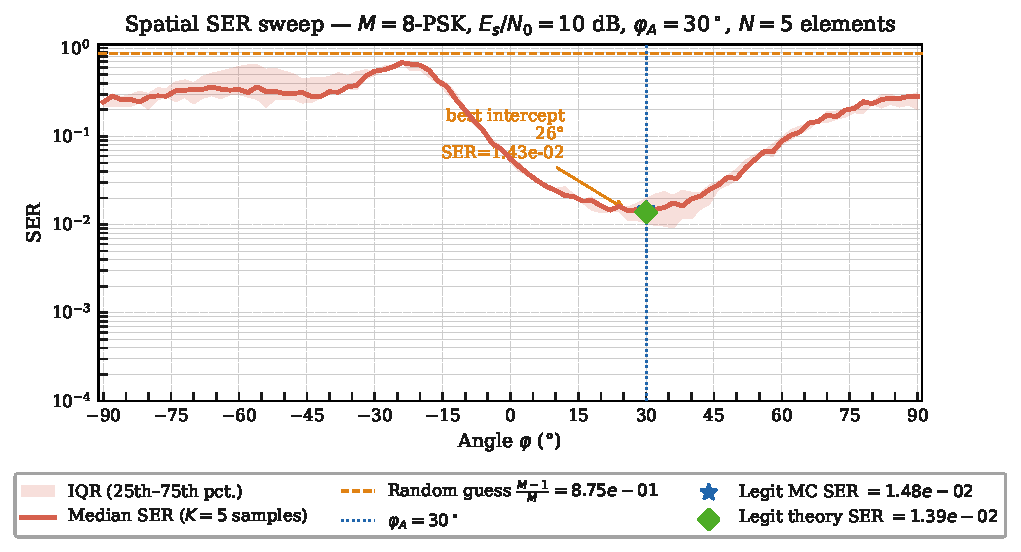
\includegraphics[width=1\textwidth]{images/chapter5/ser_vs_angle.pdf}
    \caption{SER as a function of azimuth angle at fixed $E_s/N_0 = 10$~dB, with the legitimate user steered to $\varphi = 30\degree$.}
    \label{fig:ser_vs_angle}
\end{figure}
\FloatBarrier

\figurename~\ref{fig:secrecy_matrix} presents a more generalized view of the physical-layer security: the secrecy matrix obtained by evaluating the\gls{BER} over a grid of legitimate and eavesdropper angles at fixed $E_s/N_0 = 10$~dB. For each pair $(\varphi_\mathrm{Bob}, \varphi_\mathrm{Eve})$, the matrix reports the channel secrecy of the configuration. It can be observed that, as shown along the center diagonal, the closer the eavesdropper is to the target angle the lower the channel secrecy.

\begin{figure}[htbp]
    \centering
    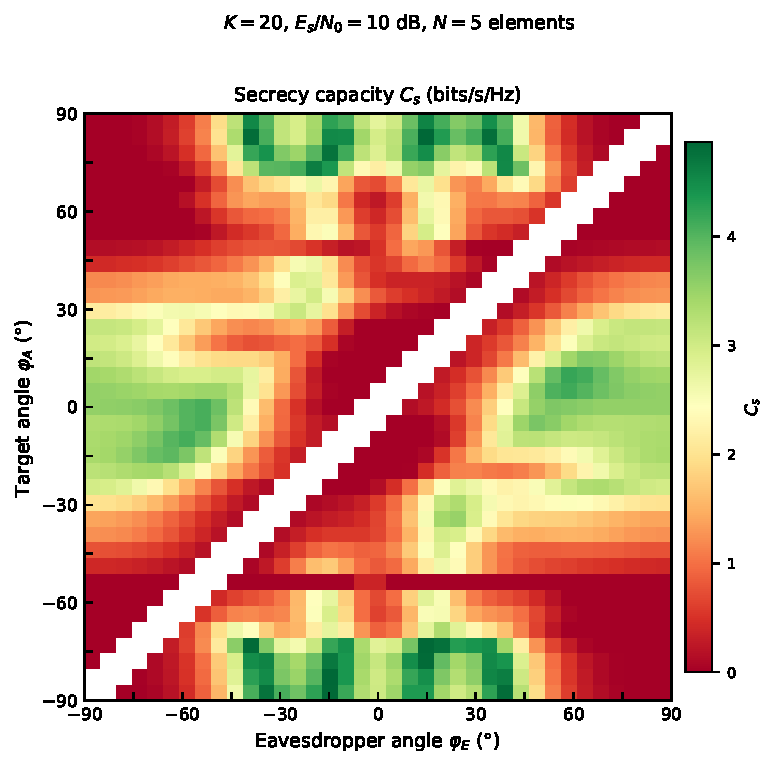
\includegraphics[width=1\textwidth]{images/chapter5/secrecy_matrix.pdf}
    \caption{Secrecy matrix:\gls{BER} evaluated over a grid of legitimate-user and eavesdropper angles at fixed $E_s/N_0 = 10$~dB.}
    \label{fig:secrecy_matrix}
\end{figure}
\FloatBarrier

\subsubsection{Amplitude Profile}

\figurename~\ref{fig:amplitude_profile} illustrates the amplitude weights of the antenna elements produced by the trained policy throughout the full angular range $\varphi \in [-90\degree, 90\degree]$. For each target angle, $K = 5$ stochastic samples are drawn from the policy and the resulting amplitude profiles are superimposed. This figure reveals how the agent allocates power across the array elements as a function of steering direction, revealing that near angles in which the phase constraints become harder to satisfy (\subsectionname~\ref{subsec:angle_dependant_constraint}) the model will allocate less amplitude or none at all to specific elements in order to reduce the complexity.

\begin{figure}[htbp]
    \centering
    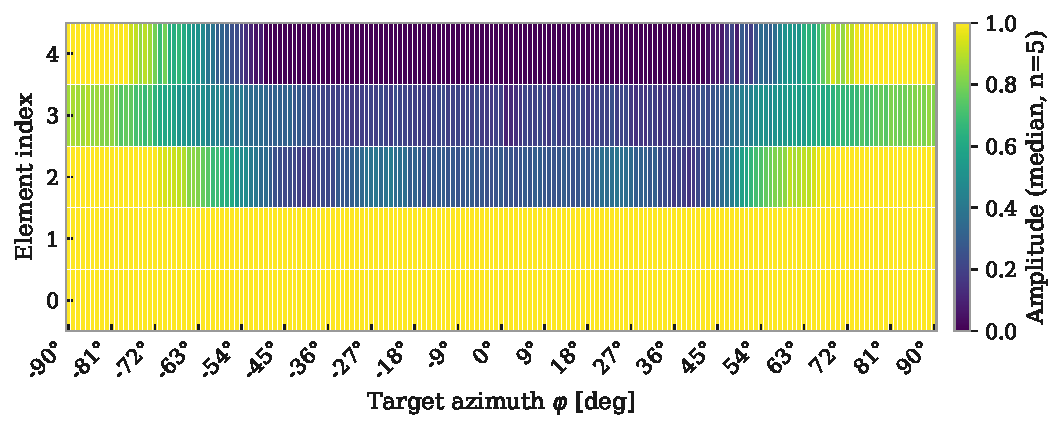
\includegraphics[width=1\textwidth]{images/chapter5/amplitude_profile.pdf}
    \caption{Antenna element amplitude weights produced by the trained\gls{PPO} policy across target angles $\varphi \in [-90\degree, 90\degree]$, with $K=5$ stochastic samples per angle.}
    \label{fig:amplitude_profile}
\end{figure}
\FloatBarrier

%**************************************************************
\section{Comparison with Random Search}
\label{sec:benchmark}

This section benchmarks the trained\gls{PPO} model against a two baselines:
\begin{itemize}
    \item a naive random phase search;
    \item\gls{CEM}, a population-based stochastic optimization approach.
\end{itemize}
For each azimuth angle $\varphi \in [-90\degree, 90\degree]$, all three methods are tasked with finding a valid beamforming configuration that satisfies the amplitude floor and phase flatness constraints used during training. The random search draws uniform random phases from $[0, 2\pi)^N$ until a valid configuration is found or a maximum of $10{,}000$ attempts is exhausted;\gls{CEM} iteratively refines a sampling distribution over phase configurations by fitting to the best-performing samples from each generation, validating candidates as they are drawn; the\gls{PPO} model draws stochastic samples from the trained policy and validates each one in turn, stopping at the first valid draw or after $500$ attempts.

\subsection{Sample Efficiency}

\figurename~\ref{fig:benchmark_efficiency} compares the three methods in terms of the number of candidates evaluated before a valid solution is found (left panel) and the success rate across angles (right panel). Solid lines report the median number of tries, with shaded bands covering the 25th--75th percentile range across independent repetitions. The\gls{PPO} model requires substantially fewer candidates to find a valid configuration at most angles.\gls{CEM} improves on naive random search by adapting its sampling distribution over successive generations, but still requires considerably more candidates as it lacks any prior knowledge of the constraint structure. The naive random approach takes the shape of a gaussian distribution with the broadside angles requiring more tries, a trend similar to\gls{CEM} sice it is initialized from a similarly uniformed distribution.
\begin{figure}[htbp]
    \centering
    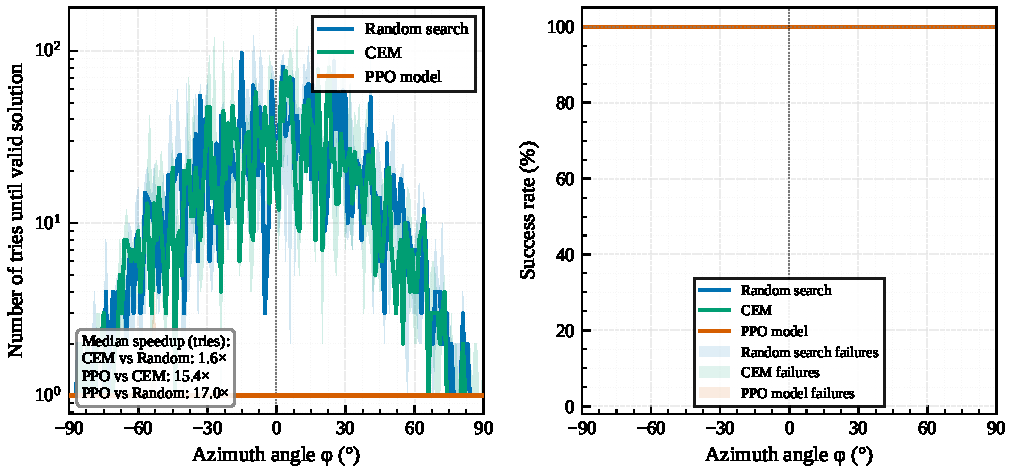
\includegraphics[width=0.8\textwidth]{images/chapter5/benchmark_efficiency.pdf}
    \caption{Sample efficiency comparison between\gls{PPO} model,\gls{CEM}, and random search: number of tries to find a valid configuration (left) and success rate across angles (right). Shaded bands show the 25th-75th percentile range.}
    \label{fig:benchmark_efficiency}
\end{figure}
\FloatBarrier

\subsection{Search Latency}

\figurename~\ref{fig:benchmark_latency} reports the total wall-clock latency (in milliseconds) required to find a valid beamforming configuration for each azimuth angle. The median latency annotations in the figure quantify the practical speed advantage of the learned policy over both baselines: the median latency is $0.3ms$ for the learned policy, $0.7ms$ for\gls{CEM} and $2.1ms$ for random search. These results indicate that, altough\gls{CEM}'s adaptive sampling offers a modest efficiency gain over a purely random strategy, it does not approach the latency reduction afforded by the learned policy.
\\
\\
It is worth noting that this comparison, while informative of raw search efficiency, is not entirely like-for-like: random search and\gls{CEM} are only tasked with satisfying the amplitude floor and phase flatness constraints, whereas the\gls{PPO} model is trained under an objective that additionally rewards configurations which degrade the\gls{SNR} at potential eavesdropper locations. The speedup and sample efficiency gains reported above therefore likely understate the relative advantage of the learned policy, which must satisfy a strictly harder, multi-objective problem within the same or fewer search attempts.

\begin{figure}[htbp]
    \centering
    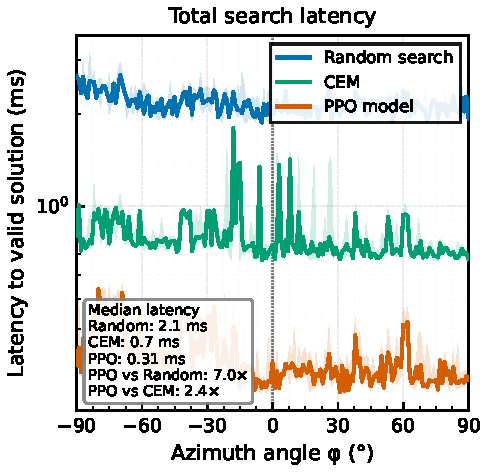
\includegraphics[width=0.6\textwidth]{images/chapter5/benchmark_latency.pdf}
    \caption{Total latency (ms) to find a valid beamforming configuration:\gls{PPO} model vs.\\gls{CEM} vs.\ random search across all azimuth angles. Shaded bands show the 25th--75th percentile range.}
    \label{fig:benchmark_latency}
\end{figure}
\FloatBarrier

\section{Training variation}

The three experiments presented in this section explore modifications to the baseline $N=5$ system:
\begin{enumerate}
    \item flattens the curriculum, making the model face the final constraints from the very beginning;
    \item replaces the raw phase parameterisation with a physics-informed action parameterisation;
    \item builds on the second experiment by also scaling the array to $N=8$ elements.
\end{enumerate}

\subsection{Curriculum Learning flattened}
\label{subsec:curriculum_flattened}
\subsubsection{Results}

Removing the curriculum-learning stages and training directly under the full set of constraints leads to a clear degradation in performance: the learned policy fails to exploit the amplitude degrees of freedom available to the array and instead converges to solutions where nearly all antenna elements operate at maximum amplitude. In contrast to the curriculum-trained model, no meaningful power allocation strategy emerges, indicating that the optimisation problem becomes substantially harder when the agent is exposed to the complete constraint set from the beginning of training. This behaviour has a direct impact on secrecy performance, rendering the policy unable to learn to selectively attenuate individual elements, losing one of the few mechanisms available for shaping the array response beyond the constrained phase parameterisation. As a result, secrecy is largely neglected during optimisation and the resulting solutions exhibit significantly poorer secrecy characteristics than those obtained with the staged curriculum approach.
\\
\\
Analysis of 100 stochastic inference draws shows that the flattened-curriculum model produces consistently worse validation performance and completely fails for several receiver positions where the curriculum-trained policy remains robust. It can also be observed that the standard deviation of the validation metric remains higher throughout training and increases towards the final stages. Although the flattened-curriculum model ultimately converges to a valid policy, the final solution is markedly less stable, generalises poorly, and achieves substantially worse overall performance than the curriculum-based approach.

\begin{figure}[p]  % Force to its own page
    \centering
    \begin{subfigure}{\textwidth}
        \centering
        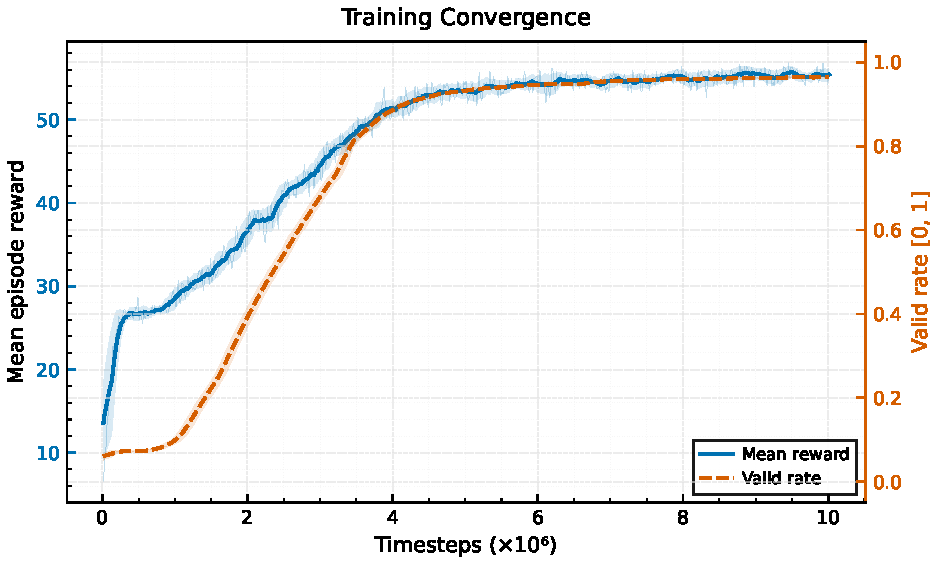
\includegraphics[width=0.8\textwidth]{images/chapter5/no_curriculum/training_convergence.pdf}
        \caption{Mean episode reward and valid-action rate}
        \label{fig:no_curriculum_training_convergence}
    \end{subfigure}
    
    \vspace{5pt}
    
    \begin{subfigure}{\textwidth}
        \centering
        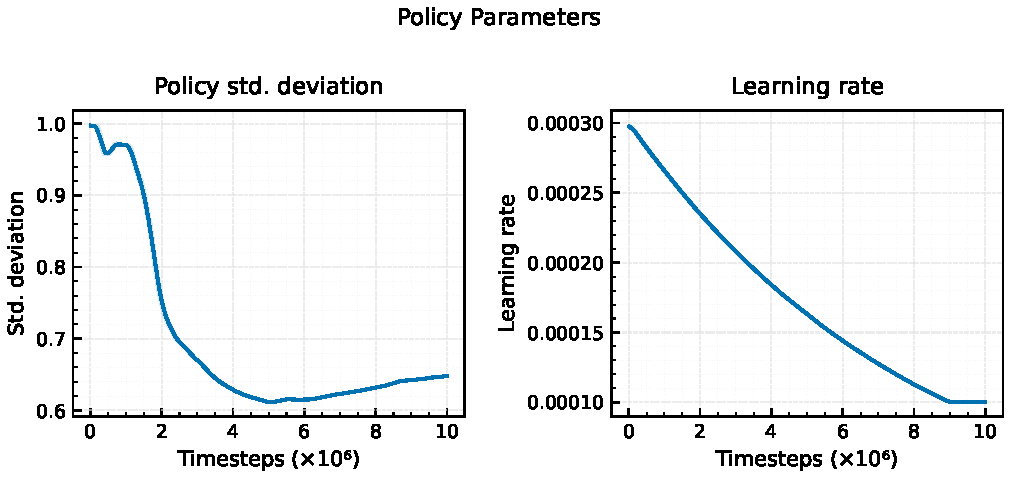
\includegraphics[width=0.8\textwidth]{images/chapter5/no_curriculum/policy_parameters.pdf}
        \caption{Action standard deviation and learning rate}
        \label{fig:no_curriculum_training_params}
    \end{subfigure}
    
    \vspace{5pt}
    
    \begin{subfigure}{\textwidth}
        \centering
        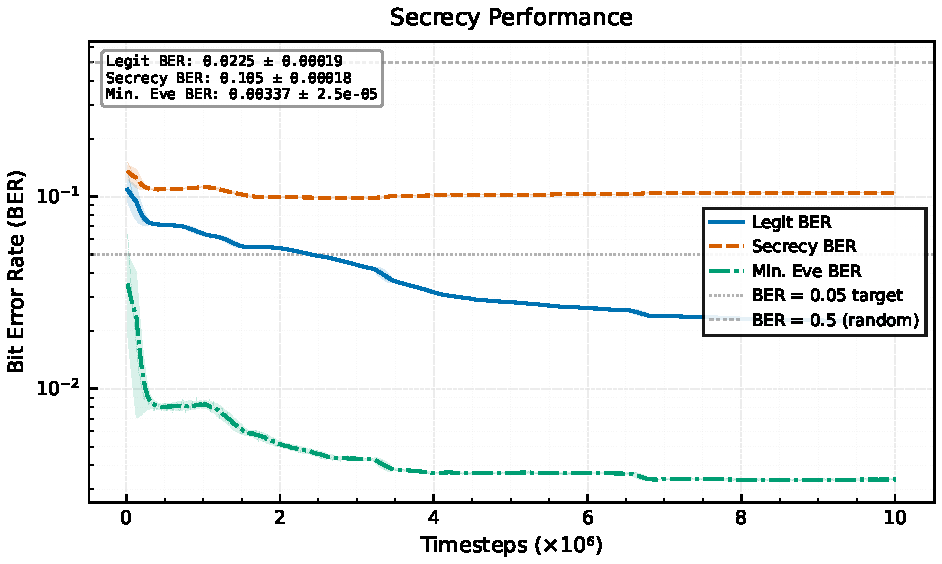
\includegraphics[width=0.8\textwidth]{images/chapter5/no_curriculum/secrecy_performance.pdf}
        \caption{BER metrics (legitimate user, secrecy, and minimum eavesdropper)}
        \label{fig:no_curriculum_training_ber}
    \end{subfigure}
    
    \caption{Training overview for the curriculum flattened $N=5$\gls{ULA}. Top: mean episode reward and valid-action rate. Middle: action standard deviation and learning rate. Bottom:\gls{BER} metrics (legitimate user, secrecy, and minimum eavesdropper).}
    \label{fig:no_curriculum_training}
\end{figure}

\begin{figure}[htbp]
    \centering
    \begin{minipage}[t]{0.49\textwidth}
        \centering
        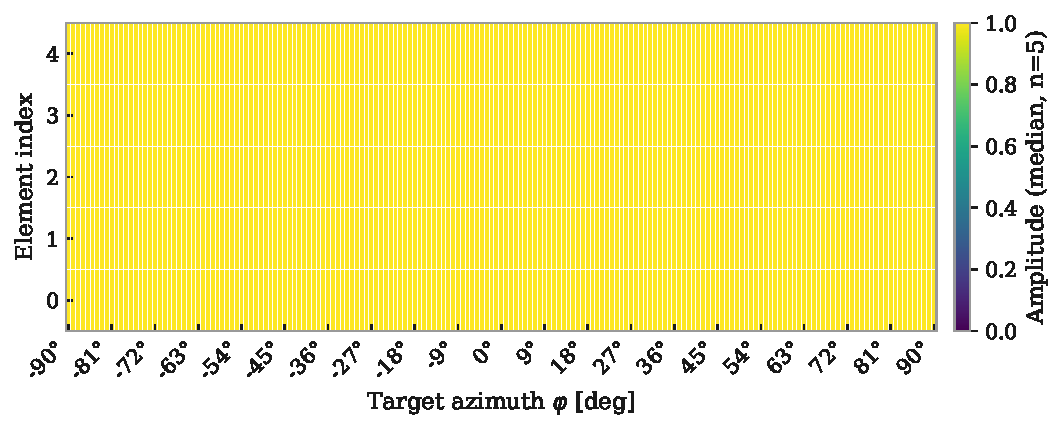
\includegraphics[width=\linewidth]{images/chapter5/no_curriculum/amplitude_profile.pdf}
    \end{minipage}\hfill
    \begin{minipage}[t]{0.49\textwidth}
        \centering
        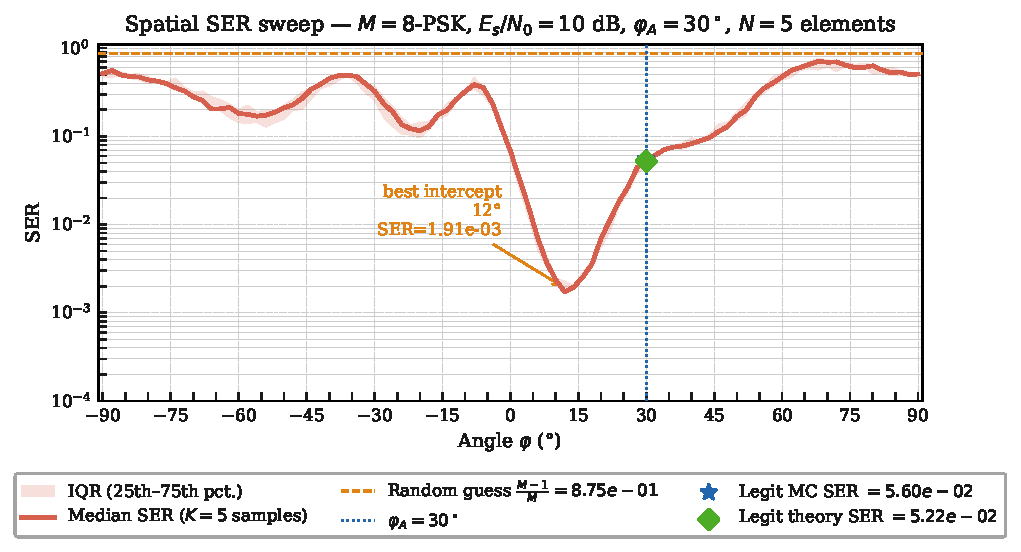
\includegraphics[width=\linewidth]{images/chapter5/no_curriculum/ser_vs_angle.pdf}
    \end{minipage}\\[4pt]
    \begin{minipage}[t]{0.49\textwidth}
        \centering
        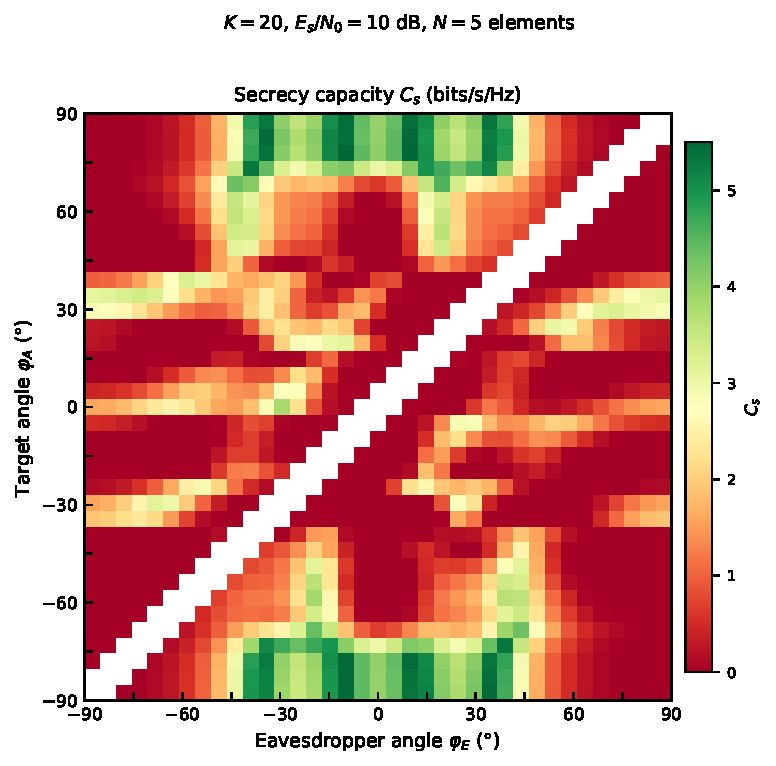
\includegraphics[width=\linewidth]{images/chapter5/no_curriculum/secrecy_matrix.pdf}
    \end{minipage}\hfill
    \begin{minipage}[t]{0.49\textwidth}
        \centering
        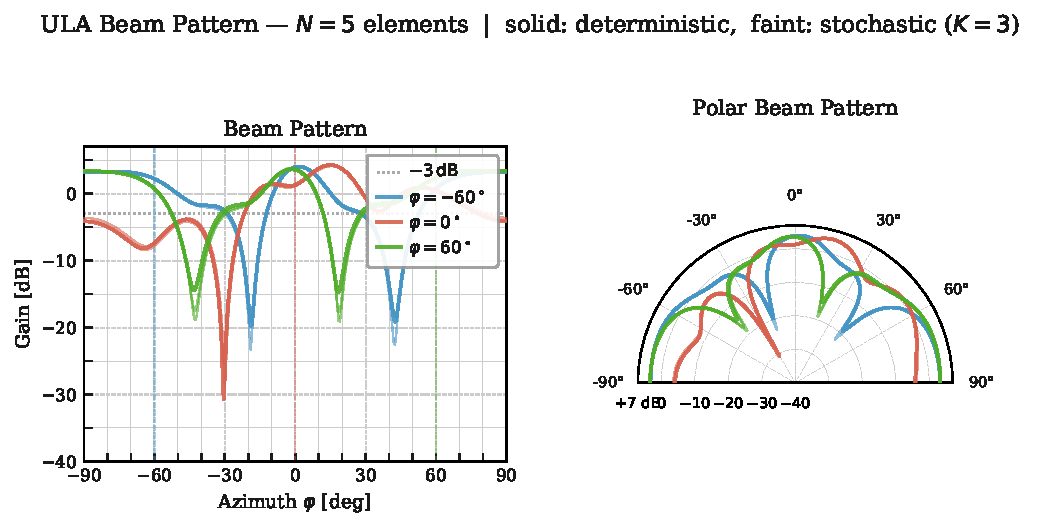
\includegraphics[width=\linewidth]{images/chapter5/no_curriculum/beam_pattern.pdf}
    \end{minipage}
    \caption{Inference overview for the curriculum flattened $N=5$\gls{ULA}. Top-left: amplitude profile across the full angular range.. Top-right:\gls{BER} vs.\ azimuth angle at $E_s/N_0 = 10$\,dB with the legitimate user at $\varphi = 30\degree$. Bottom-left: secrecy matrix. Bottom-right: beam patterns for $\varphi \in \{-60\degree, 0\degree, 60\degree\}$}
    \label{fig:no_curriculum_inference}
\end{figure}

\begin{figure}[htbp]
    \centering
    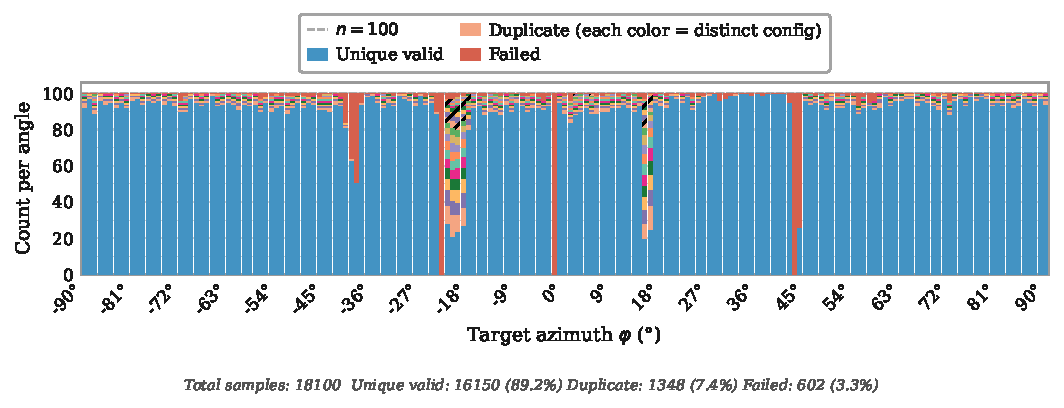
\includegraphics[width=1.0\textwidth]{images/chapter5/no_curriculum/diversity_analysis.pdf}
    \caption{Outcome of 100 stochastic inference draws at each integer target angle $\varphi^* \in [-90\degree, 90\degree]$, for a total of 18{,}100 samples for curriculum flattened model with\gls{ULA} with $N=5$ elements. Each bar is decomposed into three categories: unique valid configurations (blue), duplicate solutions, and failed configurations that violated the amplitude or phase constraints (red).}
    \label{fig:no_curriculum_diversity_analysis}
\end{figure}
\FloatBarrier

\subsection{Physics-informed action parameterisation}

\label{subsec:physics_informed}

In the baseline formulation the agent outputs $N$ independent phase values mapped uniformly to $[0, 2\pi)$, requiring it to discover solutions through reward signal alone. The physics-informed action parameterisation removes this burden by embedding the known analytical solution directly into the action decoder. For a\gls{ULA} with elements along the $y$-axis at spacing $d$, the optimal phase increment per element for steering to azimuth $\varphi$ is:
\begin{equation}
    \Delta\varphi = \frac{2\pi}{\lambda}\,d\,\sin\varphi
\end{equation}
Instead of predicting the $N$ phases directly, the agent predicts corrections on top of this:
\begin{equation}
    \varphi_n = n\!\left(\Delta\varphi + a_0\,\sigma_s\right) + a_n\,\sigma_p \qquad n \geq 1
\end{equation}
where $a_0$ is a slope-correction action with scale $\sigma_s = \pi/4$, meaning a unit action shifts the inter-element phase increment by $\pi/4$\,rad, and $a_n$ are per-element perturbations with scale $\sigma_p = \pi/4$\,rad. Element $0$ is the phase reference and the action space dimension remains $2N$.
\figurename~\ref{fig:physics_informed_inference} and \figurename~\ref{fig:diversity_analysis_physics_informed} summarizes the inference behaviour while \figurename~\ref{fig:physics_informed_training} summarize the training dynamics.

\subsubsection{Results}
The training dynamics are stable and broadly similar to the baseline while the expressive power of the parameterisation is reduced and visible in the diversity analysis (\figurename~\ref{fig:diversity_analysis_physics_informed}: the fraction of duplicate solutions is substantially higher than in the baseline, indicating that the policy converges to a narrower set of configurations. This is a structural consequence of the $\pm\frac{\pi}{4}$ perturbation bound; Valid\gls{DDM} steering vectors tend to cluster near the\gls{DFT} ramp, so the constrained action space covers the feasible region but leaves little room for structurally distinct solutions. This result is nonetheless informative, demonstrating that physics-informed parameterisation is a viable solution and that a more expressive variant could potentially close the diversity gap and rival the purely gradient-driven baseline. 

\begin{figure}[p]  % Force to its own page
    \centering
    \begin{subfigure}{\textwidth}
        \centering
        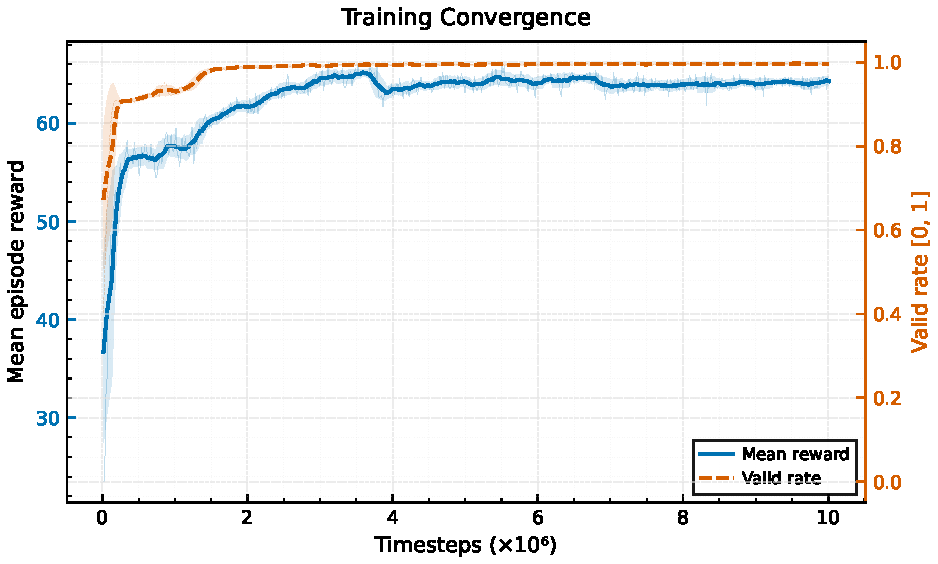
\includegraphics[width=0.8\textwidth]{images/chapter5/physics_informed/training_convergence.pdf}
        \caption{Mean episode reward and valid-action rate}
        \label{fig:physics_informed_training_convergence}
    \end{subfigure}
    
    \vspace{5pt}
    
    \begin{subfigure}{\textwidth}
        \centering
        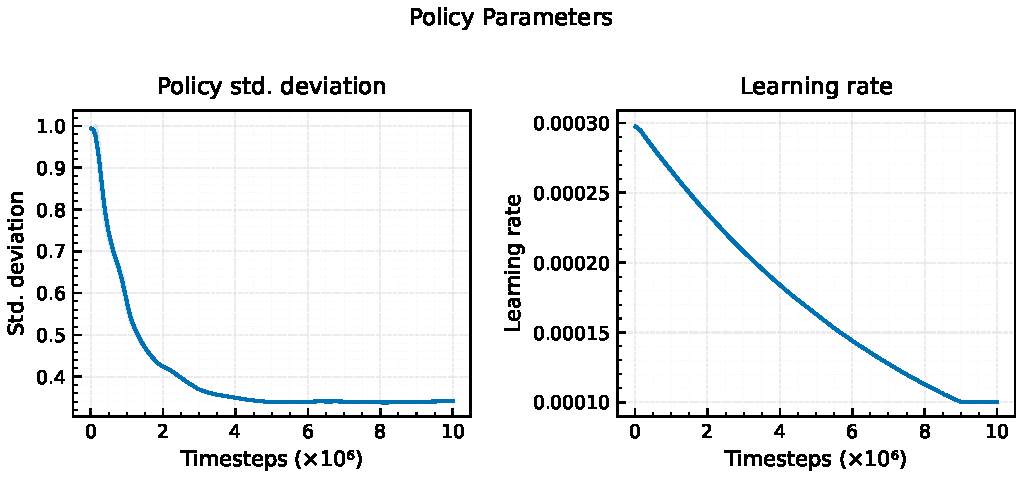
\includegraphics[width=0.8\textwidth]{images/chapter5/physics_informed/policy_parameters.pdf}
        \caption{Action standard deviation and learning rate}
        \label{fig:physics_informed_training_params}
    \end{subfigure}
    
    \vspace{5pt}
    
    \begin{subfigure}{\textwidth}
        \centering
        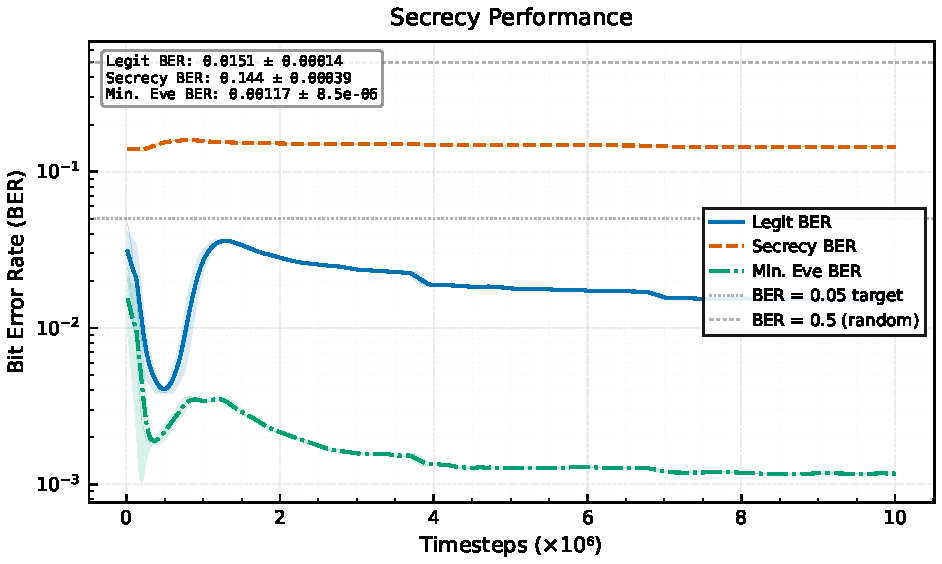
\includegraphics[width=0.8\textwidth]{images/chapter5/physics_informed/secrecy_performance.pdf}
        \caption{BER metrics (legitimate user, secrecy, and minimum eavesdropper)}
        \label{fig:physics_informed_training_ber}
    \end{subfigure}
    
    \caption{Training overview for the physics-informed action parameterisation}
    \label{fig:physics_informed_training}
\end{figure}

\begin{figure}[htbp]
    \centering
    \begin{minipage}[t]{0.49\textwidth}
        \centering
        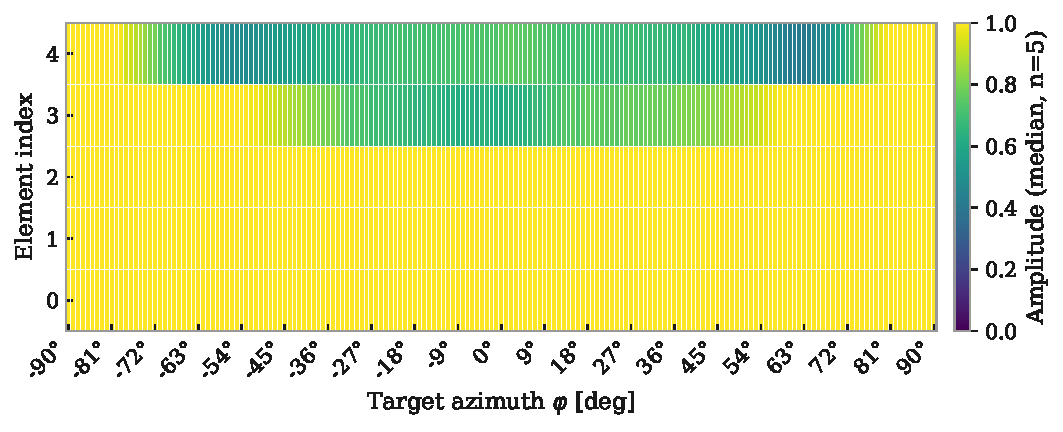
\includegraphics[width=\linewidth]{images/chapter5/physics_informed/amplitude_profile.pdf}
    \end{minipage}\hfill
    \begin{minipage}[t]{0.49\textwidth}
        \centering
        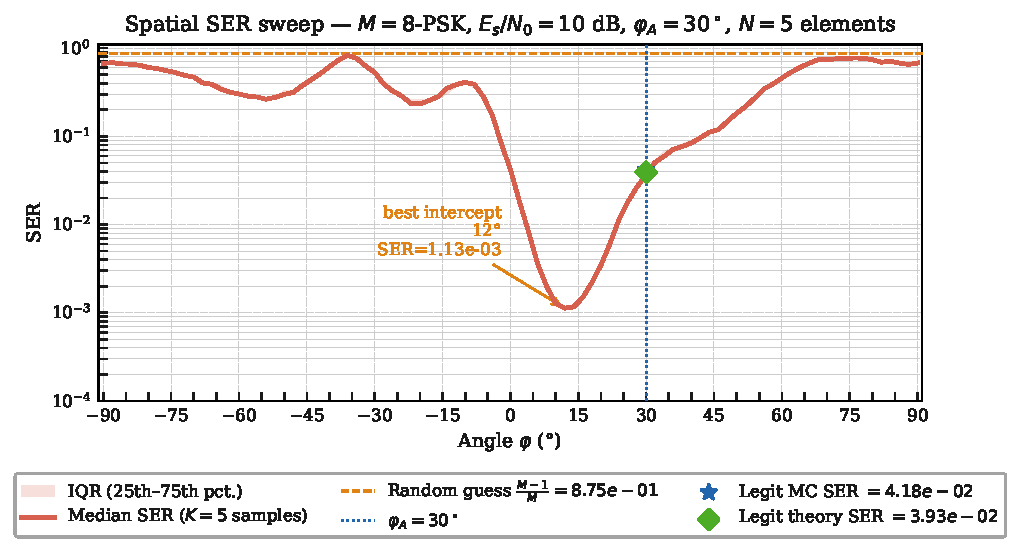
\includegraphics[width=\linewidth]{images/chapter5/physics_informed/ser_vs_angle.pdf}
    \end{minipage}\\[4pt]
    \begin{minipage}[t]{0.49\textwidth}
        \centering
        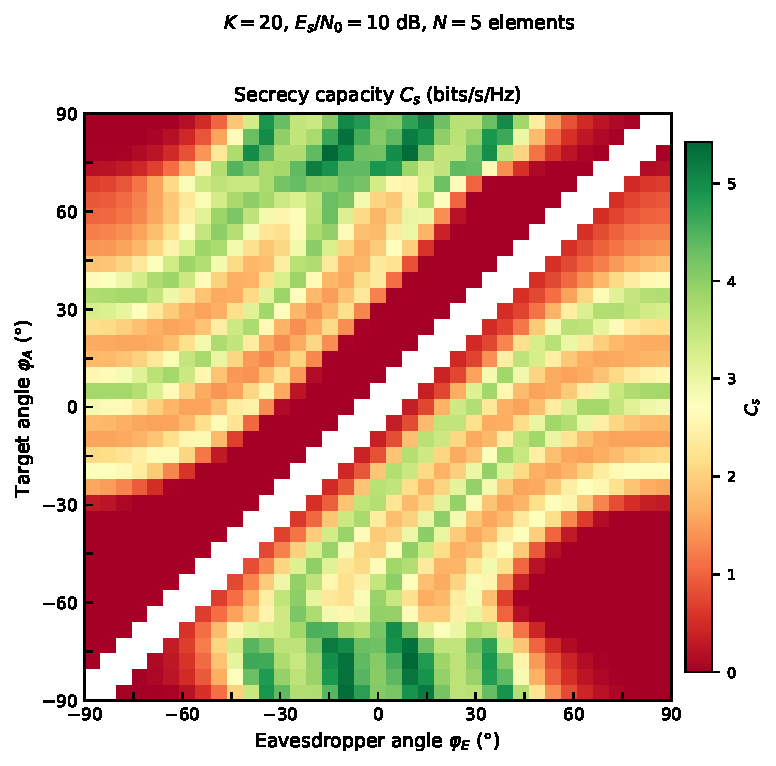
\includegraphics[width=\linewidth]{images/chapter5/physics_informed/secrecy_matrix.pdf}
    \end{minipage}\hfill
    \begin{minipage}[t]{0.49\textwidth}
        \centering
        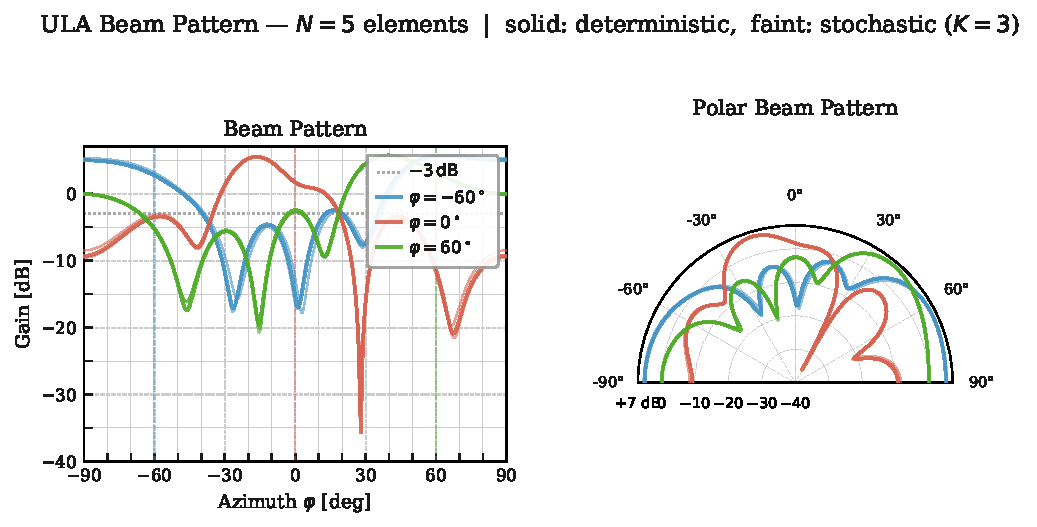
\includegraphics[width=\linewidth]{images/chapter5/physics_informed/beam_pattern.pdf}
    \end{minipage}
    \caption{Inference overview for the physics-informed action parameterisation. Top-left: amplitude profile across the full angular range. Top-right:\gls{BER} vs.\ azimuth angle at $E_s/N_0 = 10$\,dB with the legitimate user at $\varphi = 30\degree$. Bottom-left: secrecy matrix. Bottom-right: beam patterns for $\varphi \in \{-60\degree, 0\degree, 60\degree\}$.}
    \label{fig:physics_informed_inference}
\end{figure}

\begin{figure}[htbp]
    \centering
    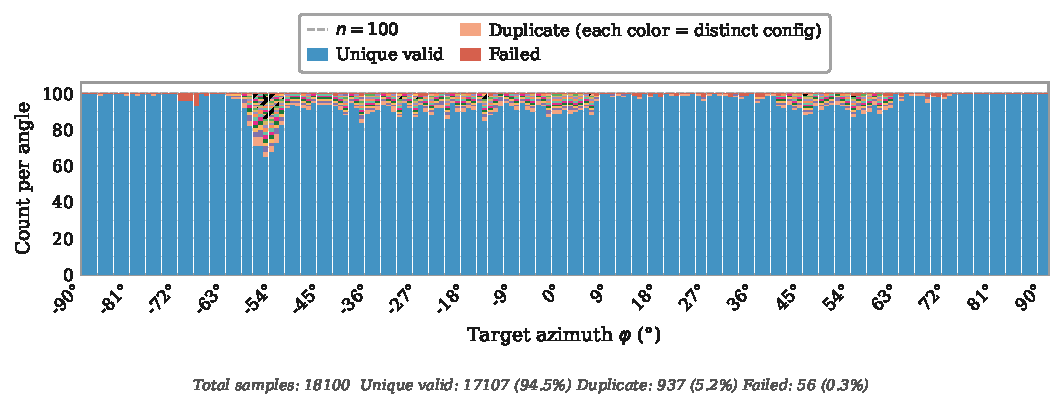
\includegraphics[width=1.0\textwidth]{images/chapter5/physics_informed/diversity_analysis.pdf}
    \caption{Outcome of 100 stochastic inference draws at each integer target angle $\varphi^* \in [-90\degree, 90\degree]$, for a total of 18{,}100 samples for the physics-informed action parameterisation. Each bar is decomposed into three categories: unique valid configurations (blue), duplicate solutions, and failed configurations that violated the amplitude or phase constraints (red).}
    \label{fig:diversity_analysis_physics_informed}
\end{figure}

\FloatBarrier

\subsection{ULA with \texorpdfstring{$N = 8$}{N = 8} elements}
\label{subsec:ula8}

Scaling from $N=5$ to $N=8$ elements introduces three compounding difficulties:
\begin{enumerate}
    \item the beamwidth narrows proportionally to $1/N$, so the fixed $\pm 5\degree$ validation window covers a larger fraction of the main lobe, making phase flatness harder to achieve;
    \item the action space grows to $2N=16$ dimensions, increasing the exploration burden and the credit-assignment difficulty per rollout;
    \item the phase of the normalised array response depends jointly on all $N$ element phases; with more elements, any inter-element misalignment produces stronger phase ripple across the support window.
\end{enumerate}
This experiment combines the physics-informed action parameterisation with a larger array, building on the results of \subsectionname~\ref{subsec:physics_informed}. All other hyperparameters, curriculum settings, and reward weights are identical to the $N=5$ baseline.

\figurename~\ref{fig:ula8_inference} and \figurename~\ref{fig:ula8_diversity_analysis} summarize the inference behavior, while \figurename~\ref{fig:ula8_training} summarizes the training dynamics.

\subsubsection{Results}
The experiment compounds the limitations identified in \subsectionname~\ref{subsec:physics_informed}. The inference results show that the physics-informed policy uses almost all elements at near-full amplitude, with at most one element slightly reduced, while the gradient-based baseline learns to silence or reduce elements. This root cause of this difference is that element silencing is only useful for\gls{DDM} secrecy when combined with non-ramp-like  phases; The gradient approach is free to pair reduced element amplitudes with unconventional phase assignments on the remaining elements, breaking the symmetry of the array response in a way that produces rapid phase variation outside the legitimate receiver's window. Under the physics-informed parameterisation, phases are constrained to stay within $\pm\frac{\pi}{4}$ of the\gls{DFT} ramp and silencing an element merely weakens and broadens the beam without generating the spatial phase variation that secrecy requires; The policy therefore correctly concludes that silencing is not worth the amplitude penalty since it gains nothing in secrecy. The diversity analysis (\figurename~\ref{fig:ula8_diversity_analysis}) shows that the duplicate rate is substantially higher than for $N=5$ and is distributed over the full angular range.

\begin{figure}[p]  % Force to its own page
    \centering
    \begin{subfigure}{\textwidth}
        \centering
        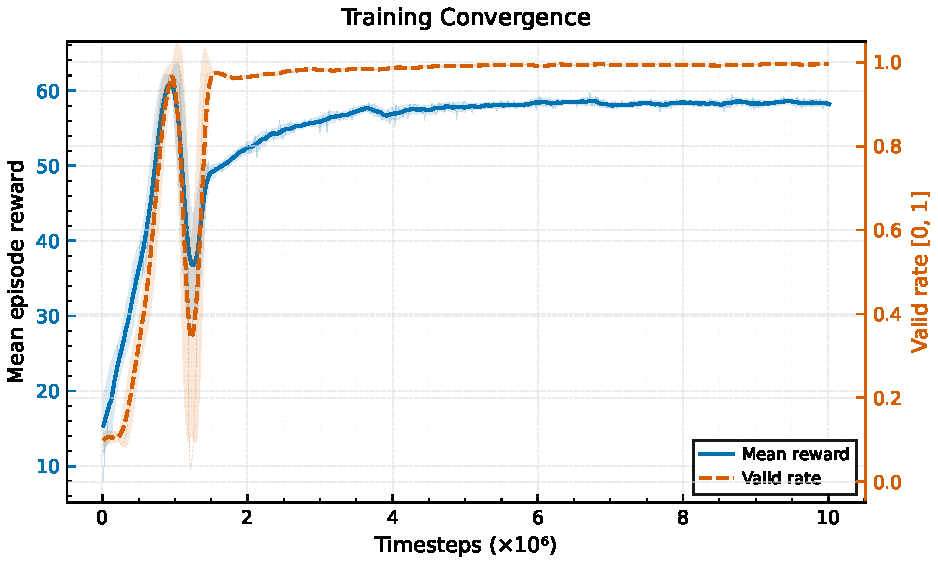
\includegraphics[width=0.8\textwidth]{images/chapter5/ula8/training_convergence.pdf}
        \caption{Mean episode reward and valid-action rate}
        \label{fig:ula8_training_convergence}
    \end{subfigure}
    
    \vspace{5pt}
    
    \begin{subfigure}{\textwidth}
        \centering
        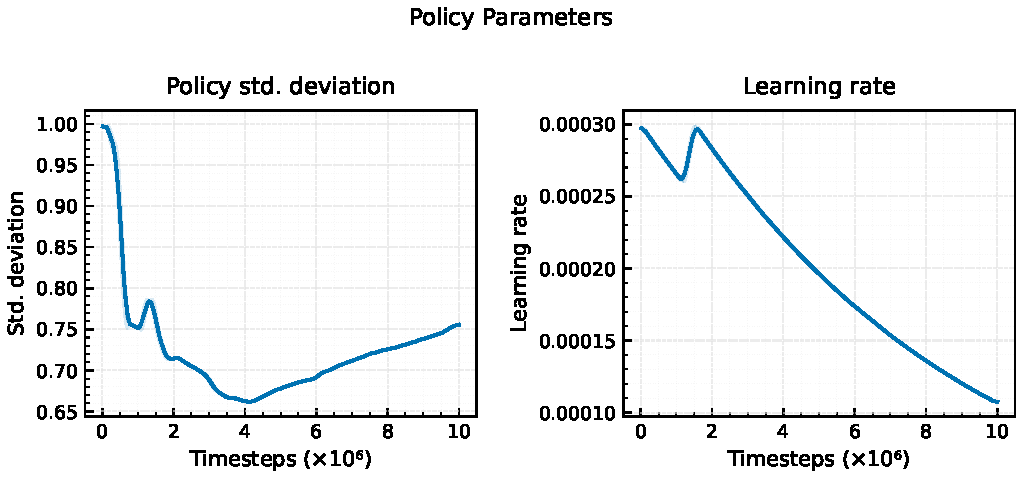
\includegraphics[width=0.8\textwidth]{images/chapter5/ula8/policy_parameters.pdf}
        \caption{Action standard deviation and learning rate}
        \label{fig:ula8_training_params}
    \end{subfigure}
    
    \vspace{5pt}
    
    \begin{subfigure}{\textwidth}
        \centering
        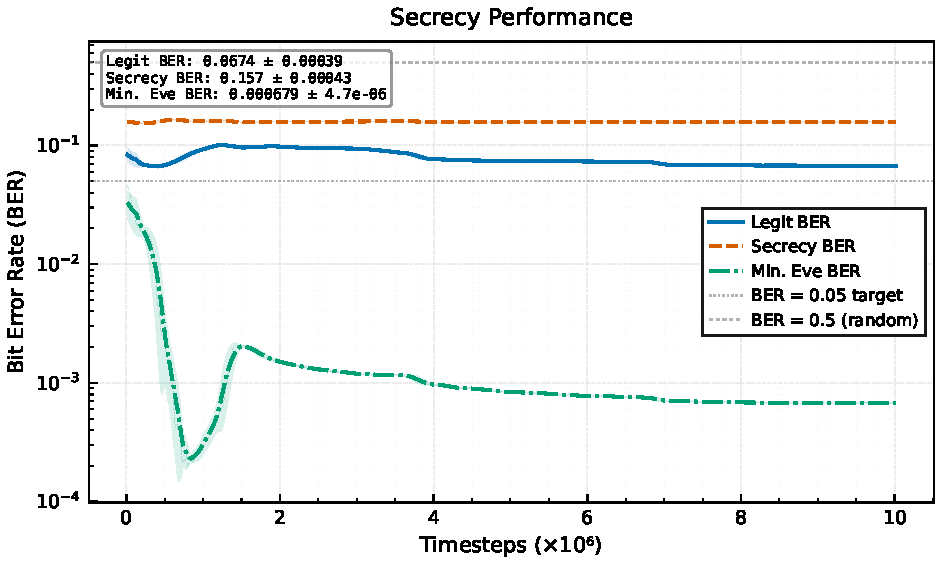
\includegraphics[width=0.8\textwidth]{images/chapter5/ula8/secrecy_performance.pdf}
        \caption{BER metrics (legitimate user, secrecy, and minimum eavesdropper)}
        \label{fig:ula8_training_ber}
    \end{subfigure}
    
    \caption{Training overview for the $N=8$\gls{ULA}. Top: mean episode reward and valid-action rate. Middle: action standard deviation and learning rate. Bottom:\gls{BER} metrics (legitimate user, secrecy, and minimum eavesdropper).}
    \label{fig:ula8_training}
\end{figure}

\begin{figure}[htbp]
    \centering
    \begin{minipage}[t]{0.49\textwidth}
        \centering
        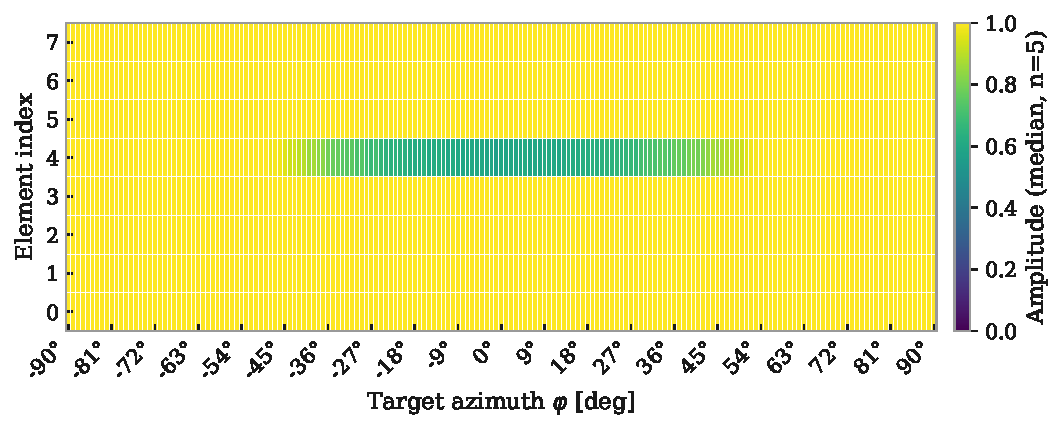
\includegraphics[width=\linewidth]{images/chapter5/ula8/amplitude_profile.pdf}
    \end{minipage}\hfill
    \begin{minipage}[t]{0.49\textwidth}
        \centering
        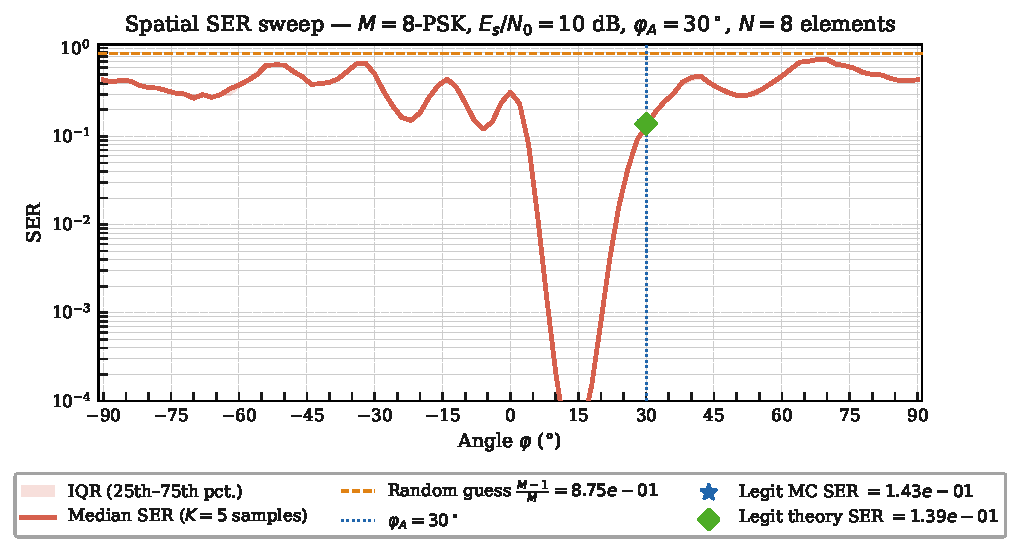
\includegraphics[width=\linewidth]{images/chapter5/ula8/ser_vs_angle.pdf}
    \end{minipage}\\[4pt]
    \begin{minipage}[t]{0.49\textwidth}
        \centering
        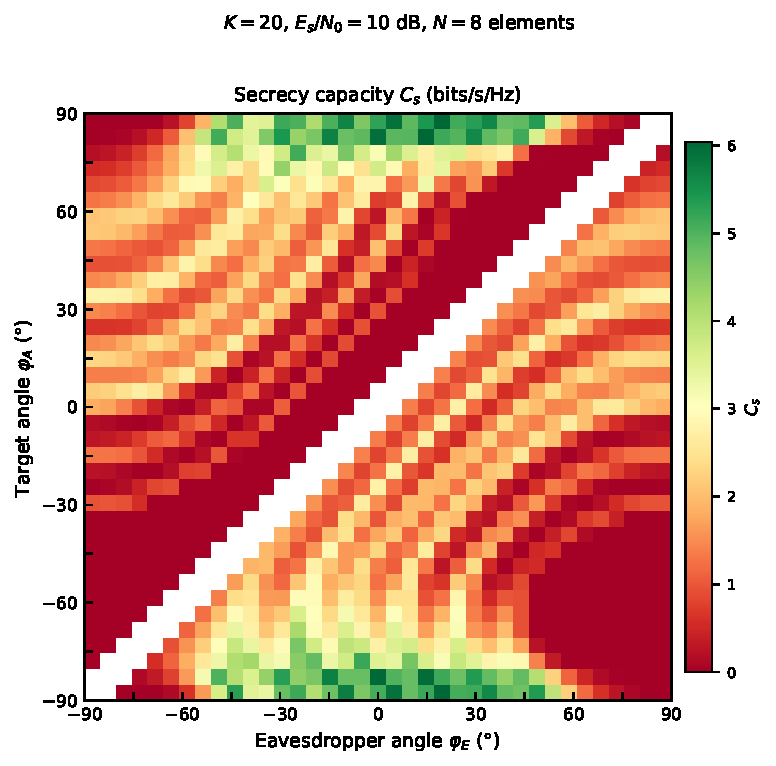
\includegraphics[width=\linewidth]{images/chapter5/ula8/secrecy_matrix.pdf}
    \end{minipage}\hfill
    \begin{minipage}[t]{0.49\textwidth}
        \centering
        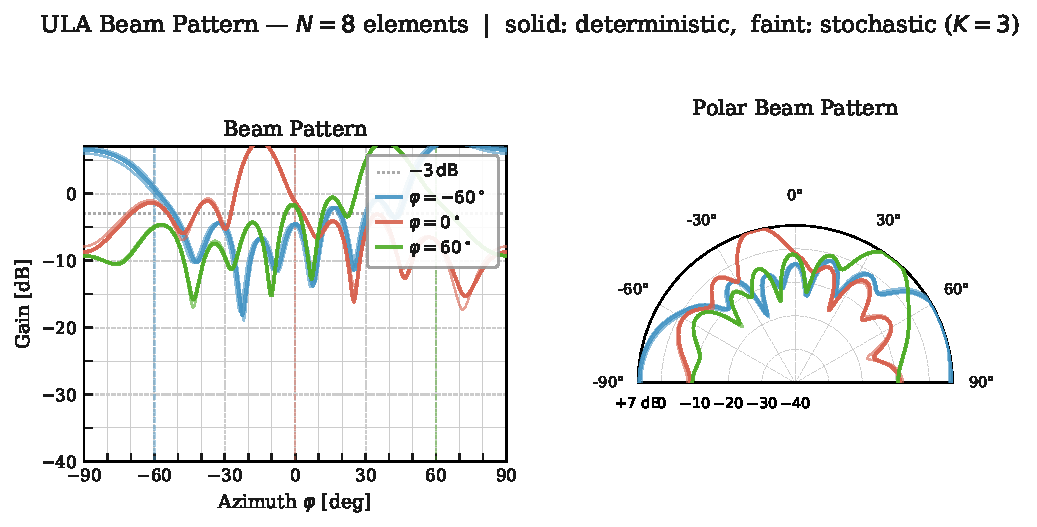
\includegraphics[width=\linewidth]{images/chapter5/ula8/beam_pattern.pdf}
    \end{minipage}
    \caption{Inference overview for the $N=8$\gls{ULA}. Top-left: amplitude profile across the full angular range.. Top-right:\gls{BER} vs.\ azimuth angle at $E_s/N_0 = 10$\,dB with the legitimate user at $\varphi = 30\degree$. Bottom-left: secrecy matrix. Bottom-right: beam patterns for $\varphi \in \{-60\degree, 0\degree, 60\degree\}$}
    \label{fig:ula8_inference}
\end{figure}

\begin{figure}[htbp]
    \centering
    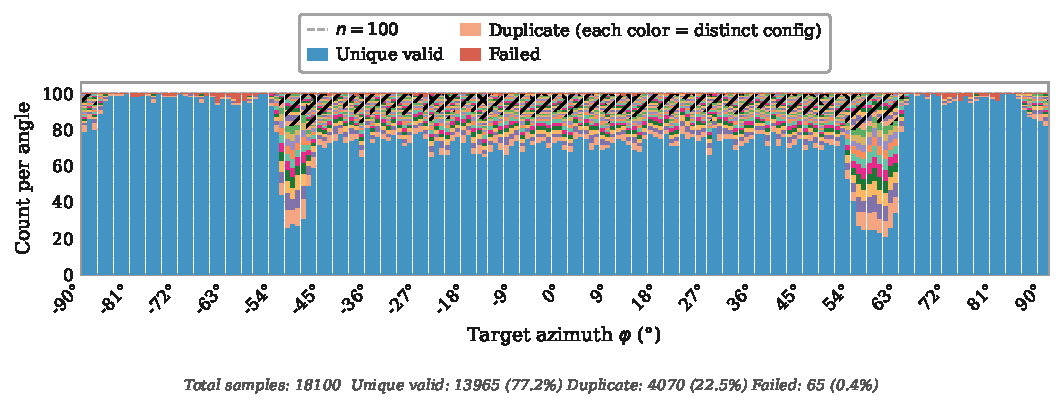
\includegraphics[width=1.0\textwidth]{images/chapter5/ula8/diversity_analysis.pdf}
    \caption{Outcome of 100 stochastic inference draws at each integer target angle $\varphi^* \in [-90\degree, 90\degree]$, for a total of 18{,}100 samples for the physics-informed action parameterisation with\gls{ULA} with $N=8$ elements. Each bar is decomposed into three categories: unique valid configurations (blue), duplicate solutions, and failed configurations that violated the amplitude or phase constraints (red).}
    \label{fig:ula8_diversity_analysis}
\end{figure}
\FloatBarrier             % Show the data gathered and analyze it
% !TEX encoding = UTF-8
% !TEX TS-program = pdflatex
% !TEX root = ../tesi.tex

%**************************************************************
\chapter{Conclusions}
\label{cap:conclusions}
%**************************************************************
{\color{blue} 

This thesis investigated the application of Reinforcement Learning (RL) to the problem of Dynamic Directional Modulation (DDM), with the objective of enabling the real-time generation of secure antenna array configurations that simultaneously satisfy communication and security constraints. Unlike conventional Directional Modulation approaches, which typically rely on deterministic optimization procedures to compute a single beamforming solution, Dynamic Directional Modulation requires the continuous generation of multiple valid configurations in order to prevent an eavesdropper from exploiting the static characteristics of the transmitted signal. This requirement naturally motivates a stochastic learning framework capable of producing a distribution of feasible solutions rather than a single deterministic optimum.

The first contribution of this work is the formulation of Dynamic Directional Modulation as a contextual bandit problem. Within this framework, the desired transmission direction acts as the context, while the antenna  phases constitute the action space. By learning a stochastic policy, the proposed approach is able to generate diverse antenna configurations that satisfy the desired radiation pattern constraints while maintaining the dynamic behaviour required by DDM. The results demonstrate that RL can effectively learn this mapping and perform inference in real time, replacing computationally expensive optimization procedures with a single forward pass through a neural network.

A second contribution is the geometric analysis of the DDM optimization problem. Through the study of the array factor and the phase-flatness constraint, it was shown that the difficulty of the problem is strongly dependent on the target direction. In particular, directions close to broadside were found to correspond to significantly smaller feasible regions in the solution space, making them intrinsically more challenging than directions near endfire. This observation provides an important physical interpretation of the learning dynamics and explains several convergence difficulties encountered during training.

Building upon this analysis, a third contribution of the thesis is the identification of a sampling imbalance introduced by conventional uniform-angle training strategies. Because the array response depends on the spatial-frequency variable $u=\sin(\varphi)$, uniform sampling in the angular domain does not correspond to a uniform coverage of the underlying physical problem. To address this issue, a sampling strategy based on uniform spacing in spatial-frequency space was proposed and integrated into the training process. This modification provides a more balanced representation of the problem domain and improves exploration of the most challenging regions of the angular range.

The fourth contribution is the development of a curriculum-learning framework specifically tailored to Dynamic Directional Modulation. The proposed curriculum progressively increases task complexity by initially focusing on the most difficult broadside directions and gradually expanding the angular range and tightening the design constraints. This strategy was found to significantly improve training stability and convergence, enabling the policy to discover feasible solutions in regions where direct training frequently struggled.

The experimental results illustrqte that the  learned policy is capable of producing distinct antenna excitation patterns for the same transmission direction while maintaining the desired radiation characteristics, thereby realizing the fundamental objective of Dynamic Directional Modulation. The approach performs particularly well for lower-order modulation schemes, while the results obtained for higher-order constellations reveal the increasing complexity of the underlying optimization landscape.

To sum-up, this thesis demonstrates that Reinforcement Learning provides a viable and flexible framework for Dynamic Directional Modulation. Beyond the successful application of RL itself, the work contributes new insights into the geometry of the DDM problem, highlights the importance of spatial-frequency-based sampling, and introduces curriculum-learning strategies that make the problem tractable in practice. These results establish a foundation for future research at the intersection of machine learning, antenna array processing, and physical-layer security.}

The proposed framework demonstrates promising results for lower modulation orders, successfully steering the array and maintaining acceptable symbol error rates under the simulated conditions. However, scalability remains a limiting factor: performance degrades notably at higher modulation orders such as 16-PSK, where the tighter noise margin amplifies the sensitivity to suboptimal beamforming configurations.
The central property of the framework is the stochasticity introduced at inference time: rather than a single deterministic output or a fixed beamforming configuration, the model generates a distribution of solutions, realising dynamic directional modulation.
The two training variations explored in this work reinforce this picture: the physics informed parameterisation confirms that embedding analytical structure in the action decoder is viable but reduces solution diversity and limits the policy's use of element-silencing strategies while the $N=8$ experiment shows that scaling the array exacerbates the model's limitations. Even the preferred gradient-based approach would require tuning, such as a larger exploration budget, a revised curriculum, or the use of known valid solutions as initialization points, to maintain the same quality of results achieved at $N=5$ when scaling with higher element numbers. 
The results are promising as a proof of concept, yet the gap between the simulated environment and real-world deployment remains substantial. Bridging this gap constitutes the primary direction for future development, as discussed in \chaptername~\ref{cap:future_works}.

%**************************************************************
\section{Future work}
\label{cap:future_works}
For future development on this thesis's groundwork, several directions to increase physical fidelity present themselves as natural extensions of this work.

\begin{itemize}
    \item \textbf{Hardware impairments and practical array constraints:} The current model assumes continuous-valued phase shifters and ideal, independent radiating elements; future works should incorporate finite phase-resolution constraints into the environment, alongside additional impairments such as nonlinear amplifiers, in-phase/quadrature imbalance, and oscillator noise. These effects introduce systematic deviations between the idealized steering vector and the physically realized beam pattern.
    \item \textbf{Multi-agent and distributed beamforming:} For very large arrays, such as those utilized in massive MIMO, centralized control of all antenna weights becomes computational prohibitive. A multi-agent reinforcement learning (MARL) formulation, in which individual agents govern sub-array or antenna panels and coordinate through limited inter-agent communication, offers a scalable alternative. 
    \item \textbf{Uniform Planar Array and full three-dimensional steering:} The current environment is restricted to a Uniform Linear Array (ULA) operating in the azimuth plane at a fixed elevation of $theta = 0^\circ$. Extending the geometry to a Uniform Planar Array (UPA) introduces a two-dimensional action space over both azimuth $\varphi$ and elevation $\theta$, increasing the dimensionality of the optimization problem and requiring the agent to learn a richer mapping from angular coordinates to beamforming weights.
    \item \textbf{Realistic channel models and multi-path propagation:} The reward signal currently evaluates beam quality against a free-space steering vector, which assumes a single line-of-sight propagation path. Practical wireless channels exhibit multi-path fading and Doppler shift. Replacing the idealized channel model with a standardized stochastic model would expose the agent to the full distribution of channel realizations it would encounter in real-world applications, promoting robustness over a wider range of propagation conditions. 
\end{itemize}

%**************************************************************
             % Conclusions
\appendix

\glsaddall[types={main}]
\printunsrtglossary[type=\acronymtype, style=nameparen]
\backmatter
\printbibliography
\end{document}
